\documentclass[Main.tex]{subfiles}
\begin{document}
	%%%Phần mở đầu
	\luuloigiai
	\setcounter{chapter}{4}
	\chapter{Năng lượng hóa học}
	\section{Phản ứng hóa học và entanpy}
	\begin{Muctieu}
		\begin{itemize}
			\item Phát biểu được khái niệm về phản ứng tỏa nhiệt, phản ứng thu nhiệt và biến thiên enthalpy của phản ứng.
			\item Trình bày được khái niệm về enthalpy tạo thành và tính được biến thiên enthalpy của phản ứng dựa vào enthalpy tạo thành.
			\item Nêu được ý nghĩa của dấu và giá trị của biến thiên enthalpy.
			\item Vận dụng được kiến thức về biến thiên enthalpy để giải thích một số hiện tượng thực tế.
		\end{itemize}
	\end{Muctieu}
	\begin{kd}
		Năng lượng hóa học là dạng năng lượng được lưu trữ trong các liên kết hóa học giữa các nguyên tử trong phân tử.Khi các liên kết hóa học bị phá vỡ hoặc hình thành trong quá trình phản ứng hóa học, năng lượng có thể được giải phóng (tỏa ra) hoặc hấp thụ (thu vào).\\
		\immini{Quan sát hình ảnh và cho biết phản ứng nào tỏa nhiệt, phản ứng nào thu nhiệt?}{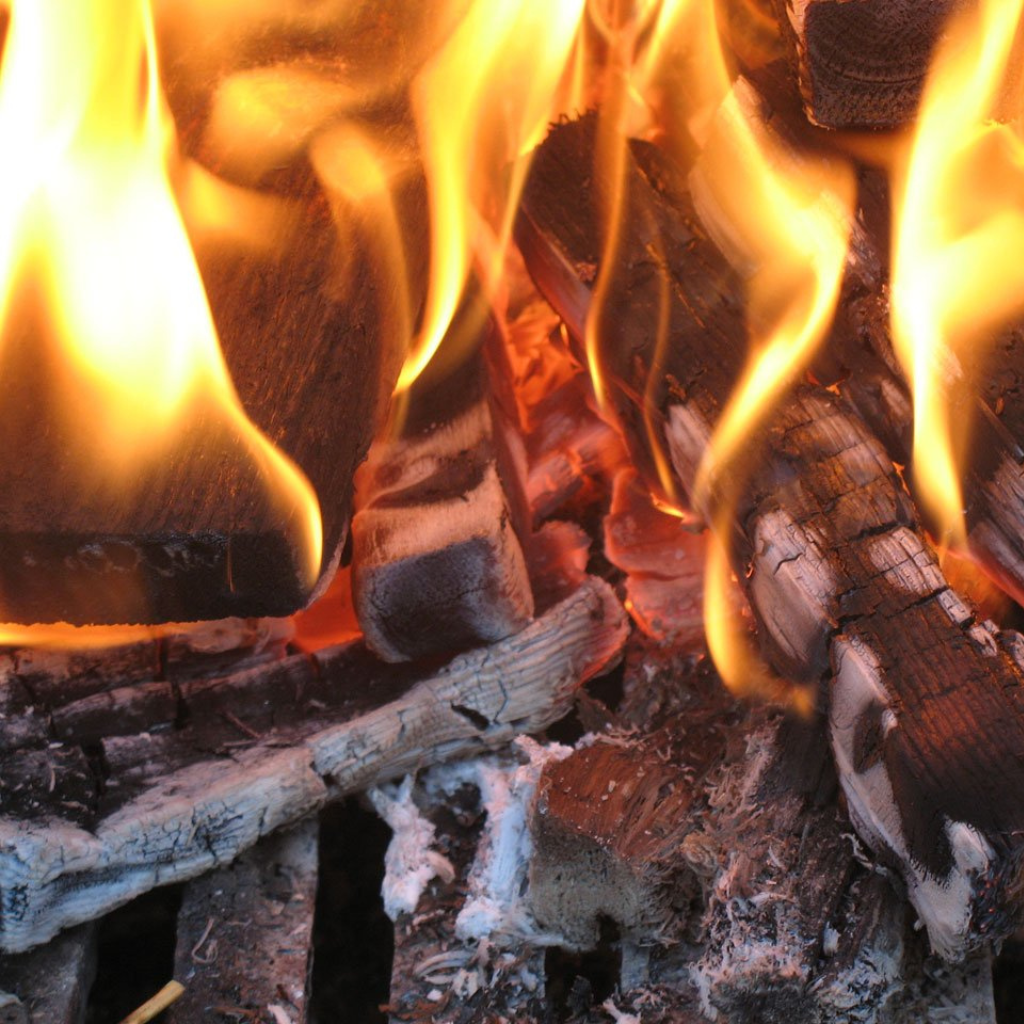
\includegraphics[width=5cm]{Images/anhhoahoc10/Nangluonghoahoc/phanungtoanhiet.png}\hspace{1cm}
\includegraphics[width=5cm]{Images/anhhoahoc10/Nangluonghoahoc/phanungthunhiet.png}}
	\end{kd}
	\subsection{Nội dung bài học}
	\subsubsection{Phản ứng tỏa nhiệt và phản ứng thu nhiệt}
	\Noibat[\maunhan][][][]{Phản ứng tỏa nhiệt}
	\begin{ghinho}
		\begin{enumerate}
			\item Phản ứng tỏa nhiệt là phản ứng giải phóng năng lượng dưới dạng nhiệt.
			\item Các phản ứng tỏa nhiệt có thể có hoặc không cần khơi mào, khi phản ứng đã xảy ra hầu hết không cần đun nóng tiếp.
			\item Ví dụ:
			\begin{itemize}
				\item  Đốt cháy khí metan ($CH_4$):
			$$
			\text{CH}_4 + 2\text{O}_2 \rightarrow \text{CO}_2 + 2\text{H}_2\text{O} + \text{nhiệt}
			$$
				\item  Phản ứng axit-bazơ:
			$$
			\text{HCl} + \text{NaOH} \rightarrow \text{NaCl} + \text{H}_2\text{O} + \text{nhiệt}
			$$
			\end{itemize}
		\end{enumerate}
	\end{ghinho}
	\Noibat[\maunhan][][][]{Phản ứng thu nhiệt}
	\begin{ghinho}
		\begin{enumerate}
			\item Phản ứng thu nhiệt là phản ứng hấp thu năng lượng dưới dạng nhiệt.
			\item Hầu hết các phản ứng thu nhiệt đều cần khơi mào và khi phản ứng xảy ra vẫn cần tiếp tục đun nóng.
			\item Ví dụ: Phản ứng nung đá vôi, hòa tan viên C sủi vào nước,$\ldots$ 
		\end{enumerate}
	\end{ghinho}
	\subsubsection{Biến thiên enthalpy của phản ứng và ý nghĩa}
		\begin{ghinho}
		   \Noibat[\maunhan][][\faStar][]{Một số từ viết tắt và kí hiệu}
			\begin{itemize}
				\item chất đầu (cd); sản phẩm (sp); phản ứng (reaction: r); tạo thành (fomation: f); chất rắn (solid: s); chất lỏng (liquid: l); chất khí (gas: g); chất tan trong nước (aqueous: aq) liên kết (bond: b).
			\end{itemize}
		\Noibat[\maunhan][][\faStar][]{Biến thiên enthalpy} (hay nhiệt phản ứng) là nhiệt lượng tỏa ra hoặc thu vào của phản ứng trong điều kiện áp suất không đổi.
			\begin{itemize}
				\item Kí hiệu: $\Delta_rH$; đơn vị: kJ hoặc kcal (1 J = $0{,}239$ cal)
			\end{itemize}
		\Noibat[\maunhan][][\faStar][]{Biến thiên enthalpy chuẩn}
		\begin{itemize}
			\item Điều kiện chuẩn (đkc): Nhiệt độ: 25$^\circ$C (hay 298K), áp suất 1 bar (đối với chất khí), nồng độ 1 mol/L (đối với chất tan trong dung dịch).
			\item Biến thiên enthalpy chuẩn ($\Delta_r H^\circ_{298}$) là nhiệt lượng tỏa ra hoặc thu vào của phản ứng ở điều kiện chuẩn.
			\item Phương trình nhiệt hóa học là phương trình hóa học kèm theo trạng thái các chất và nhiệt phản ứng. VD: $CH_{4(g)} + 2O_{2(g)} \rightarrow CO_{2(g)} + 2H_2O_{(l)} \quad \Delta_r H^\circ_{298} = -890.0 \text{ kJ}$
			\item Phương trình nhiệt hóa học cho biết: chất phản ứng, sản phẩm, tỉ lệ phản ứng, điều kiện phản ứng, trạng thái các chất và nhiệt phản ứng.
		\end{itemize}
		\end{ghinho}
	\subsubsection{Enthalpy tạo thành (nhiệt tạo thành)}
	\begin{ghinho}
		\begin{itemize}
			\item Enthalpy tạo thành hay nhiệt tạo thành ($\Delta_fH$) của một chất là biến thiên enthalpy của phản ứng tạo thành 1 mol chất đó từ các đơn chất ở trạng thái bền vững, ở một điều kiện xác định.\\[6pt]
			\textbf{\textit{Ví dụ:}} Ở điều kiện chuẩn, cần phải cung cấp $26{,}48$ kJ nhiệt lượng cho quá trình $0{,}5$ mol $H_2$(g) phản ứng với $0{,}5$ mol $I_2$(s) để thu được 1 mol HI(g).
			Như vậy enthalpy tạo thành của hydrogen iodide ở thể khí
			(HI) là $26{,}48$ kJ mol-1.
			\[
			\frac{1}{2}\mathrm{H}_{2}(g) + \frac{1}{2}\mathrm{I}_{2}(s) \rightarrow \mathrm{HI}(g) \quad \Delta_f H_{298}^{0} = 26,48 \, \mathrm{kJ} \, \mathrm{mol}^{-1}
			\]
			\item Nếu phản ứng thực hiện ở điều kiện chuẩn được gọi là enthalpy tạo thành chuẩn ($\Delta_fH^\circ_{298}$).
			\begin{itemize}
				\item $\Delta_fH^\circ_{298}$ của các đơn chất bền vững bằng 0.
				\item $\Delta_fH^\circ_{298} < 0 \Rightarrow$ chất bền hơn về mặt năng lượng so với các đơn chất tạo nên nó.
				\item $\Delta_fH^\circ_{298} > 0 \Rightarrow$ chất kém bền hơn về mặt năng lượng so với các đơn chất tạo nên nó.
			\end{itemize}
		\end{itemize}
	\end{ghinho}
	\begin{hopdongian}
		\textbf{Lưu ý:}
		\begin{itemize}
			\item Các giá trị $\Delta_fH^0_{298}$ thường được cho trong bảng tra cứu.
			\item Khi tính toán, cần chú ý đến hệ số tỉ lượng của các chất trong phương trình phản ứng.
		\end{itemize}
	\end{hopdongian}
	\subsubsection{Ý nghĩa của biến thiên enthalpy}
		\begin{ghinho}
			\begin{itemize}
				\item $\Delta_r H^\circ_{298} > 0$: Phản ứng thu nhiệt; $\Delta_r H^\circ_{298} < 0$: Phản ứng tỏa nhiệt.
				\item Giá trị tuyệt đối của $\Delta_r H^\circ_{298}$ càng lớn thì nhiệt lượng tỏa ra hoặc thu vào càng nhiều.
				\item Các phản ứng tỏa nhiệt thường diễn ra thuận lợi hơn phản ứng thu nhiệt.
			\end{itemize}
			\begin{center}
				\resizebox{!}{4cm}{\begin{tikzpicture}[declare function={r=3;}, line join=round, line cap=round, >=stealth, scale=1]
						\draw[\mycolor!80!black,>=stealth,->,text=\maunhan!80!black] (0,0) -- (0,5.25) node [pos=0.9, font=\scriptsize\bfseries\sffamily,anchor=east]{năng lượng};
						\draw[\mycolor!80!black,>=stealth,->,text=\maunhan!80!black] (0,0) -- (6.25,0) node [pos=1, font=\scriptsize\bfseries\sffamily,anchor=north east]{Tiến trình phản ứng} ;
						\draw[dashed,\mycolor!80!black,text=\maunhan!80!black] (0,1)node[left,font=\scriptsize\bfseries\sffamily]{$\Delta_{f}\text{H}^\circ_{298} \text{cđ}$}--(6,1);node
						\draw[dashed,\mycolor!80!black,text=\maunhan!80!black] (0,4)node[left,font=\scriptsize\bfseries\sffamily]{$\Delta_{f}\text{H}^\circ_{298} \text{sp}$}--(6,4)node [pos=0.5, font=\scriptsize\bfseries\sffamily,anchor=south,yshift=1cm]{phản ứng thu nhiệt};
						\draw[line width=1.2pt,\mycolor!80!black,text=\maunhan!80!black] 
						(0.5,1)--(3,1) node [pos=0.5, font=\scriptsize\bfseries\sffamily,anchor=north]{Chất phản ứng}--(3,4) node [pos=0.5, font=\scriptsize\bfseries\sffamily,anchor=west]{$\Delta_{r}\text{H}^\circ_{298} > 0$}
						(3,1) edge[-stealth] (3,4) 
						(3,4)--(6,4) node [pos=0.5, font=\scriptsize\bfseries\sffamily,anchor=south]{Sản phẩm};
				\end{tikzpicture}}
			\hspace{2cm}
			\resizebox{!}{4cm}{\begin{tikzpicture}[declare function={r=3;}, line join=round, line cap=round, >=stealth, scale=1]
					\draw[\mycolor!80!black,>=stealth,->,text=\maunhan!80!black] (0,0) -- (0,5.25) node [pos=0.9, font=\scriptsize\bfseries\sffamily,anchor=east]{năng lượng};
					\draw[\mycolor!80!black,>=stealth,->,text=\maunhan!80!black] (0,0) -- (6.25,0) node [pos=1, font=\scriptsize\bfseries\sffamily,anchor=north east]{Tiến trình phản ứng} ;
					\draw[dashed,\mycolor!80!black,text=\maunhan!80!black] (0,1)node[left,font=\scriptsize\bfseries\sffamily]{$\Delta_{f}\text{H}^\circ_{298} \text{sp}$}--(6,1);node
					\draw[dashed,\mycolor!80!black,text=\maunhan!80!black] (0,4)node[left,font=\scriptsize\bfseries\sffamily]{$\Delta_{f}\text{H}^\circ_{298} \text{cđ}$}--(6,4)node [pos=0.5, font=\scriptsize\bfseries\sffamily,anchor=south,yshift=1cm]{phản ứng tỏa nhiệt};
					\draw[line width=1.2pt,\mycolor!80!black,text=\maunhan!80!black] 
					(0.5,4)--(3,4)node [pos=0.5, font=\scriptsize\bfseries\sffamily,anchor=south]{Chất phản ứng}
					--(3,1)node [pos=0.5, font=\scriptsize\bfseries\sffamily,anchor=west]{$\Delta_{r}\text{H}^\circ_{298} < 0$}
					(3,4) edge[-stealth] (3,1)
					(3,1)--(6,1) node [pos=0.5, font=\scriptsize\bfseries\sffamily,anchor=north]{Sản phẩm};
			\end{tikzpicture}}
		
		  	\sffamily\textbf{Sơ đồ biểu diễn biến thiên enthalpy của phản ứng}
			\end{center}
		\end{ghinho}
	\subsection{Bài tập}
	
	
	%%%%%=====================Bài tập tự luận==========================%%%
	\phan{Bài tập tự luận}
	\Noibat[\maunhan][][\faBook][]{Bài tập minh họa}
	%%%=============SOẠN BT===============%%%
	\Opensolutionfile{ansbth}[Ans/LGBT-C05B01_Dang1]
	\Opensolutionfile{ansbt}[Ans/AnsBT-C05B01_Dang1]
	%%%==============BT_1==============%%%
	\begin{bt}
		Điền các từ hoặc cụm từ thích hợp vào chỗ trống:
		\begin{center}
			\begin{tabular}{|c|c|c|c|c|c|}
				\hline
				$25^\circ C$ (hay $298K$) & trạng thái & giải phóng & $1$ bar & nhiệt lượng & $1$ mol \\
				\hline
				nhiệt phản ứng & hấp thu & thu nhiệt & tỏa nhiệt & $1$ mol/L & bền vững \\
				\hline
			\end{tabular}
		\end{center}
		\begin{enumerate}
			\item[(a)] Phản ứng tỏa nhiệt là phản ứng \ldots (1) \ldots năng lượng dưới dạng nhiệt.
			
			Phản ứng thu nhiệt là phản ứng \ldots (2) \ldots năng lượng dưới dạng nhiệt.
			\item[(b)] Biến thiên enthalpy (hay nhiệt phản ứng) là \ldots (3) \ldots tỏa ra hoặc thu vào của phản ứng trong điều kiện áp suất không đổi.
			
			- Điều kiện chuẩn (đkc) ở nhiệt độ: \ldots (4) \ldots, áp suất \ldots (5) \ldots (đối với chất khí), nồng độ \ldots (6) \ldots (đối với chất tan trong dung dịch).
			
			- Phương trình nhiệt hóa học là phương trình hóa học kèm theo \ldots (7) \ldots các chất và \ldots (8) \ldots
			
			- $\Delta_r H_{298}^\circ > 0$: Phản ứng\ldots (9) \ldots; $\Delta_r H_{298}^\circ < 0$: Phản ứng\ldots (10) \ldots
			\item[(c)] Enthalpy tạo thành hay nhiệt tạo thành ($\Delta_f H$) của một chất là biến thiên enthalpy của phản ứng tạo thành \ldots (11) \ldots chất đó từ các đơn chất ở trạng thái \ldots (12) \ldots, ở một điều kiện xác định.
		\end{enumerate}
		\loigiai{
			(1) giải phóng; (2) hấp thu; (3) nhiệt lượng; (4) $25^\circ C$ (hay $298K$); (5) $1$ bar; (6) $1$ mol/L; (7) trạng thái; (8) nhiệt phản ứng; (9) thu nhiệt; (10) tỏa nhiệt; (11) $1$ mol; (12) bền vững.
		}
	\end{bt}
	\begin{bt}
		Phản ứng đốt cháy hoàn toàn 1 mol ethanol ($C_2H_5OH$) tỏa ra một lượng nhiệt là 1368 kJ. Viết phương trình nhiệt hóa học của phản ứng này.
		\loigiai{
			$C_2H_5OH(l) + 3O_2(g) \longrightarrow 2CO_2(g) + 3H_2O(l)  \quad \Delta_rH = -1368 \text{ kJ}$
		}
	\end{bt}
	%%%==============BT_2==============%%%
	\begin{bt}
		Đun nóng hai ống nghiệm: Ống (1) chứa bột potassium chlorate ($KClO_3$), ống (2) chứa bột sulfur (S), xảy ra các phản ứng:
		
		(1) $3KClO_3(s) \longrightarrow 2KCl(s) + 3O_2(g)$
		
		(2) $S(s) + O_2(g) \longrightarrow SO_2(g)$
		
		Khi ngừng đun, ở ống (1) phản ứng dừng lại, ở ống (2) phản ứng vẫn xảy ra. Hãy cho biết phản ứng nào là phản ứng tỏa nhiệt? phản ứng nào là phản ứng thu nhiệt?
		\loigiai{
			Phản ứng (1) là phản ứng thu nhiệt vì cần cung cấp nhiệt liên tục phản ứng mới xảy ra còn  phản ứng (2) là phản ứng tỏa nhiệt vì khi phản ứng đã xảy ra không cần cung cấp nhiệt.
		}
	\end{bt}
	%%%==============BT_3==============%%%
	\begin{bt}[][CD – SBT] Mỗi quá trình sau đây là thu nhiệt hay tỏa nhiệt?
		
		(1) $H_2O$ (lỏng, ở $25^\circ C$) $\longrightarrow$ $H_2O$ (hơi, ở $100^\circ C$).
		
		(2) $H_2O$ (lỏng, ở $25^\circ C$) $\longrightarrow$ $H_2O$ (rắn, ở $0^\circ C$).
		
		(3) $CaCO_3$ (Đá vôi) $\xrightarrow[Nung]$ $CaO + CO_2$.
		
		(4) Khí methane ($CH_4$) cháy trong oxygen.
		\loigiai{
			Các phản ứng chuyển trạng thái rắn $\longrightarrow$ lỏng $\longrightarrow$ khí (nhiệt độ tăng) là các phản ứng thu nhiệt vì cần phải cung cấp năng lượng để nâng nhiệt độ còn chuyển từ khí $\longrightarrow$ lỏng $\longrightarrow$ rắn là phản ứng tỏa nhiệt.
			
			$\Rightarrow$ (1) Thu nhiệt; (2) Tỏa nhiệt.
			
			(3) Thu nhiệt vì để phản ứng xảy ra cần phải đốt nóng liên tục.
			
			(4) Tỏa nhiệt vì phản ứng methane cháy làm không khí xung quanh nóng, tỏa nhiệt và phát sáng.
		}
	\end{bt}
	%%%==============BT_4==============%%%
	\begin{bt}
		Các quá trình sau thu nhiệt hay tỏa nhiệt? Giải thích ngắn gọn?
		\begin{enumerate}[(a)]
			\item Đốt một ngọn nến.
			\item Nước đóng băng.
			\item Hòa tan muối ăn vào nước thấy cốc nước trở nên mát.
			\item Luộc chín quả trứng.
			\item Hòa tan một ít bột giặt trong tay với nước, thấy tay ấm.
			\item Muối kết tinh từ nước biển ở các ruộng muối.
			\item Giọt nước đọng lại trên lá cây vào ban đêm.
			\item Đổ mồ hôi sau khi chạy bộ.
		\end{enumerate}
		\loigiai{
			\begin{enumerate}[(a)]
				\item Phản ứng tỏa nhiệt vì nến (parafin) bị đốt cháy đã giải phóng năng lượng, cung cấp cho việc phát sáng và tỏa nhiệt.
				\item Phản ứng tỏa nhiệt vì nước hạ nhiệt độ (hay giải phóng nhiệt) để tạo khối băng.
				\item Phản ứng thu nhiệt vì muối hấp thu nhiệt từ nước để hòa tan, nước giảm nhiệt độ và cốc nước trở nên mát.
				\item Phản ứng thu nhiệt vì trứng hấp thu nhiệt khiến các phân tử protein kết dính với nhau làm trứng chín.
				\item Phản ứng tỏa nhiệt. Vì khi hòa tan bột giặt trong tay với ít nước, bột giặt giải phóng nhiệt khi hòa tan, tạo phản ứng giúp loại bỏ nhanh các vết bẩn trên áo quần.
				\item Phản ứng thu nhiệt. Nước biển dưới ánh nắng mặt trời sẽ hấp thụ nhiệt và bay hơi, tạo thành nước biển kết tinh.
				\item[(h)] Phản ứng tỏa nhiệt. Ban đêm, hơi nước trong không khí hạ nhiệt để ngưng tụ, tạo thành các giọt đọng lại trên lá cây.
				\item Phản ứng thu nhiệt. Chạy bộ làm nhiệt độ cơ thể tăng. Khi đổ mồ hôi, một phần nước hấp thụ nhiệt và bay hơi. Sự bay hơi của mồ hôi giúp làm mát cơ thể và duy trì thân nhiệt ổn định.
			\end{enumerate}
		}
	\end{bt}
	%%%==============BT_5==============%%%
	\begin{bt}[][CD – SBT] Khi pha loãng $100$ ml $H_2SO_4$ đặc bằng nước thấy cốc đựng dung dịch nóng lên.
		
		Vậy quá trình pha loãng $H_2SO_4$ đặc là quá trình thu nhiệt hay tỏa nhiệt? Theo em, khi pha loãng $H_2SO_4$ đặc nên cho từ từ $H_2SO_4$ đặc vào nước hay ngược lại? Vì sao?
		\loigiai{
			Phản ứng tỏa nhiệt. Cần nhỏ từ từ $H_2SO_4$ đặc vào nước. Nếu làm ngược lại, do phản ứng tỏa nhiệt rất mạnh sẽ làm bắn $H_2SO_4$ ra xung quanh, gây mất an toàn và làm hư hại đồ vật, quần áo,...
		}
	\end{bt}
	
	%%%==============BT_6==============%%%
	\begin{bt}
		Cho các phương trình nhiệt hoá học:
		
		(1) $2Na HCO_3(s) $ $\xrightarrow[$t^\circ$]$ $ Na_2CO_3(s) + CO_2(g) + H_2O(g)\,\, \Delta_r H_{298}^\circ = +20{,}33\, kJ$
		
		(2) $4NH_3(g) + 3O_2(g)$ $\xrightarrow[$t^\circ$]$ $2N_2(g) + 6H_2O(l)\,\, \Delta_r H_{298}^\circ = -1531\, kJ$
		
		Các phương trình nhiệt hóa học trên cho biết những gì?
		\loigiai{
			Phản ứng (1) cho biết: Cứ $2$ mol $Na HCO_3$ ở thể rắn nhiệt phân tạo thành $1$ mol $Na_2CO_3$ ở thể rắn, $1$ mol $CO_2$ ở thể khí và $1$ mol $H_2O$ ở thể khí sẽ hấp thu nhiệt lượng là $20{,}33\, kJ$ $\Rightarrow$ Phản ứng thu nhiệt ($\Delta_r H_{298}^\circ > 0$)
			\\
			Phản ứng (2) cho biết: Khi đốt cháy $4$ mol $NH_3$ bằng $3$ mol $O_2$ tạo thành $2$ mol $N_2$, $6$ mol $H_2O$ sẽ tỏa ra nhiệt lượng là $1531\, kJ$ $\Rightarrow$ Phản ứng tỏa nhiệt ($\Delta_r H_{298}^\circ < 0$)
		}
	\end{bt}
	%%%==============BT_7==============%%%
	\begin{bt}
		Cho các phương trình nhiệt hoá học:
		
		(1) $CaCO_3(s) \longrightarrow CaO(s) + CO_2(g)\,\, \Delta_r H_{298}^\circ = +176{,}0\, kJ$
		
		(2) $C_2H_4(g) + H_2(g) \longrightarrow C_2H_6(g)\,\, \Delta_r H_{298}^\circ = -137{,}0\, kJ$
		
		(3) $Fe_2O_3(s) + 2Al(s) \longrightarrow Al_2O_3(s) + 2Fe(s)\,\, \Delta_r H_{298}^\circ = -851{,}5\, kJ$
		
		(4) $CO(g) + \dfrac{1}{2}O_2(g) \longrightarrow CO_2(g)\,\, \Delta_r H_{298}^\circ = -851{,}5\, kJ$
		
		(5) $C(graphite, s) + O_2(g) \longrightarrow CO_2(g)\,\, \Delta_r H_{298}^\circ = -393{,}5\, kJ$
		
		\begin{enumerate}
			\item[(a)] Trong các phản ứng trên, phản ứng nào tỏa nhiệt, phản ứng nào thu nhiệt?
			\item[(b)] Trong phương trình (2) và (5) thì enthalpy chuẩn của phản ứng có phải enthalpy tạo thành chuẩn của $C_2H_6$ và $CO_2$ không? Vì sao?
			\item[(c)] Vẽ sơ đồ biểu diễn biến thiên enthalpy của phản ứng (1) và (2).
		\end{enumerate}
		\loigiai{
			\begin{enumerate}
				\item[(a)] Phản ứng (1): thu nhiệt do $\Delta_r H_{298}^\circ > 0$
				
				Phản ứng (2), (3), (4), (5) : tỏa nhiệt do $\Delta_r H_{298}^\circ < 0$
				\item[(b)] Enthalpy chuẩn của phản ứng (2) không phải enthalpy tạo thành chuẩn của $C_2H_6$ do $C_2H_6$ trong phản ứng này không được tạo ra từ các đơn chất bền.
				
				Enthalpy chuẩn của phản ứng (5) là enthalpy tạo thành chuẩn của $CO_2$ do $CO_2$ trong phản ứng này được tạo ra từ các đơn chất bền.
				\item[(c)] {Sơ đồ biểu diễn biến thiên enthalpy của phản ứng (1), (2)}
				\begin{center}
					\begin{tikzpicture}[declare function={r=3;}, line join=round, line cap=round, >=stealth, scale=1]
						\draw[\mycolor!80!black,>=stealth,->,text=\maunhan!80!black] (0,0) -- (0,5.25) node [pos=0.9, font=\scriptsize\bfseries\sffamily,anchor=east]{Enthalpy, kJ};
						\draw[\mycolor!80!black,>=stealth,->,text=\maunhan!80!black] (0,0) -- (6.25,0) node [pos=1, font=\scriptsize\bfseries\sffamily,anchor=north east]{Tiến trình phản ứng} ;
						\draw[dashed,\mycolor!80!black,text=\maunhan!80!black] (0,1)node[left,font=\scriptsize\bfseries\sffamily]{$\Delta_{r}\text{H}^\circ_{298} \text{(cd)}$}--(3,1);
						\draw[dashed,\mycolor!80!black,text=\maunhan!80!black] (0,4)node[left,font=\scriptsize\bfseries\sffamily]{$\Delta_{r}\text{H}^\circ_{298} \text{(sp)}$}--(6,4);
						\draw[line width=1.2pt,\mycolor!80!black,text=\maunhan!80!black]
						(0.5,1)--(3,1) node [pos=0.5, font=\scriptsize\bfseries\sffamily,anchor=north]{$\text{CaCO}_3\text{(s)}$}--(3,4)
						(3,1) edge[-stealth] (3,4)
						(3,4)--(6,4) node [pos=0.5, font=\scriptsize\bfseries\sffamily,anchor=south]{$\text{CaO(s) + CO}_2\text{(g)}$};
						\node at (4.5,2.5) [font=\scriptsize\bfseries\sffamily] {$\Delta_{r}\text{H}^\circ_{298} = +176.0 \text{kJ}$};
					\end{tikzpicture}
					\hspace{0.5cm}
					\begin{tikzpicture}[declare function={r=3;}, line join=round, line cap=round, >=stealth, scale=1]
						\draw[\mycolor!80!black,>=stealth,->,text=\maunhan!80!black] (0,0) -- (0,5.25) node [pos=0.9, font=\scriptsize\bfseries\sffamily,anchor=east]{Enthalpy, kJ};
						\draw[\mycolor!80!black,>=stealth,->,text=\maunhan!80!black] (0,0) -- (6.25,0) node [pos=1, font=\scriptsize\bfseries\sffamily,anchor=north east]{Tiến trình phản ứng} ;
						\draw[dashed,\mycolor!80!black,text=\maunhan!80!black] (0,4)node[left,font=\scriptsize\bfseries\sffamily]{$\Delta_{r}\text{H}^\circ_{298} \text{(cd)}$}--(3,4);
						\draw[dashed,\mycolor!80!black,text=\maunhan!80!black] (0,1)node[left,font=\scriptsize\bfseries\sffamily]{$\Delta_{r}\text{H}^\circ_{298} \text{(sp)}$}--(6,1);
						\draw[line width=1.2pt,\mycolor!80!black,text=\maunhan!80!black]
						(0.5,4)--(3,4) node [pos=0.5, font=\scriptsize\bfseries\sffamily,anchor=south]{$\text{C}_2\text{H}_4\text{(g) + H}_2\text{(g)}$}
						--(3,1)
						(3,4) edge[-stealth] (3,1)
						(3,1)--(6,1) node [pos=0.5, font=\scriptsize\bfseries\sffamily,anchor=north]{$\text{C}_2\text{H}_6\text{(g)}$};
						\node at (4.5,2.5) [font=\scriptsize\bfseries\sffamily] {$\Delta_{r}\text{H}^\circ_{298} = -137.0 \text{kJ}$};
					\end{tikzpicture}
				\end{center}
			\end{enumerate}
		}
	\end{bt}
	%%%==============BT_8==============%%%
	\begin{bt}[][CTST - SBT] Cho các đơn chất sau đây: C(graphite, s); $Br_2(l)$; $Br_2(g)$; $Na(s)$; $Hg(l)$; $Hg(s)$.Đơn chất nào có $\Delta_f H_{298}^\circ = 0$?
		\loigiai{
			Các đơn chất C(graphite, s), $Br_2(l)$, $Na(s)$, $Hg(l)$, bền có $\Delta_f H_{298}^\circ = 0$.
		}
	\end{bt}
	%%%==============BT_9==============%%%
	\begin{bt}[][KNTT - SGK] Cho phản ứng:
		
		C(kim cương) $\longrightarrow$ C(graphite)\,\, $\Delta_r H_{298}^\circ = -1{,}9\, kJ$
		\begin{enumerate}
			\item[(a)] Ở điều kiện chuẩn, kim cương hay graphite có mức năng lượng thấp hơn?
			\item[(b)] Trong phản ứng xác định nhiệt tạo thành của $CO_2(g)$: $C(s) + O_2(g) \longrightarrow CO_2(g)$. Carbon ở dạng kim cương hay graphite?
		\end{enumerate}
		\loigiai{
			\begin{enumerate}
				\item[(a)] Mức năng lượng của graphite thấp hơn kim cương, graphite bền vững hơn.
				\item[(b)] Trong phản ứng xác định nhiệt tạo thành của $CO_2$, cacbon ở dạng graphite.
			\end{enumerate}
		}
	\end{bt}
	%%%==============BT_10==============%%%
	\begin{bt}
		[CD - SBT] Phân tử hemoglobin(Hb) trong máu nhận $O_2$ ở phổi để chuyển thành $HbO_2$. Chất này theo máu tới các bộ phận cơ thể, tại đó $HbO_2$ lại chuyển thành Hb và $O_2$( để cung cấp $O_2$ cho các hoạt động sinh hóa cần thiết trong cơ thể). Nếu trong không khí có lẫn carbon monoxide(CO), cơ thể nhanh chóng bị ngộ độc. Cho các số liệu thực nghiệm sau:
		
		$Hb + O_2 \longrightarrow HbO_2 \,\, \Delta_r H_{298}^\circ = -33{,}05kJ$  (1)
		
		$Hb + CO \longrightarrow HbCO \,\, \Delta_r H_{298}^\circ = -47{,}28kJ$ (2)
		
		$HbO_2 + CO \longrightarrow HbCO + O_2 \,\, \Delta_r H_{298}^\circ = -14{,}23kJ$ (3)
		
		$HbCO + O_2 \longrightarrow HbO_2 + CO \,\, \Delta_r H_{298}^\circ = 14{,}23\, kJ$ (4)
		
		Liên hệ giữa các mức độ thuận lợi các phản ứng (qua $\Delta_r H_{298}^\circ$) với những vấn đề thực nghiện nêu trên.
		\loigiai{
			Vì $\Delta_r H_{298}^\circ$ phản ứng (2) có âm hơn (1) và phản ứng (3) < (4) nên sự hình thành HbCO thuận lợi hơn sự tạo thành $HbO_2 \Rightarrow$ không có sự nhả $O_2$ và giải phóng Hb như trường hợp không có CO, điều này giải thích sự ngộ độc CO trong máu.
		}
	\end{bt}
%	\begin{bt}
%		Cho phản ứng: $N_2(g) + 3H_2(g) \longrightarrow 2NH_3(g)$. Biết enthalpy tạo thành chuẩn của $NH_3(g)$ là -46 kJ/mol. Tính biến thiên enthalpy chuẩn của phản ứng.
%		\loigiai{
%			\begin{eqnarray*}
%				\Delta_rH^0_{298} &=& 2\Delta_fH^0_{298}(\mathrm{NH}_3) - \left[\Delta_fH^0_{298}(\mathrm{N}_2) + 3\Delta_fH^0_{298}(\mathrm{H}_2)\right] \\
%				\Delta_rH^0_{298} &=& 2(-46) - \left[0 + 3(0)\right] = -92 \, \mathrm{kJ}/\mathrm{mol}
%			\end{eqnarray*}
%		}
%	\end{bt}
%	\begin{bt}
%		Tính biến thiên enthalpy của phản ứng sau: $2SO_2(g) + O_2(g) \longrightarrow 2SO_3(g)$ biết $\Delta_fH^0_{298}(SO_2) = -296.8$ kJ/mol và $\Delta_fH^0_{298}(SO_3) = -395.7$ kJ/mol
%		\loigiai{
%		\begin{eqnarray*}
%			\Delta_rH^0_{298} &=& 2\Delta_fH^0_{298}(\mathrm{SO}_3) - \left[2\Delta_fH^0_{298}(\mathrm{SO}_2) + \Delta_fH^0_{298}(\mathrm{O}_2)\right] \\
%			\Delta_rH^0_{298} &=& 2(-395.7) - \left[2(-296.8) + 0\right] = -197.8 \, \mathrm{kJ}/\mathrm{mol}
%		\end{eqnarray*}
%		}
%	\end{bt}
%	\begin{bt}
%		Tính lượng nhiệt tỏa ra khi đốt cháy hoàn toàn 16 gam khí methane ($CH_4$) biết $\Delta_fH^0_{298}(CH_4) = -74.6$ kJ/mol, $\Delta_fH^0_{298}(CO_2) = -393.5$ kJ/mol và $\Delta_fH^0_{298}(H_2O) = -285.8$ kJ/mol.
%		\loigiai{
%			Số mol $CH_4$ là $\frac{16}{16} = 1$ mol
%			\begin{eqnarray*}
%				\mathrm{CH}_4(g) + 2\mathrm{O}_2(g) &\longrightarrow& \mathrm{CO}_2(g) + 2\mathrm{H}_2\mathrm{O}(l) \\
%				\Delta_rH^0_{298} &=& \left[-393.5 + 2(-285.8)\right] - \left[-74.6 + 2(0)\right] \\
%				&=& -890.5 \, \mathrm{kJ}/\mathrm{mol}
%			\end{eqnarray*}
%			Vậy nhiệt tỏa ra khi đốt 16 gam $CH_4$ là 890.5 kJ
%		}
%	\end{bt}
%	\begin{bt}
%		Cho phản ứng: $2H_2(g) + O_2(g) \longrightarrow 2H_2O(l)$. Biết biến thiên enthalpy của phản ứng là -572 kJ. Tính enthalpy tạo thành chuẩn của $H_2O(l)$.
%		\loigiai{
%			\begin{eqnarray*}
%				\Delta_rH^0_{298} &=& 2\Delta_fH^0_{298}(\mathrm{H}_2\mathrm{O}) - \left[2\Delta_fH^0_{298}(\mathrm{H}_2) + \Delta_fH^0_{298}(\mathrm{O}_2)\right] \\
%				-572 &=& 2\Delta_fH^0_{298}(\mathrm{H}_2\mathrm{O}) - \left[0 + 0\right] \\
%				\Delta_fH^0_{298}(\mathrm{H}_2\mathrm{O}) &=& -286 \, \mathrm{kJ}/\mathrm{mol}
%			\end{eqnarray*}
%		}
%	\end{bt}

	\Closesolutionfile{ansbt}
	\Closesolutionfile{ansbth}
	%\bangdapanSA{AnsBT-C05B01_Dang1}
	\newpage
	\begin{hopdongian}
		\Noibat[\maunhan][\large\bfseries\fontfamily{qag}\selectfont][\faApple][]{Bài toán tính theo phương trình nhiệt hóa học}
		\begin{itemize}
			\item Phương trình nhiệt hóa học là phương trình hóa học kèm theo trạng thái các chất và nhiệt phản ứng.
			\item Biến thiên enthalpy trong phương trình nhiệt hóa học tỉ lệ với hệ số các chất trong phương trình.
			\item Có thể xử lý các phương trình nhiệt hóa như những phương trình đại số (cộng, trừ, nhân với một hệ số, đổi chiều \ldots thì $\Delta_r H^\circ_{298}$ cũng chịu cùng cách xử lý).
		\end{itemize}
	\end{hopdongian}
	\Noibat[\maunhan][][\faBookmark][]{Ví dụ mẫu}

	%%%=============SOẠN BT===============%%%
	\Opensolutionfile{ansbth}[Ans/LGBT-C05B01_VDM_DANG1]
	\Opensolutionfile{ansbt}[Ans/AnsBT-C05B01_VDM_DANG1]
		%%%==============BT_11==============%%%
	\begin{bt}[][KNTT - SGK] Biết phản ứng đốt cháy khí carbon monoxide (CO) như sau:
		
		$CO(g) + \dfrac{1}{2}O_2(g) \longrightarrow CO_2(g)\,\, \Delta_r H_{298}^\circ = -851{,}5\, kJ$
		
		\begin{enumerate}
			\item[(a)] Ở điều kiện chuẩn, nếu đốt cháy hoàn toàn $2{,}479$ L khí CO thì nhiệt lượng tỏa ra là bao nhiêu?
			\item[(b)] Ở điều kiện chuẩn, nếu nhiệt lượng tỏa ra $1277{,}25\, kJ$ thì thể tích khí CO đã dùng là bao nhiêu L?
		\end{enumerate}
		\loigiai{
			Theo phương trình nhiệt hóa học ta có: Cứ đốt cháy $1$ mol CO thì nhiệt lượng tỏa ra là $851{,}15\, kJ$.
			
			(a) Ta có: $n_{CO} = \dfrac{2{,}479}{24{,}79} = 0{,}1\, mol \Rightarrow$ Nhiệt lượng tỏa ra là: $0{,}1.851{,}5 = 85{,}15\, kJ$
			
			(b) Ta có: $n_{CO} = \dfrac{1277{,}25}{851{,}5} = 1{,}5\, mol \Rightarrow$ Thể tích CO đã dùng ở đkc là $V_{CO} = 1{,}5.24{,}79 = 37{,}185(L)$.
		}
	\end{bt}
	%%%==============BT_12==============%%%
	\begin{bt}
		[CD - SGK] Cho phản ứng: $N_2(g) + 3H_2(g) \longrightarrow 2NH_3(g)$
		
		Ở điều kiện chuẩn, cứ $1$ mol $N_2$ phản ứng hết sẽ tỏa ra $92{,}22$ kJ. Tính enthalpy tạo thành chuẩn của $NH_3$.
		\loigiai{
			Từ phản ứng ta thấy
			
			Cứ $1$ mol $N_2$ phản ứng hết tạo ra $2$ mol $NH_3$ và tỏa ra $99{,}22$ kJ
			
			Cần $0{,}5$ mol $N_2$ phản ứng hết tạo ra $1$ mol $NH_3$ và tỏa ra x kJ
			
			$\Rightarrow x = \dfrac{99{,}22}{2} = 49{,}61kJ$
			
			$\Rightarrow \Delta_f H_{298}^\circ = -49{,}61kJ\, mol^{-1}$ (enthalpy có giá trị âm vì đây là phản ứng tỏa nhiệt)
		}
	\end{bt}
	%%%==============BT_13==============%%%
	\begin{bt}[][KNTT - SBT] Tính biến thiên enthalpy chuẩn theo các phương trình phản ứng sau, biết nhiệt tạo thành chuẩn của $NH_3$ bằng $-46$ kJ/mol.
		
		$N_2(g) + 3H_2(g) \longrightarrow 2NH_3(g)$ (1)
		
		$\dfrac{1}{2}N_2(g) + \dfrac{3}{2}H_2(g) \longrightarrow NH_3(g)$ (2)
		
		\begin{enumerate}
			\item[(a)] Tính $\Delta_r H_{298}^\circ$ (1) và $\Delta_r H_{298}^\circ$ (2), so sánh $\Delta_r H_{298}^\circ$ (1) và $\Delta_r H_{298}^\circ$ (2)
			\item[(b)] Khi tổng hợp được $1$ tấn $NH_3$ thì nhiệt lượng tỏa ra hay thu vào là bao nhiêu? (Tính theo cả $2$ phương trình trên và đưa ra nhận xét)
		\end{enumerate}
		\loigiai{
			\begin{enumerate}
				\item[(a)] $\Delta_r H_{298}^\circ(1) = 2.(-46) - 1.0 - 3.0 = -92\, kJ$
				
				$\Delta_r H_{298}^\circ(2) = (-46) - \dfrac{1}{2}.0 - \dfrac{3}{2}.0 = -46\, kJ$
				
				Phản ứng tỏa nhiệt và $\Delta_r H_{298}^\circ(1) = 2. \Delta_r H_{298}^\circ(2)$
				\item[(b)] Khi tổng hợp $1$ tấn $NH_3$ thì nhiệt lượng tỏa ra $= \dfrac{46.10^6}{17} = 2{,}7.10^6 (kJ)$
				
				Tính theo $2$ phương trình trên thì đều ra kết quả giống nhau.
			\end{enumerate}
		}
	\end{bt}
	%%%==============BT_14==============%%%
	\begin{bt}[][CTST - SBT] Cho phản ứng:
		
		$2ZnS(s) + 3O_2(g) \longrightarrow 2ZnO(s) + 2SO_2(g)\,\, \Delta_r H_{298}^\circ = -285{,}66\, kJ$
		
		Xác định giá trị của $\Delta_r H_{298}^\circ$ khi:
		\begin{enumerate}
			\item[(a)] Lấy gấp $3$ lần khối lượng của các chất phản ứng.
			\item[(b)] Lấy một nửa khối lượng của các chất phản ứng.
			\item[(c)] Đảo chiều của phản ứng.
		\end{enumerate}
		\loigiai{
			\begin{enumerate}
				\item[(a)] Nhân phương trình của phản ứng với 3: $\Delta_r H_{298}^\circ = -285{,}66 x 3 = -856{,}98\, kJ$
				\item[(b)] Chia phương trình của phản ứng với 2: $\Delta_r H_{298}^\circ = -285{,}66 : 2 = -142{,}83\, kJ$
				\item[(c)] Đảo chiều của phản ứng: $\Delta_r H_{298}^\circ = +285{,}66\, kJ$
			\end{enumerate}
		}
	\end{bt}
	%%%==============BT_15==============%%%
	\begin{bt}[][CTST - SBT] Viết phương trình nhiệt hóa học của các quá trình tạo thành những chất dưới đây từ đơn chất ở điều kiện chuẩn:
		\begin{enumerate}
			\item[(a)] Nước ở trạng thái, biết rằng khi tạo thành $1$ mol hơi nước tỏa ra $214{,}6$ kJ nhiệt.
			\item[(b)] Nước lỏng, biết rằng sự tạo thành $1$ mol nước lỏng tỏa ra $285{,}49$ kJ nhiệt.
			\item[(c)] Ammonia ($NH_3$), biết rằng sự tạo thành $2{,}5$ g ammonia tỏa ra $22{,}99$ kJ nhiệt.
			\item[(d)] Phản ứng nhiệt phân đá vôi ($CaCO_3$), biết rằng để thu được $11{,}2$ g vôi (CaO) phải cung cấp $6{,}94$ kcal.
		\end{enumerate}
		\loigiai{
			\begin{enumerate}
				\item[(a)] $H_2(g) + \dfrac{1}{2}O_2(g) \longrightarrow H_2O(g)\,\, \Delta_r H_{298}^\circ = -214{,}6\, kJ$
				\item[(b)] $H_2(g) + \dfrac{1}{2}O_2(g) \longrightarrow H_2O(l)\,\, \Delta_r H_{298}^\circ = -285{,}49\, kJ$
				\item[(c)] Số mol ammonia $= \dfrac{5}{34}$ mol. $1$ mol ammonia tỏa ra $22{,}99 : \dfrac{5}{34} = 156{,}332$ kJ nhiệt.
				
				$\dfrac{3}{2}H_2(g) + \dfrac{1}{2}N_2(g) \longrightarrow NH_3(g)\,\, \Delta_r H_{298}^\circ = -156{,}332\, kJ$
				\item[(d)] $n_{CaO} = 0{,}2$ mol $\Rightarrow$ Để tạo thành $1$ mol CaO cần cung cấp $6{,}94.5 = 34{,}7$ kcal.
				
				$CaCO_3(s) \xrightarrow{t^\circ} CO_2(g) + CaO(s)\,\, \Delta_r H_{298}^\circ = +34{,}7$ kcal
			\end{enumerate}
		}
	\end{bt}
	%%%==============BT_16==============%%%
	\begin{bt}[][CTST - SBT] Lactic acid hay acid sữa là hợp chất hóa học đóng vai trò quan trọng trong nhiều quá trình sinh hoá, lần đầu tiên được phân tách vào năm $1780$ bởi nhà hóa học Thụy Điển Carl Wilhelm Scheele. Lactic acid có công thức phân tử $C_3H_6O_3$, công A thức cấu tạo $CH_3-CH(OH)-COOH$.
		
		Khi vận động mạnh cơ thể không đủ cung cấp oxygen, thì cơ thể sẽ chuyển hoá glucose thành lactic acid từ các tế bào để cung cấp năng lượng cho cơ thể (lactic acid tạo thành từ quá trình này sẽ gây mỏi cơ) theo phương trình sau:
		
		$C_6H_{12}O_6(aq) \longrightarrow 2C_3H_6O_3(aq)\,\, \Delta_r H_{298}^\circ = -150\, kJ$
		
		Biết rằng cơ thể chỉ cung cấp $98\%$ năng lượng nhờ oxygen, năng lượng còn lại nhờ vào sự chuyển hoá glucose thành lactic acid.
		
		Giả sử một người chạy bộ trong một thời gian tiêu tốn $300$ kcal. Tính khối lượng lactic acid tạo ra từ quá trình chuyển hoá đó (biết $1$ cal $= 4{,}184$ J).
		\loigiai{
			Tính khối lượng lactic acid tạo ra từ quá trình chạy bộ. Năng lượng của sự chuyển hoá glucose thành lactic acid trong quá trình chạy bộ chiếm $2\% x 300$ kcal $= 6$ kcal $= 6 000$ cal $\Leftrightarrow 25 104 J = 25{,}104\, kJ$.
			
			\begin{tabular}{ccc}
				$C_6H_{12}O_6$ & $\longrightarrow 2C_3H_6O_3$ & $\Delta_r H_{298}^\circ = -150\, \text{kJ}$ \\
				$0{,}335$ mol & & $-25{,}104$ kJ
			\end{tabular}
			
			Khối lượng lactic acid được tạo ra trong quá trình chuyển hóa: $0{,}335 x 90 = 30{,}15$ g.
		}
	\end{bt}
	%%%==============BT_17==============%%%
	\begin{bt}
		Cho các phương trình nhiệt hóa học sau:
		
		(1) $C(graphite) + O_2(g) \longrightarrow CO_2(g)\,\, \Delta_r H_{298}^\circ (1) = -393{,}5\, kJ$
		
		(2) $C(graphite) \longrightarrow C(kim\, cuong)\,\, \Delta_r H_{298}^\circ (2) = 2{,}87\, kJ$
		
		(3) $C(kim\, cuong) + O_2(g) \longrightarrow CO_2(g)\,\, \Delta_r H_{298}^\circ (3) = ?\, kJ$
		
		Hãy tính $\Delta_r H_{298}^\circ$ của phản ứng (3)?
		\loigiai{
			Ta có: (1) – (2) = (3) $\Rightarrow \Delta_r H_{298}^\circ (3) = \Delta_r H_{298}^\circ (1) - \Delta_r H_{298}^\circ (2) = -393{,}5 - 2{,}87 = -396{,}37\, kJ$
		}
	\end{bt}
	
	%%%==============BT_18==============%%%
	\begin{bt}
		Cho các phương trình nhiệt hóa học sau:
		
		(1) $Mg(s) + 2HCl(aq) \longrightarrow MgCl_2(aq) + H_2(g)\,\, \Delta_r H_{298}^\circ (1) = -467{,}0\, kJ$
		
		(2) $MgO(s) + 2HCl(aq) \longrightarrow MgCl_2(aq) + H_2O(l)\,\, \Delta_r H_{298}^\circ (2) = -151{,}0\, kJ$
		
		và $\Delta_f H_{298}^\circ (H_2O, l) = -286\, kJ/mol$. Tính enthalpy tạo thành chuẩn của MgO(s)
		\loigiai{
			Ta có: (3) $H_2(g) + \dfrac{1}{2}O_2(g) \longrightarrow H_2O(l)\,\, \Delta_r H_{298}^\circ (3) = -286kJ$
			
			(4) $Mg(s) + \dfrac{1}{2}O_2(g) \longrightarrow MgO(s)\,\, \Delta_r H_{298}^\circ (4) = ?\, kJ$.
			
			Ta có: (4) = (1) – (2) + (3) $\Rightarrow \Delta_r H_{298}^\circ (4) = -467 - (-151) + (-286) = -602\, kJ$
			
			$\Rightarrow$ Enthalpy tạo thành chuẩn của MgO(s) là $\Delta_f H_{298}^\circ$ (MgO, s) $= -602$ kJ/mol
		}
	\end{bt}
	%%%==============BT_19==============%%%
	\begin{bt}[][CD - SBT] Biến thiên enthalpy chuẩn quá trình "$H_2O(s) \longrightarrow H_2O(l)$" là $6{,}020kJ$.
		\begin{enumerate}
			\item[(a)] Quá trình tan chảy của nước đá là quá trình thu nhiệt hay tỏa nhiệt? Vì sao?
			\item[(b)] Vì sao khi cho viên nước đá vào cốc nước lỏng ấm, viên đá lại tan chảy dần?
			\item[(c)] Vì sao cốc nước lỏng bị lạnh dần trong quá trình viên nước đá tan chảy?
			\item[(d)] Biết rằng để làm cho nhiệt độ của $1$ mol nước lỏng thay đổi $1^\circ C$ cần một nhiệt lượng là $75{,}4J$. Giả sử mỗi viên nước đá tương ứng với $1$ mol nước, hãy xác định số viên nước đá tối thiểu cần tan chảy để có thể làm lạnh $500$ gam nước lỏng ở $20^\circ C$ xuống $0^\circ C$.
			\item[(e)] Để làm lạnh $120$ gam nước lỏng ở $45^\circ C$ xuống $0^\circ C$, một bạn học sinh đã dùng $150$ gam nước đá. Lượng nước đá này là vừa đủ, thiếu hay dư? (Trong phần d, e giả thiết có sự trao đổi nhiệt giữa nước và nước đá)
		\end{enumerate}
		\loigiai{
			\begin{enumerate}
				\item[(a)] Quá trình tan chảy của nước đá là quá trình thu nhiệt vì có biến thiên enthalpy dương.
				\item[(b)] Viên đá lại tan chảy dần vì nó lấy nhiệt từ nước lỏng( là môi trường xung quanh)
				\item[(c)] Nước lỏng nhường nhiệt cho viên nước đá, sự mất nhiệt làm cho nước lỏng lạnh đi.
				\item[(d)] Nhiệt lượng mà $500$ gam nước lỏng từ ở $20^\circ C$ xuống $0^\circ C$ tỏa ra là:
				
				$\dfrac{500}{18}.75{,}4.(20-0) = 41888{,}9 (J) = 41{,}8889 (kJ)$
				
				Mỗi viên đá tan chảy hấp thụ một nhiệt lượng là $6{,}020$ kJ
				
				$\Rightarrow$ Số viên nước đá tối thiểu cần là $\dfrac{41{,}8889}{6{,}02} = 6{,}96 \approx 7$ viên.
				\item[(e)] Nhiệt lượng mà $120gam$ nước lỏng ở $45^\circ C$ xuống $0^\circ C$ tỏa ra là:
				
				$\dfrac{120}{18}.75{,}4.(45-0) = 22620 (J) \Rightarrow$ Lượng nước đá cần dùng là: $(22620 : 6020) x 18 = 67{,}63 (g)$
				
				Vậy dùng $150$ gam nước đá là dư
			\end{enumerate}
		}
	\end{bt}
	%%%==============BT_20==============%%%
	\begin{bt}[][CD – SBT] Nhiệt tỏa ra khi đốt cháy $1$ gam một mẫu than là $23{,}0$ kJ. Giả thiết rằng toàn bộ lượng nhiệt của quá trình đốt than tỏa ra đều dùng để làm nóng nước, không có sự thất thoát nhiệt, hãy tính lượng than cần phải đốt để làm nóng $500$ gam nước từ $20^\circ C$ tới $90^\circ C$. Biết để làm nóng $1$ mol nước thêm $1^\circ C$ cần một nhiệt lượng là $75{,}4$ J.
		\loigiai{
			Lượng nhiệt cần dùng để đun nóng $500$ gam nước từ $20^\circ C$ lên $90^\circ C$ là
			
			$\dfrac{500}{18}.75{,}4.(363-293) = 146611{,}1(J)$
			
			Vậy lượng than đá cần dùng là: $\dfrac{146611{,}1}{23.10^3} = 6{,}37 (g)$.
		}
	\end{bt}
	%%%=============BT_21=============%%%
	\begin{bt}
		Ở một lò nung vôi công nghiệp, cứ sản xuất được $1000$ kg vôi sống cần dùng m kg than đá (chứa $80\%$ carbon) làm nhiên liệu cung cấp nhiệt.
		\\
		Cho các phản ứng: $C(s)+O_2(g) \longrightarrow CO_2(g) \quad \Delta_r H_{298}^0 = -393{,}5$ kJ/mol
		\\
		$CaCO_3(s) \longrightarrow CaO(s)+CO_2(s) \quad \Delta_r H_{298}^0 =178{,}29$kJ
		\\
		Biết hiệu suất hấp thụ ở quá trình phân hủy đá vôi là $60\%$. Tính giá trị của m.
		\loigiai{
			Để thu được $1000$ kg $CaO$ thì nhiệt lượng cần cung cấp (với hiệu suất là $60\%$)
			\\
			$\dfrac{1000.10^3}{56}.\dfrac{178{,}29}{0{,}6} = 5306{,}25.10^3$ kJ
			\\
			Ta có: $5306{,}25.10^3 = \dfrac{m.10^3.0{,}8}{12}.393{,}5 \Rightarrow m = 202{,}27$ kg.
		}
	\end{bt}
	%%%=============BT_22=============%%%
	\begin{bt}
		Một mẫu khí gas X chứa hỗn hợp propane và butane.
		\\
		Cho các phản ứng: $C_3H_8(g) + 5O_2(g) \longrightarrow 3CO_2(g) + 4H_2O(l) \quad \Delta_r H_{298}^0 = -2220$kJ
		\\
		$C_4H_{10}(g) + \dfrac{13}{2}O_2(g) \longrightarrow 4CO_2(g) + 5H_2O(l) \quad \Delta_r H_{298}^0 = -2874$kJ
		\\
		Đốt cháy hoàn toàn $12$ gam mẫu khí gas X tỏa ra nhiệt lượng $597{,}6$ kJ. Xác định tỉ lệ số mol của propane và butane trong X.
		\loigiai{
			Gọi
			$\begin{cases}
				n_{C_3H_8} = a \, (mol) \\
				n_{C_4H_{10}} = b \, (mol)
			\end{cases} \longrightarrow 44a + 58b = 12 \,\, (1)$
			\\
			$12$ gam X tỏa ra lượng nhiệt là: $2220.a + 2874.b = 597{,}6$ kJ $(2)$
			\\
			Từ $(1)$ và $(2)$ ta có hệ phương trình:
			$\begin{cases}
				44a + 58b = 12 \\
				2220a + 2874b = 597{,}6
			\end{cases} \longrightarrow \begin{cases}
				a = 0{,}075 \\
				b = 0{,}15
			\end{cases}$
			\\
			$\rightarrow$ a : b = 1 : 2.
		}
	\end{bt}
	\Closesolutionfile{ansbt}
	\Closesolutionfile{ansbth}
	%\bangdapanSA{AnsBT-C05B01_VDM_DANG1}
	\Noibat[\maunhan][][\faStar][]{Bài tập tự luyện}
	%%%=============SOẠN BT===============%%%
	\Opensolutionfile{ansbth}[Ans/LGBT-C05B01_BTTL_DANG1]
	\Opensolutionfile{ansbt}[Ans/AnsBT-C05B01_BTTL_DANG1]
		\begin{bt}[][CTST - SGK] Phân biệt enthalpy tạo thành của một chất và biến thiên enthalpy của phản ứng. Lấy ví dụ minh họa.
		\loigiai{
			- Enthalpy tạo thành của một chất là nhiệt kèm theo phản ứng tạo thành $1$ mol chất đó từ các đơn chất bền nhất.
			\\
			- Biến thiên Enthalpy của phản ứng là nhiệt lượng tỏa ra hay thu vào của một phản ứng hóa học trong quá trình đẳng áp (áp suất không đổi)
			
			\begin{tabular}{|l|l|}
				\hline
				\textbf{Enthalpy tạo thành của một chất} & \textbf{Biến thiên enthalpy của phản ứng} \\
				\hline
				- Chất tham gia phải là đơn chất bền nhất. & - Chất tham gia ở dạng đơn chất hay hợp chất đều được. \\
				\hline
				- Sản phẩm chỉ có $1$ chất duy nhất. & - Sản phẩm có thể là $1$ hay nhiều chất. \\
				\hline
				- VD: & - VD: \\
				$C$(graphite, s) + $O_2(g) \longrightarrow CO_2(g)$ & $C_2H_4(g) + H_2(g) \longrightarrow C_2H_6(g)$ \\
				$\Delta_r H_{298}^0 = -393{,}5$ kJ / mol & $\Delta_r H_{298}^0 = -137{,}0$ kJ \\
				\hline
			\end{tabular}
		}
	\end{bt}
	%%%=============BT_24=============%%%
	\begin{bt}[][CD - SGK] Dự đoán các phản ứng sau đây là tỏa nhiệt hay thu nhiệt?
		\begin{enumerate}
			\item Nung $NH_4Cl(s)$ tạo ra $HCl(g)$ và $NH_3(g)$.
			\item Cồn cháy trong không khí.
			\item Phản ứng thủy phân collagen thành gelain (là một loại protein dễ tiêu hóa) diễn ra khi hầm xương động vật.
		\end{enumerate}
		\loigiai{
			\begin{enumerate}
				\item Nung $NH_4Cl(s)$ tạo ra $HCl(g)$ và $NH_3(g)$ là phản ứng thu nhiệt.
				\\
				Giải thích: Do cần cung cấp nhiệt trong suốt quá trình phản ứng.
				\item Cồn cháy trong không khí là phản ứng tỏa nhiệt.
				\\
				Giải thích: Do phản ứng đốt cháy cồn chỉ cần cung cấp nhiệt vào thời điểm ban đầu và có tỏa nhiệt trong quá trình phản ứng
				\item Phản ứng thủy phân collagen thành gelain (là một loại protein dễ tiêu hóa) diễn ra khi hầm xương động vật là phản ứng thu nhiệt.
				\\
				Giải thích: Do cần cung cấp nhiệt trong suốt quá trình phản ứng (hầm).
			\end{enumerate}
		}
	\end{bt}
	%%%=============BT_25=============%%%
	\begin{bt}
		Hoàn thành bảng thông tin sau bằng cách đánh dấu X vào ô trống phù hợp (tại cột tỏa nhiệt/ thu nhiệt):
		\loigiai{
			\centering
			\begin{tabular}{|c|l|c|c|}
				\hline
				STT & Quá trình & Tỏa nhiệt & Thu nhiệt \\
				\hline
				1 & Hóa hơi $X(l) \longrightarrow X(g)$ &  & X \\
				\hline
				2 & Ngưng tụ $X(g) \longrightarrow X(l)$ & X &  \\
				\hline
				3 & Thăng hoa $X(s) \longrightarrow X(g)$ &  & X \\
				\hline
				4 & Nóng chảy $X(s) \longrightarrow X(l)$ &  & X \\
				\hline
				5 & Đông đặc $X(l) \longrightarrow X(s)$ & X &  \\
				\hline
			\end{tabular}
		}
	\end{bt}
	%%%=============BT_26=============%%%
	\begin{bt}[][CTST - SBT] Các quá trình sau đây là tỏa nhiệt hay thu nhiệt? Hãy giải thích.
		\begin{enumerate}
			\item Nước hóa rắn.
			\item Sự tiêu hóa thức ăn.
			\item Quá trình chạy của con người.
			\item Khí $CH_4$ đốt ở trong lò.
			\item Hòa tan $KBr$ vào nước làm cho nước trở nên lạnh.
			\item Sulfuric acid đặc khi thêm vào nước làm cho nước nóng lên.
		\end{enumerate}
		\loigiai{
			\begin{enumerate}
				\item Nước hóa rắn là quá trình tỏa nhiệt vì nước từ lỏng về rắn giảm nhiệt độ $\Rightarrow$ giải phóng nhiệt ra môi trường.
				\item Sự tiêu hóa thức ăn là là quá trình thu nhiệt vì cần cung cấp năng lượng để tiêu hóa thức ăn.
				\item Quá trình chạy của con người là quá trình tỏa nhiệt vì khi con người vận động sẽ xảy ra các phản ứng oxi hóa các chất dinh dưỡng như glucozơ sẽ tỏa nhiệt.
				\item Khí $CH_4$ đốt ở trong lò là quá trình tỏa nhiệt vì phản ứng chỉ cần đốt nóng lúc đầu, sau đó thì tự cháy (phát sáng và tỏa nhiệt).
				\item Hòa tan $KBr$ vào nước làm cho nước trở nên lạnh là quá trình thu nhiệt do làm nước lạnh đi.
				\item Thêm sulfuric acid đặc vào nước, nước nóng lên là quá trình tỏa nhiệt do làm nước nóng lên.
			\end{enumerate}
		}
	\end{bt}
	%%%=============BT_27=============%%%
	\begin{bt}[][CTST - SBT] Cho 2 sơ đồ biểu diễn sự thay đổi nhiệt độ theo thời gian của phản ứng (1) và (2). Sơ đồ nào chỉ quá trình thu nhiệt và sơ đồ nào chỉ quá trình tỏa nhiệt. Giải thích.
		\begin{center}
			\begin{tikzpicture}[declare function={r=6;}]
				%Vẽ hai trục tọa đo
				\draw[>=stealth,->] (0,0)--(r,0) node [pos=1,anchor = north east, font=\bfseries\sffamily\scriptsize]{thời gian (phút)};
				\draw [>=stealth,->](0,0)--(0,r-1) node [pos=1,anchor = south, font=\bfseries\sffamily\scriptsize]{nhiệt độ ($^\circ \text{C}$)};
				\draw[dashed, gray,text =\maunhan] (0,1)--(r,1)node [pos=0.45,anchor = north, font=\bfseries\sffamily\scriptsize]{nhiệt độ phòng};
				\draw[dashed, gray,text =\maunhan] (0,4)--(r,4)node [pos=0.45,anchor = south, font=\bfseries\sffamily\scriptsize]{nhiệt độ cao nhất};
				\draw [\maunhan,line width =1.25pt](0,1)  .. controls ++(30:0.2) and ++(180:1.5) .. (r*0.5,4) .. controls ++(0:1.6) and ++(150:1.5) .. (r,1);
				\path ($(r*0.5,0) + (0,-0.5)$) node[below, font=\scriptsize\sffamily\bfseries]{Sơ đồ (1)};
			\end{tikzpicture}
			\hspace{2cm}
			\begin{tikzpicture}[declare function={r=6;}]
				\draw[>=stealth,->] (0,0)--(r,0) node [pos=1,anchor = north east, font=\bfseries\sffamily\scriptsize]{thời gian (phút)};
				\draw [>=stealth,->](0,0)--(0,r-1) node [pos=1,anchor = south, font=\bfseries\sffamily\scriptsize]{Nhiệt độ ($^\circ \text{C}$)};
				\draw[dashed, \maunhan] (0,1)--(r,1)node [pos=0.45,anchor = north, font=\bfseries\sffamily\scriptsize, color = \maunhan]{Nhiệt độ tối thiểu};
				\draw[dashed, \maunhan] (0,4)--(r,4)node [pos=0.45,anchor = south, font=\bfseries\sffamily\scriptsize]{Nhiệt độ phòng};
				\draw [\maunhan,line width =1.25pt](0,4)  .. controls ++(30:0.5) and ++(180:1.7) .. (r*0.5,1) .. controls ++(0:1.7) and ++(150:1.2) .. (r,4);
				\path ($(r*0.5,0) + (0,-0.5)$) node[below, font=\scriptsize\sffamily\bfseries]{Sơ đồ (2)};
			\end{tikzpicture}
		\end{center}
		\loigiai{
			Sơ đồ (1) là quá trình tỏa nhiệt, do nhiệt độ phản ứng tăng so với nhiệt độ ban đầu (nhiệt độ phòng)
			\\
			Sơ đồ (2) là quá trình thu nhiệt, do nhiệt độ phản ứng giảm so với nhiệt độ ban đầu.
		}
	\end{bt}
	%%%=============BT_28=============%%%
	\begin{bt}[][CTST - SGK] Cho hai phương trình nhiệt hóa học sau:
		\\
		$CO(g) + \dfrac{1}{2}O_2(g) \longrightarrow CO_2(g) \qquad \Delta_r H_{298}^0 = -283{,}00$kJ
		\\
		$H_2(g) + F_2(g) \longrightarrow 2HF(g) \qquad \Delta_r H_{298}^0 = -546{,}00$kJ
		\\
		So sánh nhiệt giữa hai phản ứng (1) và (2). Phản ứng nào xảy ra thuận lợi hơn?
		\loigiai{
			Phản ứng (2) có $\Delta_r H_{298}^0$ âm hơn $\Rightarrow$ tỏa ra lượng nhiệt lớn hơn nên xảy ra thuận lợi hơn
		}
	\end{bt}
	%%%=============BT_29=============%%%
	\begin{bt}[][CTST - SGK] Hãy làm cho nhà em sạch bong với hỗn hợp baking soda ($NaHCO_3$) và giấm ($CH_3COOH$). Hỗn hợp này tạo ra một lượng lớn bọt. Phương trình nhiệt hóa học của phản ứng:
		$NaHCO_3(s) + CH_3COOH(aq) \longrightarrow CH_3COONa(aq) + CO_2(g) + H_2O(l) \qquad \Delta_r H_{298}^0 = 94{,}30$kJ
		\\
		Phản ứng trên là tỏa nhiệt hay thu nhiệt? Vì sao? Tìm những ứng dụng khác của phản ứng trên.
		\loigiai{
			Đây là phản ứng thu nhiệt vì $\Delta_r H_{298}^0 > 0$
			\\
			Trong các sản phẩm tự nhiên, baking soda ($NaHCO_3$) giúp làm sạch, khử mùi, làm mềm mảng bám khi giấm ($CH_3COOH$) giúp loại bỏ mùi hôi và một số vết bẩn cứng đầu khác.
			\\
			Ngoài tác dụng tẩy rửa của phản ứng giữa baking soda và giấm những ứng dụng khác của phản ứng trên là: trắng quần áo, thông bồn cầu, vệ sinh máy giặt, khử mùi...
		}
	\end{bt}
	
	%%%=============BT_30=============%%%
	\begin{bt}[][CD - SGK] Cho biết phản ứng sau có $\Delta_r H_{298}^0 > 0$ và diễn ra ở ngay nhiệt độ phòng.
		\\
		$2NH_4NO_3(s) + Ba(OH)_2.8H_2O(s) \longrightarrow 2NH_3(aq) + Ba(NO_3)_2(aq) + 10H_2O(l)$
		\\
		Khi trộn đều một lượng ammonium nitrate $(NH_4NO_3)$ rắn với một lượng barium hydroxide ngậm nước $(Ba(OH)_2.8H_2O)$ ở nhiệt độ phòng thì nhiệt độ của hỗn hợp sẽ tăng hay giảm? Giải thích.
		\loigiai{
			Khi phản ứng $2NH_4NO_3(s) + Ba(OH)_2.8H_2O(s) \longrightarrow 2NH_3(aq) + Ba(NO_3)_2(aq) + 10H_2O(l)$ diễn ra ở nhiệt độ phòng thì nhiệt độ của hỗn hợp bị giảm đi do phản ứng có $\Delta_r H_{298}^0 > 0$ là phản ứng thu nhiệt (hay hấp thụ năng lượng dưới dạng nhiệt) ở môi trường xung quanh làm nhiệt độ của hỗn hợp giảm (lạnh đi).
		}
	\end{bt}
	
	%%%=============BT_31=============%%%
	\begin{bt}[][CD - SGK] Nhiệt tỏa ra khi hình thành $1$ mol $Na_2O(s)$ ở điều kiện chuẩn từ phản ứng giữa $Na(s)$ và $O_3$ $(g)$ có được coi là nhiệt tạo thành chuẩn của $Na_2O(s)$ không? Giải sử Na tác dụng được với $O_3$ thu được $Na_2O$.
		\loigiai{
			Nhiệt tỏa ra khi hình thành $1$ mol $Na_2O(s)$ ở điều kiện chuẩn từ phản ứng giữa $Na(s)$ và $O_3$ $(g)$ không được coi là nhiệt tạo thành chuẩn của $Na_2O(s)$ vì $O_3$ $(g)$ không phải dạng bền nhất của đơn chất oxygen.
		}
	\end{bt}
	
	%%%=============BT_32=============%%%
	\begin{bt}[][CTST - SGK] Khí hydrogen cháy trong không khí tạo thành nước theo phương trình hoá học sau: $2H_2(g) + O_2(g) \longrightarrow 2H_2O(g) \quad \Delta_r H_{298}^0 = -484$ kJ
		\begin{enumerate}
			\item Nước hay hỗn hợp của oxygen và hydrogen có năng lượng lớn hơn? Giải thích.
			\item Vẽ sơ đồ biến thiên năng lượng của phản ứng giữa hydrogen và oxygen.
		\end{enumerate}
		\loigiai{
			\begin{enumerate}
				\item Do $\Delta_r H_{298}^0 < 0$ nên nước $(H_2O)$ có năng lượng thấp hơn hỗn hợp oxygen và hydrogen.
				\item Sơ đồ biến thiên năng lượng
				\begin{center}
					\begin{tikzpicture}[declare function={r=3;}, line join=round, line cap=round, >=stealth, scale=1]
						\draw[\mycolor!80!black,>=stealth,->,text=\maunhan!80!black] (0,0) -- (0,5.25) node [pos=0.9, font=\scriptsize\bfseries\sffamily,anchor=east]{Enthalpy, kJ mol$^{-1}$};
						\draw[\mycolor!80!black,>=stealth,->,text=\maunhan!80!black] (0,0) -- (6.25,0) ;
						\draw[dashed,\mycolor!80!black,text=\maunhan!80!black] (0,4)node[left,font=\scriptsize\bfseries\sffamily]{$\Delta_{f}\text{H}^\circ_{298} \text{(cd)}$}--(3,4);
						\draw[dashed,\mycolor!80!black,text=\maunhan!80!black] (0,1)node[left,font=\scriptsize\bfseries\sffamily]{$\Delta_{f}\text{H}^\circ_{298} \text{(sp)}$}--(6,1);
						\draw[line width=1.2pt,\mycolor!80!black,text=\maunhan!80!black]
						(0.5,4)--(3,4) node [pos=0.5, font=\scriptsize\bfseries\sffamily,anchor=south]{$2\text{H}_2\text{(g) + O}_2\text{(g)}$}
						--(3,1)
						(3,4) edge[-stealth] (3,1)
						(3,1)--(6,1) node [pos=0.5, font=\scriptsize\bfseries\sffamily,anchor=north]{$2\text{H}_2\text{O(l)}$};
						\node at (4.5,2.5) [font=\scriptsize\bfseries\sffamily] {$\Delta_{r}\text{H}^\circ_{298} = -484 \text{kJ}$};
					\end{tikzpicture}
				\end{center}
			\end{enumerate}
		}
	\end{bt}
	%%%==============BT_33==============%%%
	\begin{bt}[][CTST - SGK] Vẽ sơ đồ biểu diễn biến thiên enthalpy của phản ứng sau:
		\begin{enumerate}
			\item $\mathrm{CaCO}_3\mathrm{(s)} \xrightarrow[$t^\circ $] \mathrm{CaO(s) + CO_2(g)} \qquad \Delta_r \mathrm{H}_{298}^\circ = +178{,}49\text{kJ}$
			\item $\mathrm{NaOH(aq) + HCl(aq)} \rightarrow \mathrm{NaCl(aq) + H_2O(l)} \qquad \Delta_r \mathrm{H}_{298}^\circ = -57{,}3\text{kJ}$
		\end{enumerate}
		\loigiai{
			\begin{center}
				\begin{tikzpicture}[declare function={r=3;}, line join=round, line cap=round, >=stealth, scale=1]
					\draw[\mycolor!80!black,>=stealth,->,text=\maunhan!80!black] (0,0) -- (0,5.25) node [pos=0.9, font=\scriptsize\bfseries\sffamily,anchor=east]{Năng lượng};
					\draw[\mycolor!80!black,>=stealth,->,text=\maunhan!80!black] (0,0) -- (6.25,0) node [pos=1, font=\scriptsize\bfseries\sffamily,anchor=north east]{Tiến trình phản ứng} ;
					\draw[dashed,\mycolor!80!black,text=\maunhan!80!black] (0,1)node[left,font=\scriptsize\bfseries\sffamily]{$\Delta_{r}\text{H}^\circ_{298} \text{(cd)}$}--(3,1);
					\draw[dashed,\mycolor!80!black,text=\maunhan!80!black] (0,4)node[left,font=\scriptsize\bfseries\sffamily]{$\Delta_{r}\text{H}^\circ_{298} \text{(sp)}$}--(6,4);
					\draw[line width=1.2pt,\mycolor!80!black,text=\maunhan!80!black]
					(0.5,1)--(3,1) node [pos=0.5, font=\scriptsize\bfseries\sffamily,anchor=north]{$\text{CaCO}_3\text{(s)}$}--(3,4)
					(3,1) edge[-stealth] (3,4)
					(3,4)--(6,4) node [pos=0.5, font=\scriptsize\bfseries\sffamily,anchor=south]{$\text{CaO(s) + CO}_2\text{(g)}$};
					\node at (4.5,2.5) [font=\scriptsize\bfseries\sffamily] {$\Delta_{r}\text{H}^\circ_{298} = +178{,}49 \text{kJ}$};
				\end{tikzpicture}
				\hspace{0.5cm}
				\begin{tikzpicture}[declare function={r=3;}, line join=round, line cap=round, >=stealth, scale=1]
					\draw[\mycolor!80!black,>=stealth,->,text=\maunhan!80!black] (0,0) -- (0,5.25) node [pos=0.9, font=\scriptsize\bfseries\sffamily,anchor=east]{Năng lượng};
					\draw[\mycolor!80!black,>=stealth,->,text=\maunhan!80!black] (0,0) -- (6.25,0) node [pos=1, font=\scriptsize\bfseries\sffamily,anchor=north east]{Tiến trình phản ứng} ;
					\draw[dashed,\mycolor!80!black,text=\maunhan!80!black] (0,4)node[left,font=\scriptsize\bfseries\sffamily]{$\Delta_{r}\text{H}^\circ_{298} \text{(cd)}$}--(3,4);
					\draw[dashed,\mycolor!80!black,text=\maunhan!80!black] (0,1)node[left,font=\scriptsize\bfseries\sffamily]{$\Delta_{r}\text{H}^\circ_{298} \text{(sp)}$}--(6,1);
					\draw[line width=1.2pt,\mycolor!80!black,text=\maunhan!80!black]
					(0.5,4)--(3,4) node [pos=0.5, font=\scriptsize\bfseries\sffamily,anchor=south]{$\text{NaOH(aq) + HCl(aq)}$}
					--(3,1)
					(3,4) edge[-stealth] (3,1)
					(3,1)--(6,1) node [pos=0.5, font=\scriptsize\bfseries\sffamily,anchor=north]{$\text{NaCl(aq) + H}_2\text{O(l)}$};
					\node at (4.5,2.5) [font=\scriptsize\bfseries\sffamily] {$\Delta_{r}\text{H}^\circ_{298} = -57{,}3 \text{kJ}$};
				\end{tikzpicture}
			\end{center}
		}
	\end{bt}
	%%%==============BT_34==============%%%
	\begin{bt}[][CTST - SGK] Cho phương trình nhiệt hoá học sau:
		\[\mathrm{SO}_2\mathrm{(g)} + \frac{1}{2}\mathrm{O}_2\mathrm{(g)} \xrightarrow[$t^\circ, V_2O_5$] \mathrm{SO}_3\mathrm{(g)} \qquad \Delta_r \mathrm{H}_{298}^\circ = -98{,}5 \text{ kJ}\]
		\begin{enumerate}
			\item Tính lượng nhiệt giải phóng ra khi chuyển $74{,}6$ g $\mathrm{SO}_2$ thành $\mathrm{SO}_3$.
			\item Giá trị $\Delta_r \mathrm{H}_{298}^0$ của phản ứng: $\mathrm{SO}_3\mathrm{(g)} \longrightarrow \mathrm{SO}_2\mathrm{(g)} + \frac{1}{2}\mathrm{O}_2\mathrm{(g)}$ là bao nhiêu?
		\end{enumerate}
		\loigiai{
			(a) Số mol $\mathrm{SO}_2$: $1{,}125$ mol.
			\\
			Lượng nhiệt giải phóng: $-98{,}5 \times 1{,}125 = -110{,}81$ kJ
			\\
			(b) Giá trị $\Delta_r \mathrm{H}_{298}^0$ của phản ứng: $\mathrm{SO}_3\mathrm{(g)} \longrightarrow \mathrm{SO}_2\mathrm{(g)} + \frac{1}{2}\mathrm{O}_2\mathrm{(g)}$ là $98{,}5$ kJ
		}
	\end{bt}
	%%%==============BT_35==============%%%
	\begin{bt}
		Cho phương trình nhiệt hóa học sau:
		\begin{enumerate}
			\item $4A + 8C +12D \rightarrow 8F + 16B \quad \Delta_r H_{298}^\circ (1) = -32{,}4 \mathrm{kJ}$.
		\end{enumerate}
		Tính biến thiên enthalpy chuẩn của các phản ứng sau (biết rằng các chất tương ứng với các kí hiệu A, B, C, D, F có cùng trạng thái trong các phương trình)
		\begin{enumerate}
			\item[(2)] $12A + 24C +36D\rightarrow 24F + 48B$
			\item[(3)] $2A + 4C + 6D \rightarrow 4F + 8B$
			\item[(4)] $2F + 4B \rightarrow A + 2C + 3D$
		\end{enumerate}
		\loigiai{
			Ta có: (2) = 3.(1) $\Rightarrow \Delta_r H_{298}^\circ (2) = 3.(-32{,}4) = -97{,}2 \mathrm{kJ}$.
			\\
			(3) = $\dfrac{(1)}{2} \Rightarrow \Delta_r H_{298}^\circ (3) = \dfrac{\Delta_r H_{298}^\circ (1)}{2} = \dfrac{-32{,}4}{2} = -16{,}2 \mathrm{kJ}$.
			\\
			(4) = $\dfrac{-(1)}{4} \Rightarrow \Delta_r H_{298}^\circ (4) = \dfrac{-\Delta_r H_{298}^\circ (1)}{4} = \dfrac{32{,}4}{4} = 8{,}1\mathrm{kJ}$.
		}
	\end{bt}
	%%%==============BT_36==============%%%
	\begin{bt}[][CD - SGK] Đốt cháy hoàn toàn $1$ gam $C_2H_2(g)$ ở điều kiện chuẩn, thu được $CO_2(g)$ và $H_2O(l)$, giải phóng $49{,}98$ kJ. Tính biến thiên enthalpy chuẩn của phản ứng đốt cháy $1$ mol $C_2H_2$.
		\loigiai{
			Theo đề bài đốt cháy hoàn toàn $1$ gam $C_2H_2(g)$ ở điều kiện chuẩn, thu được $CO_2(g)$ và $H_2O(l)$, giải phóng $49{,}98$ kJ. Mà $1$ mol $C_2H_2$ có khối lượng $26$ gam
			\\
			$\rightarrow$ nhiệt lượng giải phóng khi đốt cháy $1$ mol $C_2H_2 = 26.49{,}98 = 1299{,}48$ kJ
			\\
			$\rightarrow \Delta_r H_{298}^0 = -1299{,}48$ kJ (do đây là phản ứng tỏa nhiệt nên giá trị enthalpy mang giá trị âm)
		}
	\end{bt}
	
	%%%==============BT_37==============%%%
	\begin{bt}
		Viết phương trình nhiệt hóa học của các quá trình tạo thành những chất dưới đây từ đơn chất:
		\begin{enumerate}
			\item [(a)] Đốt cháy $2$ mol khí hydrogen bằng $1$ mol khí oxygen, tạo thành $2$ mol nước ở trạng thái lỏng, tỏa ra nhiệt lượng $571{,}6$ kJ.
			\item [(b)] Nhiệt phân hoàn toàn $1$ mol $Cu(OH)_2$ tạo thành $1$ mol $CuO$ và $1$ mol $H_2O$, thu vào nhiệt lượng $9{,}0$ kJ.
			\item [(c)] Đốt cháy $1$ mol carbon graphite trong khí oxygen dư (ở điều kiện chuẩn) tạo ra $1$ mol $CO_2$, nhiệt lượng tỏa ra là $393{,}5$ kJ.
		\end{enumerate}
		\loigiai{
			$2H_2(g) + O_2(g) \rightarrow 2H_2O(l) \quad \Delta_r H_{298}^\circ = -571{,}6$ kJ
			\\
			$Cu(OH)_2(s) \xrightarrow{t^\circ} CuO(s) + H_2O(l) \quad \Delta_r H_{298}^\circ = +9{,}0$ kJ
			\\
			$Cu(graphite) + O_2(g) \xrightarrow{t^\circ} CO_2(g) \quad \Delta_r H_{298}^\circ = -393{,}5$ kJ
		}
	\end{bt}
	%%%==============BT_38==============%%%
	\begin{bt}[][CTST - SBT] Điều chế $NH_3$ từ $N_2(g)$ và $H_2(g)$ làm nguồn chất tải nhiệt, nguồn để điều chế nitric acid và sản xuất phân urea.
		\\
		Viết phương trình nhiệt hóa học của phản ứng tạo thành $NH_3$, biết khi sử dụng $7$ g khí $N_2$ sinh ra $22{,}95$ kJ nhiệt.
		\loigiai{
			Số mol $N_2 = 7 : 28 = 0{,}25$ mol
			\\
			Để tạo $1$ mol $NH_3$ cần $0{,}5$ mol $N_2 \Rightarrow \Delta_r H_{298}^\circ = -22{,}95 \times 2 = -45{,}9$ kJ
			\\
			Phương trình nhiệt hóa học: $N_2(g) + 3H_2(g) \rightleftharpoons 2NH_3(g) \quad \Delta_r H_{298}^\circ = -91{,}8$ kJ
		}
	\end{bt}
	%%%==============BT_39==============%%%
	\begin{bt}
		Cho các phương trình nhiệt hóa học sau:
		\begin{enumerate}
			\item $C_2H_4(g) + 3O_2(g) \rightarrow 2CO_2(g) + 2H_2O(l) \quad \Delta_r H_{298}^\circ (1) = -1411$ kJ
			\item $C_2H_5OH(l) + 3O_2(g) \rightarrow 2CO_2(g) + 3H_2O(l) \quad \Delta_r H_{298}^\circ (2) = -1367$ kJ
			\item $C_2H_4(g) + H_2O(l) \rightarrow C_2H_5OH(l) \quad \Delta_r H_{298}^\circ (3) = ? $ kJ
		\end{enumerate}
		Hãy tính biến thiên enthalpy chuẩn của phản ứng (3).
		\loigiai{
			Ta có: (3) = (1) - (2) $\Rightarrow \Delta_r H_{298}^\circ (3) = \Delta_r H_{298}^\circ (1) - \Delta_r H_{298}^\circ (2) = -1411 - (-1367) = -44$ kJ.
		}
	\end{bt}
	
	%%%==============BT_40==============%%%
	\begin{bt}
		Cho các phương trình nhiệt hóa học sau:
		\begin{enumerate}
			\item $2C(graphite) + 3H_2(g) \rightarrow C_2H_6(g) \quad \Delta_r H_{298}^\circ (1) = -84{,}7$ kJ
			\item $C(graphite) + O_2(g) \rightarrow CO_2(g) \quad \Delta_r H_{298}^\circ (2) = -393{,}5$ kJ
			\item $H_2(g) + \dfrac{1}{2}O_2(g) \rightarrow H_2O(l) \quad \Delta_r H_{298}^\circ (3) = -285{,}8$ kJ
			\item $C_2H_6(g) + 3{,}5O_2(g) \rightarrow 2CO_2(g) + 3H_2O(l) \quad \Delta_r H_{298}^\circ (4) = ? $ kJ
		\end{enumerate}
		Hãy tính biến thiên enthalpy chuẩn của phản ứng (4).
		\loigiai{
			Ta có: (4) = -(1) + 2.(2) + 3.(3) $\Rightarrow \Delta_r H_{298}^\circ (4) = -(-84{,}7) + 2.(-393{,}5) + 3.(-285{,}6) = -1559{,}1$ kJ.
		}
	\end{bt}
	%%%==============BT_41==============%%%
	\begin{bt}[][CD - SBT] Ở điều kiện chuẩn $2$ mol nhôm tác dụng vừa đủ với khí chlorine tạo muối aluminium chloride và giải phóng một lượng nhiệt $1390{,}81$kJ.
		\begin{enumerate}
			\item [(a)] Viết phương trình nhiệt của phản ứng trên. Đây có phải là phản ứng oxi hóa- khử không? Vì sao?
			\item [(b)] Biến thiên enthalpy chuẩn của phản ứng bằng bao nhiêu? Phản ứng trên thu nhiệt hay tỏa nhiệt?
			\item [(c)] Tính lượng nhiệt được giải phóng khi $10$ gam $AlCl_3$ được tạo thành.
			\item [(d)] Nếu muốn tạo ra được $1{,}0$ kJ nhiệt cần bao nhiêu gam $Al$ phản ứng
		\end{enumerate}
		\loigiai{
			\begin{enumerate}
				\item [(a)] $2Al(s) + 3Cl_2(g) \rightarrow 2AlCl_3(s) \quad \Delta_r H_{298}^\circ = -1390{,}81$ kJ
				\\
				Đây là phản ứng oxi hóa- khử vì có sự thay đổi số oxi hóa của các nguyên tử trong phản ứng.
				\item [(b)] $\Delta_r H_{298}^\circ = -1390{,}81$ kJ $ < 0$ phản ứng tỏa nhiệt
				\item [(c)] $n_{AlCl_3} = \dfrac{10}{133{,}5} = 0{,}075$ mol
				\\
				Cứ $2$ mol $Al$ phản ứng tạo thành $2$ mol $AlCl_3$ thì giải phóng nhiệt lượng là $1390{,}81$ kJ
				\\
				$0{,}075$ mol ----------------------------------- $x = \dfrac{0{,}075.1390{,}81}{2} = 52{,}2$kJ.
				\item [(d)] Cứ $2$ mol $Al$ phản ứng thì giải phóng nhiệt lượng là $1390{,}81$ kJ
				\\
				$x = \dfrac{2.1}{1390{,}81} = 1{,}438.10^{-3}$ mol. $\leftarrow \quad 1$ kJ
				\\
				$\Rightarrow m_{Al} = 0{,}0388$ gam
			\end{enumerate}
		}
	\end{bt}
	%%%==============BT_42==============%%%
	\begin{bt}
		[CD - SBT] Đường sucrose $(C_{12}H_{22}O_{11})$ là một đường đôi. Trong môi trường acid ở dạ dày và nhiệt độ cơ thể, sucrose bị thủy phân thành đường glucose và fructose, sau đó bị oxi hóa bởi oxygen tạo thành $CO_2$ và $H_2O$. Sơ đồ thay đổi năng lượng hóa học của phản ứng được cho hình dưới đây:
		\begin{center}
			\begin{tikzpicture}[declare function={r=3;}, line join=round, line cap=round, >=stealth, scale=1]
				\draw[>=stealth,->] (0,0) -- (0,5) node [pos=1,sloped, font=\scriptsize\bfseries\sffamily,anchor= south east]{Năng lượng hóa học};
				\draw[>=stealth,->] (0,0) -- (6,0) node [pos=1, font=\scriptsize\bfseries\sffamily,anchor=north east]{Tiến trình phản ứng} ;
				\draw[line width=1.2pt]
				(0.5,4)--(3,4) node [pos=0.5, font=\scriptsize\bfseries\sffamily,anchor=south]{$\text{C}_6\text{H}_{12}\text{O}_6 \text{+ O}_2$}; 
				\node[anchor=south] at (4.5,1.4) {Sản phẩm};
				\node[anchor=north] at (4.5,1.4) {$\text{CO}_2 \text{+ H}_2\text{O}$};
				\draw[line width=0.4mm] (3.5,1.5) -- (5.5,1.5);
			\end{tikzpicture}
		\end{center}
		\begin{enumerate}
			\item [(a)] Dựa theo đồ thị, hãy cho biết phản ứng trong đó là tỏa nhiệt hay thu nhiệt.Vì sao?
			\item [(b)] Viết phương trình hóa học của phản ứng thủy phân sucrose. Phản ứng trong sơ đồ có phải là phản ứng oxi hóa – khử không? Nếu có, hãy chỉ ra chất oxi hóa và chất khử trong phản ứng và cân bằng phương trình hóa học của phản ứng theo phương pháp thăng bằng electron?
			\item [(c)] Khi $1$ mol đường sucrose bị đốt cháy hoàn toàn với một lượng vừa đủ oxygen ở điều kiện chuẩn tỏa ra một lượng nhiệt là $5645$kJ. Xác định biến thiên enthalpy chuẩn của phản ứng oxi hóa sucrose
			\item [(d)] Nếu $5{,}00$ gam đường sucrose được đốt cháy hoàn toàn ở điều kiện trên thì biến thiên enthalpy quá trình bằng bao nhiêu?
			\item [(e)] Vì sao để duy trì một cơ thể khỏe mạnh, cần một chế độ dinh dưỡng đầy đủ và luyện tập thể dục hợp lí?
		\end{enumerate}
		\loigiai{
			\begin{enumerate}
				\item [(a)] Phản ứng đó tỏa nhiệt vì có biến thiên enthalpy âm
				\item [(b)] Phản ứng thủy phân đường sucrose môi trường acid và đun nóng:
				\\
				$C_{12}H_{22}O_{11} + H_2O \rightarrow C_6H_{12}O_6 \text{(glucose)} + C_6H_{12}O_6 \text{(fructose)}$
				\\
				Phản ứng trong sơ đồ là phản ứng oxi hóa- khử, oxygen là chất oxi hóa, đường glucose và fructose là chất khử $C_6H_{12}O_6(s) + 6 \ O_2(g) \rightarrow 6 \ CO_2(g) + 6 \ H_2O(l)$
				\item [(c)] Phản ứng đốt cháy đường sucrose: $C_{12}H_{22}O_{11}(s) + 12O_2(g) \rightarrow 12 \ CO_2(g) + 11 \ H_2O(l)$
				\\
				Biến thiên enthalpy chuẩn của phản ứng là -$5645$kJ.
				\item [(d)] Biến thiên enthalpy của quá trình $= \dfrac{5}{342}.(-5645) = -82{,}5$kJ.
				\item [(e)] Cơ thể cần năng lượng để hoạt động nên phải có chế độ dinh dưỡng đầy đủ. Luyện tập thể dục, thể thao hợp lí giúp đốt cháy năng lượng dư thừa trong cơ thể.
			\end{enumerate}
		}
	\end{bt}
	%%%=============BT_43=============%%%
	\begin{bt}[][CD – SBT] Ethanol sôi ở $78{,}29^\circ C$. Để làm $1$ gam ethanol nóng thêm $1^\circ C$ cần một nhiệt lượng là $1{,}44$ $J$; để $1$ gam ethanol hóa hơi (ở $78{,}29^\circ C$) cần một nhiệt lượng là $855$ $J$. Hãy tính lượng nhiệt cung cấp để làm nóng $1kg$ ethanol từ $20{,}0^\circ C$ đến nhiệt độ sôi và hóa hơi hoàn toàn ở nhiệt độ đó.
		\loigiai{
			- Lượng nhiệt cần để đưa $1$ gam ethanol từ $20^\circ C$ đến $78{,}29^\circ C$ là $Q = 1{,}44(78{,}29 - 20) = 83{,}9376$ $J$.
			
			- Lượng nhiệt cần để hóa hóa hơi $1$ gam ethanol là $855$ $J$.
			
			$\Rightarrow$ Lượng nhiệt cần để đưa $1$ $kg$ ethanol từ $20^\circ C$ đến nhiệt độ sôi và hóa hơi hoàn toàn là $(83{,}9376+855).10^3 = 9{,}39.10^5$ $J$
		}
	\end{bt}
	%%%=============BT_44=============%%%
	\begin{bt}[][CD - SGK] Ở điều kiện chuẩn, cần phải đốt cháy hoàn toàn bao nhiêu gam $CH_4(g)$ để cung cấp nhiệt cho phản ứng tạo $1$ mol $CaO$ bằng cách nung $CaCO_3$. Giả thiết hiệu suất các quá trình đều là $100\%$. Phương trình nhiệt của phản ứng nung vôi và đốt cháy $CH_4$ như sau:
		
		$(1)$ $CaCO_3(s) \rightarrow CaO(s) + CO_2(s) \,\,\, \Delta_r H_{298}^0 = 178{,}29kJ$
		
		$(2)$ $CH_4(g) + 2O_2(g) \rightarrow CO_2(g) + 2H_2O(l) \,\,\, \Delta_r H_{298}^0 = -890{,}36kJ$
		\loigiai{
			Ta có phản ứng nung vôi: $CaCO_3(s) \rightarrow CaO(s) + CO_2(s) \,\,\, \Delta_r H_{298}^0 = 178{,}29kJ$
			
			Tức là để tạo $1$ mol $CaO$ cần cung cấp $178{,}29$ $kJ$ $\rightarrow$ phản ứng đốt cháy $CH_4$ cần tỏa ra $178{,}29$ $kJ$
			
			Mà ta có phản ứng đốt cháy $CH_4$ : $CH_4(g) + 2O_2(g) \rightarrow CO_2(g) + 2H_2O(l) \,\,\, \Delta_r H_{298}^0 = -890{,}36kJ$
			
			Đốt cháy $1$ mol $CH_4$ tỏa ra $890{,}36$ $kJ$
			
			Đốt cháy $x$ mol $CH_4$ tỏa ra $178{,}29$ $kJ$
			
			$\rightarrow x = \dfrac{178{,}29.1}{890{,}36} \approx 0{,}2 \, mol \rightarrow$ khối lượng $CH_4$ cần dùng để đốt cháy là: $0{,}2.16 = 3{,}2$ gam.
		}
	\end{bt}
	%%%=============BT_45=============%%%
	\begin{bt}Một hộ gia đình mua than đá làm nhiên liệu đun nấu và trung bình mỗi ngày dùng hết $1{,}8$ $kg$ than. Giả thiết loại than đá trên chứa $90\%$ carbon và $1{,}2\%$ sulfur về khối lượng, còn lại là các tạp chất trơ.
		
		Cho các phản ứng: $C(s) + O_2(g) \xrightarrow[]{t^0} CO_2(g) \,\,\, \Delta_r H_{298}^0 = -393{,}5 \, kJ/mol$
		
		$S(s) + O_2(g) \xrightarrow[]{t^0} SO_2(g) \,\,\, \Delta_r H_{298}^0 = -296{,}8 \, kJ/mol$
		
		Nhiệt lượng cung cấp cho hộ gia đình từ quá trình đốt than trong một ngày tương đương bao nhiêu số điện ($1$ số điện = $1$ $kWh = 3600$ $kJ$)?
		\loigiai{
			Trong $1800$ g than đá chứa $1620$ gam ($135$ mol) carbon và $21{,}6$ g ($0{,}675$ mol) sulfur.
			
			Nhiệt lượng giải phóng ra khi đốt cháy $1800$ gam than đá: $393{,}5.135 + 296{,}8.0{,}675 = 53282{,}34kJ$
			
			Nhiệt lượng trên tương đương với số điện: $\dfrac{53282{,}34}{3600} \approx 14{,}8$ số.
		}
	\end{bt}
	\Closesolutionfile{ansbt}
	\Closesolutionfile{ansbth}
	%\bangdapanSA{AnsBT-C05B01_VDM_DANG1}
	%%%=============BT_23=============%%%

	%%%%============Phần trắc nghiệm============%%%
	\phan{Trắc nghiệm nhiều lựa chọn}
	%%%=============SOẠN EX===============%%%
	\Opensolutionfile{ansex}[Ans/LGEX-C05B01_Dang1]
	\Opensolutionfile{ans}[Ans/Ans-C05B01_Dang1]
	%%%============Câu_EX_01=============%%%
	\begin{ex}
		Phản ứng tỏa nhiệt là phản ứng trong đó
		\choice
		{hỗn hợp phản ứng truyền nhiệt cho môi trường}
		{chất phản ứng truyền nhiệt cho sản phẩm}
		{chất phản ứng thu nhiệt từ môi trường}
		{\True các chất sản phẩm thu nhiệt từ môi trường}
		\loigiai{
			Phản ứng tỏa nhiệt là phản ứng giải phóng nhiệt ra môi trường, làm tăng nhiệt độ của môi trường xung quanh. Điều này xảy ra khi các chất sản phẩm có mức năng lượng thấp hơn so với các chất phản ứng, và năng lượng dư thừa được giải phóng dưới dạng nhiệt. Do đó, các chất sản phẩm sẽ truyền nhiệt cho môi trường.
		}
	\end{ex}
	
	%%%============Câu_EX_02=============%%%
	\begin{ex}
		Phản ứng thu nhiệt là phản ứng trong đó
		\choice
		{hỗn hợp phản ứng nhận nhiệt từ môi trường}
		{các chất sản phẩm nhận nhiệt từ các chất phản ứng}
		{\True các chất phản ứng truyền nhiệt cho môi trường}
		{các chất sản phẩm truyền nhiệt cho môi trường}
		\loigiai{
			Phản ứng thu nhiệt là phản ứng hấp thụ nhiệt từ môi trường, làm giảm nhiệt độ của môi trường xung quanh. Điều này xảy ra khi các chất phản ứng cần năng lượng để chuyển đổi thành các chất sản phẩm, và năng lượng này được lấy từ môi trường dưới dạng nhiệt. Do đó, các chất phản ứng sẽ truyền nhiệt cho môi trường.
		}
	\end{ex}
	
	%%%============Câu_EX_03=============%%%
	\begin{ex}
		Quy ước về dấu của nhiệt phản ứng ($\Delta_r H_{298}^{\circ}$) nào sau đây là đúng?
		\choice
		{Phản ứng tỏa nhiệt có $\Delta_r H_{298}^{\circ} > 0$}
		{\True Phản ứng thu nhiệt có $\Delta_r H_{298}^{\circ} < 0$}
		{Phản ứng tỏa nhiệt có $\Delta_r H_{298}^{\circ} < 0$}
		{Phản ứng thu nhiệt có $\Delta_r H_{298}^{\circ} = 0$}
		\loigiai{
			Quy ước về dấu của nhiệt phản ứng:
			- Phản ứng tỏa nhiệt: $\Delta_r H_{298}^{\circ} < 0$ (giải phóng nhiệt)
			- Phản ứng thu nhiệt: $\Delta_r H_{298}^{\circ} > 0$ (hấp thụ nhiệt)
		}
	\end{ex}
	
	%%%============Câu_EX_04=============%%%
	\begin{ex}
		[CTST - SBT] Điều kiện nào sau đây là điều kiện chuẩn đối với chất khí?
		\choice
		{Áp suất $1$ bar và nhiệt độ $25$ °C hay $298$K}
		{\True Áp suất $1$ bar và nhiệt độ $298$K}
		{Áp suất $1$ bar và nhiệt độ $25$ °C}
		{Áp suất $1$ bar và nhiệt độ $25$K}
		\loigiai{
			Điều kiện chuẩn đối với chất khí là:
			- Áp suất: $1$ bar ($10^5$ Pa)
			- Nhiệt độ: $298$K ($25$ °C)
		}
	\end{ex}
	
	%%%============Câu_EX_05=============%%%
	\begin{ex}
		Nhiệt tạo thành chuẩn của một chất là nhiệt lượng tạo thành $1$ mol chất đó từ chất nào ở điều kiện chuẩn?
		\choice
		{những hợp chất bền vững nhất}
		{\True những đơn chất bền vững nhất}
		{những oxide có hóa trị cao nhất}
		{những dạng tồn tại bền nhất trong tự nhiên}
		\loigiai{
			Nhiệt tạo thành chuẩn của một chất là nhiệt lượng cần thiết để tạo thành $1$ mol chất đó từ các đơn chất bền vững nhất ở điều kiện chuẩn.
		}
	\end{ex}
	
	%%%============Câu_EX_06=============%%%
	\begin{ex}
		Kí hiệu enthalpy tạo thành (nhiệt tạo thành) của phản ứng ở điều kiện chuẩn là
		\choice
		{$\Delta_f H_{298}^{\circ}$}
		{\True$\Delta_r H_{298}^{\circ}$}
		{$\Delta H$}
		{$\Delta H$}
		\loigiai{
			Kí hiệu enthalpy tạo thành (nhiệt tạo thành) của phản ứng ở điều kiện chuẩn là $\Delta_f H_{298}^{\circ}$
		}
	\end{ex}
	
	%%%============Câu_EX_07=============%%%
	\begin{ex}
		Kí hiệu biến thiên enthalpy (nhiệt phản ứng) của phản ứng ở điều kiện chuẩn là
		\choice
		{\True $\Delta_r H_{298}^{\circ}$}
		{$\Delta_f H_{298}^{\circ}$}
		{$\Delta H$}
		{$\Delta H$}
		\loigiai{
			Kí hiệu biến thiên enthalpy (nhiệt phản ứng) của phản ứng ở điều kiện chuẩn là $\Delta_r H_{298}^{\circ}$
		}
	\end{ex}
	%%%============Câu_EX_08=============%%%
	\begin{ex}[CD – SBT] Phát biểu nào sau đây đúng?
		\choice
		{Điều kiện chuẩn là điều kiện ứng với áp suất $1$ bar (với chất khí tan trong dung dịch) và nhiệt độ thường được chọn là $298$ K}
		{Điều kiện chuẩn là điều kiện ứng với nhiệt độ $298$ K}
		{Áp suất $760$ mmHg là áp suất ở điều kiện chuẩn}
		{\True Điều kiện chuẩn là điều kiện ứng với áp suất $1$ atm, nhiệt độ $0$ °C}
		\loigiai{
			Điều kiện chuẩn là điều kiện ứng với áp suất $1$ atm và nhiệt độ $0$ °C.
		}
	\end{ex}
	
	%%%============Câu_EX_09=============%%%
	\begin{ex}[CD – SBT] Enthalpy tạo thành chuẩn của một đơn chất bền
		\choice
		{là biến thiên enthalpy chuẩn của phản ứng giữa nguyên tố đó với hydrogen}
		{là biến thiên enthalpy chuẩn của phản ứng giữa nguyên tố đó với oxygen}
		{được xác định từ nhiệt độ nóng chảy của nguyên tố đó}
		{\True bằng $0$}
		\loigiai{
			Enthalpy tạo thành chuẩn của một đơn chất bền luôn bằng $0$.
		}
	\end{ex}
	
	%%%============Câu_EX_10=============%%%
	\begin{ex}[KNTT - SBT] Nung nóng hai ống nghiệm chứa $NaHCO_3$ và $P$, xảy ra các phản ứng sau:
		$2NaHCO_3(s) \longrightarrow Na_2CO_3(s) + CO_2(g) + H_2O(g)$ $(1)$
		$4P(s) + 5O_2(g) \longrightarrow 2P_2O_5(s)$ $(2)$
		Khi ngừng đun nóng, phản ứng $(1)$ dừng lại còn phản ứng $(2)$ tiếp tục xảy ra, chứng tỏ
		\choice
		{phản ứng $(1)$ tỏa nhiệt, phản ứng $(2)$ thu nhiệt}
		{\True phản ứng $(1)$ thu nhiệt, phản ứng $(2)$ tỏa nhiệt}
		{cả $2$ phản ứng đều tỏa nhiệt}
		{cả $2$ phản ứng đều thu nhiệt}
		\loigiai{
			Phản ứng $(1)$ cần nhiệt để xảy ra (nung nóng) nên là phản ứng thu nhiệt.
			Phản ứng $(2)$ tiếp tục xảy ra khi ngừng đun nên là phản ứng tỏa nhiệt.
		}
	\end{ex}
	
	%%%============Câu_EX_11=============%%%
	\begin{ex}[KNTT - SBT] Phản ứng nào sau đây là phản ứng tỏa nhiệt?
		\choice
		{Phản ứng nhiệt phân muối $KNO_3$}
		{Phản ứng phân huỷ khí $NH_3$}
		{Phản ứng oxi hoá glucose trong cơ thể}
		{\True Phản ứng hoà tan $NH_4Cl$ trong nước}
		\loigiai{
			Phản ứng oxi hoá glucose trong cơ thể là phản ứng tỏa nhiệt.
		}
	\end{ex}
	
	%%%============Câu_EX_12=============%%%
	\begin{ex}[KNTT - SBT] Phản ứng nào sau đây có thể tự xảy ra ở điều kiện thường?
		\choice
		{Phản ứng nhiệt phân $Cu(OH)_2$}
		{Phản ứng giữa $H_2$ và $O_2$ trong hỗn hợp khí}
		{\True Phản ứng giữa $Zn$ và dung dịch $H_2SO_4$}
		{Phản ứng đốt cháy cồn}
		\loigiai{
			Phản ứng giữa $Zn$ và dung dịch $H_2SO_4$ là phản ứng tự xảy ra ở điều kiện thường:
			$Zn + H_2SO_4 \longrightarrow ZnSO_4 + H_2$
		}
	\end{ex}
	
	%%%============Câu_EX_13=============%%%
	\begin{ex}[KNTT - SBT] Nung $KNO_3$ lên $550^{\circ}C$ xảy ra phản ứng:
		$KNO_3(s) \longrightarrow KNO_2(s) + \frac{1}{2}O_2(g) \quad \Delta_r H_{298}^{\circ}$ ?
		Phản ứng nhiệt phân $KNO_3$ là phản ứng
		\choice
		{tỏa nhiệt, có $\Delta_r H_{298}^{\circ} < 0$}
		{thu nhiệt, có $\Delta_r H_{298}^{\circ} \geq 0$}
		{tỏa nhiệt, có $\Delta_r H_{298}^{\circ} > 0$}
		{\True thu nhiệt, có $\Delta_r H_{298}^{\circ} < 0$}
		\loigiai{
			Phản ứng nhiệt phân $KNO_3$ cần nhiệt để xảy ra, do đó là phản ứng thu nhiệt.
		}
	\end{ex}
	%%%============Câu_EX_14=============%%%
	\begin{ex}
		[CTST - SGK] Phương trình nhiệt hóa học giữa nitrogen và oxygen như sau:
		$N_2(g) + O_2(g) \longrightarrow 2NO(g) \quad \Delta_r H_{298}^{\circ} = +180 kJ$
		Kết luận nào sau đây đúng?
		\choice
		{Nitrogen và oxygen phản ứng mạnh hơn khi ở nhiệt độ thấp}
		{Phản ứng tỏa nhiệt}
		{Phản ứng xảy ra thuận lợi ở điều kiện thường}
		{\True Phản ứng hóa học xảy ra có sự hấp thu nhiệt năng từ môi trường}
		\loigiai{
			Vì $\Delta_r H_{298}^{\circ} = +180 kJ > 0$ nên phản ứng thu nhiệt, tức là phản ứng hóa học xảy ra có sự hấp thu nhiệt năng từ môi trường.
		}
	\end{ex}
	
	%%%============Câu_EX_15=============%%%
	\begin{ex}
		[CTST - SBT] Cho phương trình nhiệt hóa học của phản ứng:
		$2H_2(g) + O_2(g) \longrightarrow 2H_2O(l) \quad \Delta_r H_{298}^{\circ} = -571{,}68 kJ$
		Phản ứng trên là phản ứng
		{thu nhiệt}
		{\True tỏa nhiệt}
		{không có sự thay đổi năng lượng}
		{có sự hấp thụ nhiệt lượng từ môi trường xung quanh}
		\loigiai{
			Vì $\Delta_r H_{298}^{\circ} = -571{,}68 kJ < 0$ nên phản ứng tỏa nhiệt.
		}
	\end{ex}
	
	%%%============Câu_EX_16=============%%%
	\begin{ex}
		[CTST - SBT] Cho phương trình nhiệt hóa học của phản ứng:
		$N_2(g) + O_2(g) \longrightarrow 2NO(l) \quad \Delta_r H_{298}^{\circ} = +179{,}20 kJ$
		Phản ứng trên là phản ứng
		{\True thu nhiệt}
		{không có sự thay đổi năng lượng}
		{tỏa nhiệt}
		{có sự giải phóng nhiệt lượng ra môi trường}
		\loigiai{
			Vì $\Delta_r H_{298}^{\circ} = +179{,}20 kJ > 0$ nên phản ứng thu nhiệt.
		}
	\end{ex}
	
	%%%============Câu_EX_17=============%%%
	\begin{ex}
		[CD – SBT] Phương trình hóa học nào dưới đây biểu thị enthalpy tạo thành chuẩn của $CO(g)$?
		\choice
		{$2C \text{ (than chì)} + O_2(g) \longrightarrow 2CO(g)$}
		{$C \text{ (than chì)} + O_2(g) \longrightarrow CO(g)$}
		{\True $C \text{ (than chì)} + \frac{1}{2}O_2(g) \longrightarrow CO(g)$}
		{$C \text{ (than chì)} + CO_2(g) \longrightarrow 2CO(g)$}
		\loigiai{
			Enthalpy tạo thành chuẩn của $CO(g)$ là nhiệt lượng cần thiết để tạo thành $1$ mol $CO(g)$ từ các đơn chất bền nhất ở điều kiện chuẩn. Phương trình hóa học biểu thị enthalpy tạo thành chuẩn của $CO(g)$ là:
			$C \text{ (than chì)} + \frac{1}{2}O_2(g) \longrightarrow CO(g)$
		}
	\end{ex}
	%%%============Câu_EX_18=============%%%
	\begin{ex}[][CTST - SGK] Biến thiên enthalpy của một phản ứng được ghi ở sơ đồ dưới. Kết luận nào sau đây là đúng?
		\begin{center}
			\resizebox{!}{4cm}{\begin{tikzpicture}[declare function={r=3;}, line join=round, line cap=round, >=stealth, scale=1]
					\draw[\mycolor!80!black,>=stealth,->,text=\maunhan!80!black] (0,0) -- (0,5.25) node [pos=0.9, font=\scriptsize\bfseries\sffamily,anchor=east]{Năng lượng};
					\draw[\mycolor!80!black,>=stealth,->,text=\maunhan!80!black] (0,0) -- (6.25,0) node [pos=1, font=\scriptsize\bfseries\sffamily,anchor=north east]{Tiến trình phản ứng} ;
					\draw[dashed,\mycolor!80!black,text=\maunhan!80!black] (0,4)node[left,font=\scriptsize\bfseries\sffamily]{$\Delta_{f}\text{H}^\circ_{298} \text{(cd)}$}--(3,4);
					\draw[dashed,\mycolor!80!black,text=\maunhan!80!black] (0,1)node[left,font=\scriptsize\bfseries\sffamily]{$\Delta_{f}\text{H}^\circ_{298} \text{(sp)}$}--(6,1);
					\draw[line width=1.2pt,\mycolor!80!black,text=\maunhan!80!black]
					(0.5,4)--(3,4) node [pos=0.5, font=\scriptsize\bfseries\sffamily,anchor=south]{Chất phản ứng}
					--(3,1)
					(3,4) edge[-stealth] (3,1)
					(3,1)--(6,1) node [pos=0.5, font=\scriptsize\bfseries\sffamily,anchor=north]{Sản phẩm};
					\node at (4.5,2.5) [font=\scriptsize\bfseries\sffamily] {$\Delta_{r}\text{H}^\circ_{298} < 0$};
			\end{tikzpicture}}
		\end{center}
		\choice
		{\True Phản ứng tỏa nhiệt}
		{Năng lượng chất tham gia phản ứng nhỏ hơn năng lượng sản phẩm}
		{Biến thiên enthalpy của phản ứng là a kJ/mol}
		{Phản ứng thu nhiệt}
		\loigiai{
			Theo sơ đồ, năng lượng của chất phản ứng cao hơn năng lượng của sản phẩm, $\Delta_r H_{298}^{\circ} < 0$ nên phản ứng tỏa nhiệt.
		}
	\end{ex}
	%%%============Câu_EX_19=============%%%
	\begin{ex}
		[CTST - SBT] Dựa vào phương trình nhiệt hóa học của phản ứng sau:
		$CS_2(l) + 3O_2(g) \longrightarrow CO_2(g) + 2SO_2(g) \quad \Delta_r H_{298}^{\circ} = -1110{,}21 \text{ kJ} \quad (1)$
		$CO_2(g) \longrightarrow CO(g) + \frac{1}{2}O_2(g) \quad \Delta_r H_{298}^{\circ} = +280{,}00 \text{ kJ} \quad (2)$
		$Na(s) + 2H_2O \longrightarrow NaOH(aq) + H_2(g) \quad \Delta_r H_{298}^{\circ} = -367{,}50 \text{ kJ} \quad (3)$
		$ZnSO_4(s) \longrightarrow ZnO(s) + SO_3(g) \quad \Delta_r H_{298}^{\circ} = +235{,}21 \text{ kJ} \quad (4)$
		Cặp phản ứng thu nhiệt là:
		\choice
		{(1) và (2)}
		{(3) và (4)}
		{(1) và (3)}
		{\True (2) và (4)}
		\loigiai{
			Phản ứng thu nhiệt là phản ứng có $\Delta_r H_{298}^{\circ} > 0$.
			Dựa vào các phương trình nhiệt hóa học đã cho, ta thấy phản ứng (2) và (4) có $\Delta_r H_{298}^{\circ} > 0$.
			Vậy cặp phản ứng thu nhiệt là (2) và (4).
		}
	\end{ex}
	
	%%%============Câu_EX_20=============%%%
	\begin{ex}
		Những loại phản ứng nào sau đây cần phải cung cấp năng lượng trong quá trình phản ứng?
		\choice
		{Phản ứng tạo gỉ kim loại}
		{Phản ứng oxi hóa glucose trong cơ thể}
		{\True Phản ứng nhiệt phân}
		{Phản ứng đốt cháy}
		\loigiai{
			Phản ứng nhiệt phân là phản ứng phân hủy một chất dưới tác dụng của nhiệt độ cao. Để xảy ra phản ứng nhiệt phân, cần phải cung cấp năng lượng (dưới dạng nhiệt) cho chất phản ứng.
		}
	\end{ex}
	%%%============Câu_EX_21=============%%%
	\begin{ex}
		[CTST - SGK] Đồ thị nào sau đây thể hiện đúng sự thay đổi nhiệt độ khi dung dịch hydrochloric acid được cho vào dung dịch sodium hydroxide tới dư?
		\choice[2]
		{\resizebox{4cm}{!}{\begin{tikzpicture}[declare function={r=3;}, line join=round, line cap=round, >=stealth, scale=1]
					\draw[>=stealth,->, \mycolor] (0,0) -- (0,4) node [pos=1, font=\scriptsize\bfseries\sffamily,sloped,anchor=south east]{Nhiệt độ ($^\circ$C)};
					\draw[>=stealth,->, \mycolor] (0,0) -- (4,0) node [pos=1, font=\scriptsize\bfseries\sffamily,anchor=north east]{Thể tích HCl (cm$^3$)};
					\draw[line width=1.2pt, red] (0.5,2)--(1.5,3)--(3.5,1);
			\end{tikzpicture}}
		}
		{\resizebox{4cm}{!}{\begin{tikzpicture}[declare function={r=3;}, line join=round, line cap=round, >=stealth, scale=1]
				\draw[>=stealth,->, \mycolor] (0,0) -- (0,4) node [pos=0.9, font=\scriptsize\bfseries\sffamily,anchor=east]{Nhiệt độ ($^\circ$C)};
				\draw[>=stealth,->, \mycolor] (0,0) -- (4,0) node [pos=1, font=\scriptsize\bfseries\sffamily,anchor=north east]{Thể tích HCl (cm$^3$)};
				\draw[line width=1.2pt, red] (0.5,2)--(1.5,1.8)--(3.5,3);
			\end{tikzpicture}}
		}
		{\resizebox{4cm}{!}{\begin{tikzpicture}[declare function={r=3;}, line join=round, line cap=round, >=stealth, scale=1]
				\draw[>=stealth,->, \mycolor] (0,0) -- (0,4) node [pos=0.9, font=\scriptsize\bfseries\sffamily,anchor=east]{Nhiệt độ ($^\circ$C)};
				\draw[>=stealth,->, \mycolor] (0,0) -- (4,0) node [pos=1, font=\scriptsize\bfseries\sffamily,anchor=north east]{Thể tích HCl (cm$^3$)};
				\draw[line width=1.2pt, red] (0.5,3)--(2,1)--(3.5,1);
		\end{tikzpicture}}
		}
		{\True 
		\resizebox{4cm}{!}{\begin{tikzpicture}[declare function={r=3;}, line join=round, line cap=round, >=stealth, scale=1]
			\draw[>=stealth,->, \mycolor] (0,0) -- (0,4) node [pos=0.9, font=\scriptsize\bfseries\sffamily,anchor=east]{Nhiệt độ ($^\circ$C)};
			\draw[>=stealth,->, \mycolor] (0,0) -- (4,0) node [pos=1, font=\scriptsize\bfseries\sffamily,anchor=north east]{Thể tích HCl (cm$^3$)};
			\draw[line width=1.2pt, red] (0.5,1)--(2,3)--(3.5,3);
			\end{tikzpicture}}
		}
		\loigiai{
			Phản ứng giữa hydrochloric acid (HCl) và sodium hydroxide (NaOH) là một phản ứng trung hòa, tỏa nhiệt. Khi HCl được thêm vào NaOH, nhiệt độ của dung dịch sẽ tăng lên. Khi NaOH đã phản ứng hết, việc thêm HCl sẽ không làm tăng nhiệt độ nữa, do đó nhiệt độ sẽ giữ ở mức ổn định.
		}
	\end{ex}
	%%%============Câu_EX_22=============%%%
	\begin{ex}
		[CTST - SBT] Dựa vào phương trình nhiệt hóa học của phản ứng sau:
		$CO_2(g) \longrightarrow CO(g) + \frac{1}{2}O_2(g) \quad \Delta_r H_{298}^{\circ} = +280 \text{ kJ}$
		Giá trị $\Delta_r H_{298}^{\circ}$ của phản ứng: $2CO_2(g) \longrightarrow 2CO(g) + O_2(g)$ là
		\choice
		{$+140 \text{ kJ}$}
		{$-1120 \text{ kJ}$}
		{\True $+560 \text{ kJ}$}
		{$-420 \text{ kJ}$}
		\loigiai{
			Để có phương trình: $2CO_2(g) \longrightarrow 2CO(g) + O_2(g)$, ta nhân đôi phương trình ban đầu:
			$2(CO_2(g) \longrightarrow CO(g) + \frac{1}{2}O_2(g))$
			$\Rightarrow 2CO_2(g) \longrightarrow 2CO(g) + O_2(g)$
			Khi đó, $\Delta_r H_{298}^{\circ} = 2 \times (+280 \text{ kJ}) = +560 \text{ kJ}$.
		}
	\end{ex}
	
	%%%============Câu_EX_23=============%%%
	\begin{ex}
		[CTST - SBT] Phương trình nhiệt hóa học: $3H_2(g) + N_2(g) \longrightarrow NH_3(g) \quad \Delta_r H_{298}^{\circ} = -91{,}80kJ$
		Lượng nhiệt tỏa ra khi dùng $9$ g $H_2(g)$ để tạo thành $NH_3(g)$ là
		\choice
		{$275{,}40 \text{ kJ}$}
		{\True $137{,}70 \text{ kJ}$}
		{$45{,}90 \text{ kJ}$}
		{$183{,}60 \text{ kJ}$}
		\loigiai{
			Số mol $H_2$ là: $n_{H_2} = \frac{9}{2} = 4{,}5 \text{ mol}$.
			Theo phương trình, $3 \text{ mol } H_2$ tạo thành $1 \text{ mol } NH_3$ giải phóng $91{,}80 \text{ kJ}$.
			Vậy $4{,}5 \text{ mol } H_2$ tạo thành $\frac{4{,}5}{3} = 1{,}5 \text{ mol } NH_3$ giải phóng:
			$\frac{4{,}5}{3} \times 91{,}80 = 137{,}70 \text{ kJ}$.
		}
	\end{ex}
	
	%%%============Câu_EX_24=============%%%
	\begin{ex}
		[CTST - SBT] Dựa vào phương trình nhiệt hóa học của phản ứng sau:
		$3Fe(s) + 4H_2O(l) \longrightarrow Fe_3O_4(s) + 4H_2(g) \quad \Delta_r H_{298}^{\circ} = +26{,}32 \text{ kJ}$
		Giá trị $\Delta_r H_{298}^{\circ}$ của phản ứng: $Fe_3O_4(s) + 4H_2(g) \longrightarrow 3Fe(s) + 4H_2O(l)$ là
		{\True $-26{,}32 \text{ kJ}$}
		{$+13{,}16 \text{ kJ}$}
		{$+19{,}74 \text{ kJ}$}
		{$-10{,}28 \text{ kJ}$}
		\loigiai{
			Phản ứng $Fe_3O_4(s) + 4H_2(g) \longrightarrow 3Fe(s) + 4H_2O(l)$ là phản ứng ngược của phản ứng đã cho. Do đó, $\Delta_r H_{298}^{\circ}$ của phản ứng này sẽ có giá trị bằng với giá trị của phản ứng đã cho nhưng trái dấu.
			Vậy $\Delta_r H_{298}^{\circ} = -26{,}32 \text{ kJ}$.
		}
	\end{ex}
	%%%============Câu_EX_25=============%%%
	\begin{ex}
		[KNTT - SBT] Cho phương trình nhiệt hóa học của phản ứng trung hòa sau:
		$HCl(aq) + NaOH(aq) \longrightarrow NaCl(aq) + H_2O(l) \quad \Delta_r H_{298}^{\circ} = -57{,}3 \text{ kJ}$
		Phát biểu nào sau đây không đúng?
		\choice
		{Cho $1$ mol $HCl$ tác dụng với $NaOH$ dư tỏa nhiệt lượng là $57{,}3 \text{ kJ}$}
		{Cho $HCl$ dư tác dụng với $1$ mol $NaOH$ thu nhiệt lượng là $57{,}3 \text{ kJ}$}
		{\True Cho $1$ mol $HCl$ tác dụng với $1$ mol $NaOH$ tỏa nhiệt lượng là $57{,}3 \text{ kJ}$}
		{Cho $2$ mol $HCl$ tác dụng với $NaOH$ dư tỏa nhiệt lượng là $57{,}3 \text{ kJ}$}
		\loigiai{
			Phản ứng trung hòa là phản ứng tỏa nhiệt. Theo phương trình nhiệt hóa học, khi $1$ mol $HCl$ phản ứng với $1$ mol $NaOH$, nhiệt lượng tỏa ra là $57{,}3 \text{ kJ}$. Nếu có $HCl$ dư, nhiệt lượng tỏa ra vẫn là $57{,}3 \text{ kJ}$, vì lượng nhiệt tỏa ra chỉ phụ thuộc vào lượng chất phản ứng hết.
			
			Phát biểu không đúng là: Cho $HCl$ dư tác dụng với $1$ mol $NaOH$ thu nhiệt lượng là $57{,}3 \text{ kJ}$. Vì phản ứng tỏa nhiệt, không thu nhiệt.
		}
	\end{ex}
	
	%%%============Câu_EX_26=============%%%
	\begin{ex}
		[KNTT - SBT] Cho phương trình nhiệt hóa học sau:
		$H_2(g) + I_2(g) \longrightarrow 2HI(g) \quad \Delta_r H_{298}^{\circ} = +11{,}3 \text{kJ}$
		Phát biểu nào sau đây về sự trao đổi năng lượng của phản ứng trên là đúng?
		\choice
		{Phản ứng giải phóng nhiệt lượng $11{,}3 \text{ kJ}$ khi $2$ mol $HI$ được tạo thành}
		{Tổng nhiệt phá vỡ liên kết của chất phản ứng lớn hơn nhiệt tỏa ra khi tạo thành sản phẩm}
		{\True Năng lượng chứa trong $H_2$ và $I_2$ cao hơn trong $HI$}
		{Phản ứng xảy ra với tốc độ chậm}
		\loigiai{
			Vì $\Delta_r H_{298}^{\circ} = +11{,}3 \text{kJ} > 0$, phản ứng thu nhiệt. Điều này có nghĩa là năng lượng cần thiết để phá vỡ các liên kết trong $H_2$ và $I_2$ lớn hơn năng lượng giải phóng khi hình thành liên kết trong $HI$. Do đó, năng lượng chứa trong $H_2$ và $I_2$ cao hơn trong $HI$.
		}
	\end{ex}
	%%%============Câu_EX_27=============%%%
	\begin{ex}
		[KNTT - SBT] Cho phản ứng hóa học xảy ra ở điều kiện chuẩn sau:
		$2NO_2(g)$ (đỏ nâu) $\longrightarrow N_2O_4(g)$ (không màu)
		Biết $NO_2$ và $N_2O_4$ có $\Delta_f H_{298}^{\circ}$ tương ứng là $33{,}18 \text{ kJ/mol}$ và $9{,}16 \text{ kJ/mol}$. Điều này chứng tỏ phản ứng
		{tỏa nhiệt, $NO_2$ bền vững hơn $N_2O_4$}
		{thu nhiệt, $NO_2$ bền vững hơn $N_2O_4$}
		{\True tỏa nhiệt, $N_2O_4$ bền vững hơn $NO_2$}
		{thu nhiệt, $N_2O_4$ bền vững hơn $NO_2$}
		\loigiai{
			$\Delta_r H_{298}^{\circ} = \Delta_f H_{298}^{\circ} (N_2O_4) - 2.\Delta_f H_{298}^{\circ}(NO_2) = 9{,}16 - 2.33{,}18 = -57{,}2 \text{ (kJ)} < 0$.
			$\Rightarrow$ Phản ứng tỏa nhiệt, $N_2O_4$ bền hơn $NO_2$.
		}
	\end{ex}
	
	%%%============Câu_EX_28=============%%%
	\begin{ex}
		[KNTT - SBT] Cho các phản ứng sau:
		$(1) \quad C (s) + CO_2 (g) \longrightarrow 2CO_2 (g) \quad \Delta_r H_{500}^{\circ} = 173{,}6 \text{ kJ}$
		$(2) \quad C (s) + H_2O (g) \longrightarrow CO (g) + H_2 (g) \quad \Delta_r H_{500}^{\circ} = 133{,}8 \text{ kJ}$
		$(3) \quad CO (g) + H_2O (g) \longrightarrow CO_2 (g) + H_2 (g)$
		Ở $500$K, $1$ atm, biến thiên enthalpy của phản ứng $(3)$ có giá trị là
		{\True $-39{,}8 \text{ kJ}$}
		{$39{,}8 \text{ kJ}$}
		{$-47{,}00 \text{ kJ}$}
		{$106{,}7 \text{ kJ}$}
		\loigiai{
			$(1) \quad C (s) + CO_2 (g) \longrightarrow 2CO_2 (g) \quad \Delta H (1)$
			$(2) \quad C (s) + H_2O (g) \longrightarrow CO (g) + H_2 (g) \quad \Delta H (2)$
			$(3) \quad CO (g) + H_2O (g) \longrightarrow CO_2 (g) + H_2 (g) \quad \Delta H (3)$
			Lấy phương trình phản ứng $(2)$ trừ phương trình phản ứng $(1)$ được phương trình phản ứng $(3)$
			$\Delta H (3) = \Delta H (2) - \Delta H (1) = 133{,}8 - 173{,}6 = -39{,}8 \text{ (kJ)}$
		}
	\end{ex}
	%%%============Câu_EX_29=============%%%
	\begin{ex}
		[CD – SBT] Biết rằng ở điều kiện chuẩn, $1$ mol ethanol cháy tỏa ra một nhiệt lượng là $1{,}37 \times 10^3 \text{ kJ}$. Nếu đốt cháy hoàn toàn $15{,}1$ gam ethanol, năng lượng được giải phóng ra dưới dạng nhiệt bởi phản ứng là
		{$0{,}450 \text{ kJ}$}
		{$2{,}25 \times 10^3 \text{ kJ}$}
		{\True $4{,}5 \times 10^2 \text{ kJ}$}
		{$1{,}37 \times 10^3 \text{ kJ}$}
		\loigiai{
			Năng lượng giải phóng khi đốt $15{,}1$ gam ethanol là: $\frac{15{,}1}{46} \cdot 1{,}37.10^3 = 4{,}5.10^2 \text{ (kJ)}$.
		}
	\end{ex}
	
	%%%============Câu_EX_30=============%%%
	\begin{ex}
		[KNTT - SBT] Phản ứng đốt cháy ethanol:
		$C_2H_5OH (l) + 3O_2 (g) \longrightarrow 2CO_2 (g) + 3H_2O (l)$
		Đốt cháy hoàn toàn $5$ g ethanol, nhiệt tỏa ra làm nóng chảy $447$ g nước đá ở $0^\circ C$. Biết $1$ g nước đá nóng chảy hấp thụ nhiệt lượng $333{,}5$ J, biến thiên enthalpy của phản ứng đốt cháy ethanol là
		{\True $-1371 \text{ kJ/mol}$}
		{$-954 \text{ kJ/mol}$}
		{$-149 \text{ kJ/mol}$}
		{$+149 \text{ kJ/mol}$}
		\loigiai{
			$Q = 447.333{,}5 = 149074{,}5 J \approx 149 \text{ (kJ)} \Rightarrow \Delta H = \frac{-149{,}46}{5} = -1371 \text{(kJ)}$.
		}
	\end{ex}
	%%%============Câu_EX_31=============%%%
	\begin{ex}
		[KNTT - SBT] Dung dịch glucose ($C_6H_{12}O_6$) $5\%$, có khối lượng riêng là $1{,}02$ g/mL, phản ứng oxi hóa $1$ mol glucose tạo thành $CO_2 (g)$ và $H_2O (l)$ tỏa ra nhiệt lượng là $2803{,}0$ kJ.
		Một người bệnh được truyền một chai nước chứa $500$ mL dung dịch glucose $5\%$. Năng lượng tối đa từ phản ứng oxi hóa hoàn toàn glucose mà bệnh nhân đó có thể nhận được là
		{\True $+397{,}09 \text{ kJ}$}
		{$-397{,}09 \text{ kJ}$}
		{$+416{,}02 \text{ kJ}$}
		{$-416{,}02 \text{ kJ}$}
		\loigiai{
			Phản ứng tỏa nhiệt nên $\Delta_r H_{298}^{\circ} = -2803{,}0 \text{ kJ / mol}$
			Số mol glucose: $\frac{500.1{,}02.5\%}{180} = 0{,}14167 \text{(mol)}$
			$Q = 2803{,}0.0{,}14167 = 397{,}1 \text{ (kJ)}$
		}
	\end{ex}
	
	%%%============Câu_EX_32=============%%%
	\begin{ex}
		[CD – SGK] Cho biết phản ứng tạo thành $2$ mol $HCl(g)$ ở điều kiện chuẩn sau đây tỏa ra $184{,}6 \text{kJ}$: $H_2(g) + Cl_2(g) \longrightarrow 2HCl(g) \quad (*)$
		Cho các phát biểu:
		(a) Nhiệt tạo thành của $HCl$ là $-184{,}6 \text{ kJ mol}^{-1}$.
		(b) Biến thiên enthalpy phản ứng $(*) $ là $-184{,}6 \text{ kJ}$.
		(c) Nhiệt tạo thành của $HCl$ là $-92{,}3 \text{ kJ mol}^{-1}$.
		(d) Biến thiên enthalpy phản ứng $(*) $ là $-92{,}3 \text{ kJ}$.
		Số phát biểu đúng là
		{\True $2$}
		{$3$}
		{$4$}
		{$1$}
		\loigiai{
			Bao gồm: b, c.
			(a) Sai vì phản ứng trên tạo ra 2 mol HCl; nhiệt tạo thành chỉ tính cho 1 mol HCl bằng -92,3 kJ.
			(d) Sai vì biến thiên enthalpy của phản ứng (*) là -184,6 kJ.
		}
	\end{ex}
	%%%============Câu_EX_33=============%%%
	\begin{ex}
		[KNTT - SBT] Cho phương trình phản ứng
		$Zn (s) + CuSO_4 (aq) \longrightarrow ZnSO_4 (aq) + Cu (s) \quad \Delta H = -210 \text{KJ}$
		Và các phát biểu sau:
		(1) Zn bị oxi hóa;
		(2) Phản ứng trên tỏa nhiệt;
		(3) Biến thiên enthalpy của phản ứng tạo thành $3{,}84$ g $Cu$ là $+12{,}6 \text{kJ}$;
		(4) Trong quá trình phản ứng, nhiệt độ hỗn hợp tăng lên;
		Các phát biểu đúng là
		{$A. (1) và (3)$}
		{$B. (2) và (4)$}
		{\True $C. (1), (2) và (4)$}
		{$D. (1), (3) và (4)$}
		\loigiai{
			Phát biểu (3) sai: Biến thiên enthalpy của phản ứng tạo thành $3{,}84$g Cu là $\frac{-210.3{,}84}{64} = -12{,}6 \text{(kJ)}$
		}
	\end{ex}
	%%%============Câu_EX_34=============%%%
	\begin{ex}[CD – SBT] Cho các phát biểu:
		(a) Tất cả các phản ứng cháy đều tỏa nhiệt.
		(b) Phản ứng tỏa nhiệt là phản ứng giải phóng năng lượng dưới dạng nhiệt.
		(c) Tất cả các phản ứng mà chất tham gia có chứa nguyên tố oxygen đều tỏa nhiệt.
		(d) Phản ứng thu nhiệt là phản ứng hấp thụ năng lượng dưới dạng nhiệt.
		(e) Lượng nhiệt mà phản ứng hấp thụ hay giải phóng không phụ thuộc vào điều kiện thực hiện phản ứng và thể tồn tại của chất trong phản ứng.
		(g) Sự cháy của nhiên liệu (xăng, dầu, khí gas, than, gỗ,...) là những ví dụ về phản ứng thu nhiệt vì cần khơi mào.
		Số phát biểu đúng là
		{$2$}
		{\True $3$}
		{$4$}
		{$5$}
		\loigiai{
			Bao gồm: a, b, d.
			(c) Sai vì dụ phản ứng nung vôi: $CaCO_3 (s) \longrightarrow CaO(s) + CO_2(g)$ là phản ứng thu nhiệt
			(e) Sai vì nhiệt phản ứng phụ thuộc vào điều kiện thực hiện phản ứng và trạng thái của chất.
			(g) Sai vì đây là những ví dụ về phản ứng tỏa nhiệt.
		}
	\end{ex}
	%%%============Câu_EX_35=============%%%
	\begin{ex}
		Cho các phát biểu sau:
		\begin{enumerate}[(a)]
			\item  Trong phòng thí nghiệm, có thể nhận biết một phản ứng thu nhiệt hoặc tỏa nhiệt bằng cách đo
			
			nhiệt độ của phản ứng bằng một nhiệt kế.
			\item  Nhiệt độ của hệ phản ứng sẽ tăng lên nếu phản ứng thu nhiệt.
			\item  Nhiệt độ của hệ phản ứng sẽ tăng lên nếu phản ứng tỏa nhiệt.
			\item  Nhiệt độ của hệ phản ứng sẽ giảm đi nếu phản ứng tỏa nhiệt.
			\item  Nhiệt độ của hệ phản ứng sẽ giảm đi nếu phản ứng thu nhiệt.
		\end{enumerate}
		Số phát biểu không đúng là
		\choice
		{\True $2$}
		{$3$}
		{$4$}
		{$5$}
		\loigiai{
			Bao gồm: b, d.\\
			(b) Sai vì phản ứng thu nhiệt thì nhiệt độ sẽ giảm đi.\\
			(d) Sai vì phản ứng tỏa nhiệt thì nhiệt độ sẽ tăng lên.
		}
	\end{ex}
	\Closesolutionfile{ans}
	\Closesolutionfile{ansex}
	%\bangdapan{Ans-C05B01_Dang1}
	
	%%%%%%%%%%%%%%%Trắc nghiệm đúng sai%%%%%%%%%%%%%%%%%%%%%%%%
	\phan{Bài tập trắc nghiệm Đúng Sai}
	%%%=============SOẠN EXTF===============%%%
	\Opensolutionfile{ansex}[Ans/LGTF-C05B01_Dang1]
	\Opensolutionfile{ansbook}[Ansbook/AnsTF-C05B01_Dang1]
	\Opensolutionfile{ans}[Ans/Tempt-C05B01_Dang1]
	%%%=============EXTF_36=============%%%
	\begin{ex}
		Xét các phát biểu về phản ứng tỏa nhiệt và phản ứng thu nhiệt.
		\choiceTF
		{\True Phản ứng tỏa nhiệt là phản ứng giải phóng năng lượng dưới dạng nhiệt}
		{Phản ứng thu nhiệt là phản ứng hấp thu năng lượng dưới dạng thế năng}
		{Tất cả các phản ứng tỏa nhiệt đều cần khơi mào và khi phản ứng đã xảy ra hầu hết không cần đun nóng tiếp}
		{\True Hầu hết các phản ứng thu nhiệt đều cần khơi mào và khi phản ứng xảy ra vẫn cần tiếp tục đun nóng}
		\loigiai{
			\begin{itemchoice}[T1,F2,F3,T4]
				\itemch Vì phản ứng tỏa nhiệt là phản ứng giải phóng năng lượng dưới dạng nhiệt
				\itemch Vì phản ứng thu nhiệt là phản ứng hấp thu năng lượng dưới dạng nhiệt
				\itemch Vì các phản ứng tỏa nhiệt có thể có hoặc không cần khơi mào
				\itemch Vì hầu hết các phản ứng thu nhiệt đều cần khơi mào và khi phản ứng xảy ra vẫn cần tiếp tục đun nóng
			\end{itemchoice}
		}
	\end{ex}
	%%%=============EXTF_1=============%%%
	\begin{ex}Biến thiên enthalpy là nhiệt lượng tỏa ra hoặc thu vào của phản ứng trong điều kiện áp suất không đổi.
		\choiceTF
		{\True Biến thiên enthalpy chuẩn là nhiệt lượng tỏa ra hoặc thu vào của phản ứng ở điều kiện chuẩn ( nhiệt độ $25^\circ C$, áp suất $1$ bar với chất khí, nồng độ $1$ mol/L với chất tan trong dung dịch)}
		{Biến thiên enthalpy chuẩn của phản ứng kí hiệu là $\Delta_f H_{298}^\circ$}
		{Nếu biến thiên enthalpy của một phản ứng lớn hơn $0$ thì phản ứng đó tỏa nhiệt}
		{Nếu biến thiên enthalpy của một phản ứng nhỏ hơn $0$ thì phản ứng đó thu nhiệt}
		\loigiai{
			\begin{itemchoice}[T1,F2,F3,F4]
				\itemch Biến thiên enthalpy chuẩn là nhiệt lượng tỏa ra hoặc thu vào của phản ứng ở điều kiện chuẩn
				\itemch Vì biến thiên enthalpy chuẩn của phản ứng kí hiệu là $\Delta_f H_{298}^\circ$
				\itemch Vì $\Delta_f H_{298}^\circ > 0 \Rightarrow$ Phản ứng thu nhiệt
				\itemch Vì $\Delta_f H_{298}^\circ < 0 \Rightarrow$ Phản ứng tỏa nhiệt
			\end{itemchoice}
		}
	\end{ex}
	%%%=============EXTF_38=============%%%
	\begin{ex}
		Enthalpy tạo thành hay nhiệt tạo thành của một chất là biến thiên enthalpy của phản ứng tạo thành $1$ mol chất đó từ các đơn chất ở trạng thái bền vững, ở một điều kiện xác định.
		\choiceTF
		{\True Enthalpy tạo thành chuẩn kí hiệu là $\Delta_f H_{298}^\circ$}
		{Enthalpy tạo thành chuẩn của các đơn chất bằng $0$}
		{\True Nếu enthalpy tạo thành chuẩn nhỏ hơn $0$ thì chất đó bền hơn về mặt năng lượng so với các đơn chất bền tạo nên nó}
		{\True Nếu enthalpy tạo thành chuẩn lớn hơn $0$ thì chất đó kém bền hơn về mặt năng lượng so với các đơn chất bền tạo nên nó}
		\loigiai{
			\begin{itemchoice}[T1,F2,T3,T4]
				\itemch Enthalpy tạo thành chuẩn kí hiệu là $\Delta_f H_{298}^\circ$
				\itemch Vì enthalpy tạo thành chuẩn của các đơn chất bền vững mới bằng $0$
				\itemch Nếu enthalpy tạo thành chuẩn nhỏ hơn $0$ thì chất đó bền hơn về mặt năng lượng so với các đơn chất bền tạo nên nó
				\itemch Nếu enthalpy tạo thành chuẩn lớn hơn $0$ thì chất đó kém bền hơn về mặt năng lượng so với các đơn chất bền tạo nên nó
			\end{itemchoice}
		}
	\end{ex}
	
	%%%=============EXTF_39=============%%%
	\begin{ex}
		Cho phương trình nhiệt hóa sau:
		$C_2H_5OH (l) + 3O_2 (g) \longrightarrow 2CO_2 (g) + 3H_2O (g) \quad \Delta_r H_{298}^\circ = -1234{,}83$ kJ
		\choiceTF
		{\True Phản ứng trên là phản ứng tỏa nhiệt}
		{\True Nhiệt tạo thành chuẩn của $O_2$ ở trạng thái khí bằng $0$}
		{Tổng enthalpy tạo thành của các chất tham gia phản ứng trên nhỏ hơn tổng enthalpy của sản phẩm}
		{Để đốt cháy $1$ mol chất lỏng $C_2H_5OH$ cần cung cấp nhiệt lượng là $1234{,}83$ kJ}
		\loigiai{
			\begin{itemchoice}[T1,T2,F3,F4]
				\itemch Phản ứng trên là phản ứng tỏa nhiệt
				\itemch Nhiệt tạo thành chuẩn của $O_2$ ở trạng thái khí bằng $0$
				\itemch Vì $\Delta_r H_{298}^\circ < 0 \Rightarrow$ tổng enthalpy tạo thành của các chất tham gia phản ứng lớn hơn tổng enthalpy của sản phẩm
				\itemch Vì khi đốt cháy $1$ mol chất lỏng $C_2H_5OH$ thì tỏa ra nhiệt lượng là $1234{,}83$ kJ
			\end{itemchoice}
		}
	\end{ex}
	%%%=============EXTF_40=============%%%
	\begin{ex}
		Cho phương trình nhiệt hóa học:
		$Zn (s) + CuSO_4 (aq) \longrightarrow ZnSO_4 (aq) + Cu (s) \quad \Delta_r H_{298}^\circ = -210$ kJ
		\choiceTF
		{\True Trong phản ứng trên, $Zn$ bị oxi hóa}
		{\True Phản ứng trên tỏa nhiệt}
		{Biến thiên enthalpy của phản ứng trên khi tạo thành $3{,}84$ g $Cu$ là $+12{,}6$ kJ}
		{Biến thiên enthalpy của phản ứng trên là nhiệt tạo thành của $Cu$}
		\loigiai{
			\begin{itemchoice}[T1,T2,F3,F4]
				\itemch Trong phản ứng trên, $Zn$ bị oxi hóa
				\itemch Phản ứng trên tỏa nhiệt
				\itemch Vì phản ứng trên tỏa nhiệt nên luôn $< 0$
				\itemch Vì nhiệt tạo thành của $Cu (s)$ bằng $0$
			\end{itemchoice}
		}
	\end{ex}
	%%%=============EXTF_41=============%%%
	\begin{ex}
		Sulfur dioxide là một chất có nhiều ứng dụng trong công nghiệp (dùng để sản xuất sulfuric acid, tẩy trắng bột giấy trong công nghiệp giấy, tẩy trắng dung dịch đường trong sản xuất đường tinh luyện..) và giúp ngăn cản sự phát triển của một số vi khuẩn và nấm gây hại cho thực phẩm. Ở áp suất $1$ bar và nhiệt độ $25^\circ C$, phản ứng giữa mol sulfur với oxygen xảy ra theo phương trình “$S (s) + O_2 (g) \longrightarrow SO_2 (g)$” và tỏa ra một lượng nhiệt là $296{,}9$kJ.
		\choiceTF
		{Biến thiên enthalpy chuẩn của phản ứng là $296{,}9$ kJ}
		{\True Enthalpy tạo thành chuẩn của sulfur dioxide bằng $-296{,}9$ kJ/mol}
		{\True Sulfur dioxide vừa có thể là chất khử vừa có thể là chất oxi hóa, tùy thuộc vào phản ứng mà nó tham gia}
		{\True $0{,}5$ mol sulfur tác dụng hết với oxygen giải phóng $148{,}45$ J năng lượng dưới dạng nhiệt}
		\loigiai{
			\begin{itemchoice}[F1,T2,T3,T4]
				\itemch Vì biến thiên enthalpy chuẩn của phản ứng trên là $-296{,}9$ kJ
				\itemch Enthalpy tạo thành chuẩn của sulfur dioxide bằng $-296{,}9$ kJ/mol
				\itemch Sulfur dioxide vừa có thể là chất khử vừa có thể là chất oxi hóa, tùy thuộc vào phản ứng mà nó tham gia
				\itemch $0{,}5$ mol sulfur tác dụng hết với oxygen giải phóng $148{,}45$ J năng lượng dưới dạng nhiệt
			\end{itemchoice}
		}
	\end{ex}
	%%%=============EXTF_42=============%%%
	\begin{ex}
		Cho phương trình nhiệt hóa học sau: $S(s) + O_2(g) \longrightarrow SO_2(g) \quad \Delta_r H_{298}^\circ = -296{,}80$ kJ
		\choiceTF
		{Phản ứng trên là phản ứng thu nhiệt}
		{\True Biến thiên enthalpy của phản ứng trên chính là nhiệt tạo thành của $SO_2$ (g)}
		{\True $SO_2(g)$ bền về mặt năng lượng hơn so với các đơn chất bền $S(s)$ và $O_2(g)$}
		{\True Khi đốt cháy $0{,}2$ mol $S(s)$ thì tỏa ra lượng nhiệt là $59{,}36$ kJ}
		\loigiai{
			\begin{itemchoice}[F1,T2,T3,T4]
				\itemch Vì phản ứng có $\Delta_r H_{298}^\circ < 0$ nên phản ứng tỏa nhiệt
				\itemch Vì phản ứng tạo ra $1$ mol $SO_2$ $(g)$ từ các đơn chất bền
				\itemch Vì $\Delta_f H_{298}^\circ = \Delta_r H_{298}^\circ < 0$
				\itemch Vì nhiệt tỏa ra = $0{,}2.296{,}8 = 59{,}36$ kJ
			\end{itemchoice}
		}
	\end{ex}
	%%%=============EXTF_44=============%%%
	\begin{ex}
		Phản ứng phân hủy $1$ mol $H_2O(g)$ ở điều kiện chuẩn:
		$H_2O_{(g)} \longrightarrow H_{2(g)} + \frac{1}{2}O_{2(g)}$ cần cung cấp một nhiệt lượng là $241{,}8$ kJ.
		\choiceTF
		{Phản ứng trên là phản ứng tỏa nhiệt}
		{\True Biến thiên enthalpy chuẩn của phản ứng trên là $241{,}8$ kJ}
		{Nhiệt tạo thành chuẩn của $H_2O_{(g)}$ là $241{,}8$ kJ.mol$^{-1}$}
		{\True Biến thiên enthalpy chuẩn của phản ứng $2H_{2(g)} + O_{2(g)} \longrightarrow 2H_2O_{(g)}$ là $-483{,}6$ kJ}
		\loigiai{
			\begin{itemchoice}[F1,T2,F3,T4]
				\itemch Vì đây là phản ứng thu nhiệt
				\itemch Biến thiên enthalpy chuẩn của phản ứng trên là $241{,}8$ kJ
				\itemch Vì nhiệt tạo thành chuẩn của $H_2O(g)$ là $-241{,}8$ kJ.mol$^{-1}$
				\itemch Biến thiên enthalpy chuẩn của phản ứng $2H_{2(g)} + O_{2(g)} \longrightarrow 2H_2O_{(g)}$ là $-483{,}6$ kJ
			\end{itemchoice}
		}
	\end{ex}
	%%%=============EXTF_45=============%%%
	\begin{ex}
		Cho hai phương trình nhiệt hóa học sau:
		$C(s) + H_2O(g) \longrightarrow CO(g) + H_2(g) \quad \Delta_r H_{298}^\circ = +131{,}25$ kJ $(1)$
		$CuSO_4(aq) + Zn(s) \longrightarrow ZnSO_4(aq) + Cu(s) \quad \Delta_r H_{298}^\circ = -231{,}04$ kJ $(2)$
		\choiceTF
		{Phản ứng $(1)$ là phản ứng tỏa nhiệt}
		{Phản ứng $(2)$ là phản ứng thu nhiệt}
		{Theo phản ứng $(1)$, khi cho $0{,}1$ mol $C$ phản ứng thì nhiệt lượng tỏa ra là $13{,}125$ kJ}
		{\True Theo phản ứng $(2)$, khi có $0{,}1$ mol $Cu$ tạo thành thì nhiệt lượng tỏa ra là $23{,}104$ kJ}
		\loigiai{
			\begin{itemchoice}[F1,F2,F3,T4]
				\itemch Vì phản ứng $(1)$ có $\Delta_r H_{298}^\circ > 0 \Rightarrow$ phản ứng thu nhiệt
				\itemch Vì phản ứng $(2)$ có $\Delta_r H_{298}^\circ < 0 \Rightarrow$ phản ứng tỏa nhiệt
				\itemch Vì khi cho $0{,}1$ mol $C$ phản ứng thì nhiệt lượng thu vào là $13{,}125$ kJ
				\itemch Theo phản ứng $(2)$, khi có $0{,}1$ mol $Cu$ tạo thành thì nhiệt lượng tỏa ra là $23{,}104$ kJ
			\end{itemchoice}
		}
	\end{ex}
	\Closesolutionfile{ans}
	\Closesolutionfile{ansbook}
	\Closesolutionfile{ansex}
	%\bangdapanTF{AnsTF-C05B01_Dang1}
	
	\phan{Bài tập trả lời ngắn}
	%%%=============SOẠN SA===============%%%
	\Opensolutionfile{ansbth}[Ans/LGSA-C05B01_DANG1]
	\Opensolutionfile{ansbt}[Ans/AnsSA-C05B01_DANG1]
	%%%==============SHORTANS_46==============%%%
	\begin{bt}
		Điều kiện chuẩn xét tại nhiệt độ bao nhiêu độ C?
		\shortans{25} 
		\loigiai{}
	\end{bt}
	%%%==============SHORTANS_47==============%%%
	\begin{bt}
		Cho các quá trình sau:
		
		(1) Đốt cháy nến.
		
		(2) Nung đá vôi.
		
		(3) Nước bay hơi.
		
		(4) Sương đọng trên lá sau mỗi đêm.
		
		Có bao nhiêu quá trình thu nhiệt trong các quá trình trên?
		\shortans{2} 
		\loigiai{Bao gồm 2, 3.}
	\end{bt}
	%%%==============SHORTANS_48==============%%%
	\begin{bt}
		Cho các phương trình nhiệt hóa học:
		
		(1) $CaCO_3(s) \longrightarrow CaO(s) + CO_2(g)$  $\Delta_r H_{298}^\circ = +176{,}0$ kJ
		
		(2) $C_2H_4(g) + H_2(g) \longrightarrow C_2H_6(g)$  $\Delta_r H_{298}^\circ = -137{,}0$ kJ
		
		(3) $Fe_2O_3(s) + 2Al(s) \longrightarrow Al_2O_3(s) + 2Fe(s)$  $\Delta_r H_{298}^\circ = -851{,}5$ kJ
		
		(4) $CO(g)+ \frac{1}{2}O_2(g) \longrightarrow CO_2(g)$  $\Delta_r H_{298}^\circ = -851{,}5$ kJ
		
		(5) $C(graphite, s) + O_2(g) \longrightarrow CO_2(g)$  $\Delta_r H_{298}^\circ = -393{,}5$ kJ
		
		Có bao nhiêu phản ứng tỏa nhiệt trong các phản ứng trên?
		\shortans{4} 
		\loigiai{Bao gồm 2, 3, 4, 5.}
	\end{bt}
	%%%==============SHORTANS_49==============%%%
	\begin{bt}
		Cho phương trình nhiệt hóa học của phản ứng:
		
		$3H_2(g) + N_2(g) \longrightarrow 2NH_3(g)$ $\Delta_r H_{298}^\circ = -91{,}8$ kJ.
		
		Lượng nhiệt tỏa ra khi dùng 3 gam khí $H_2$ để tạo thành khí $NH_3$ là bao nhiêu kJ? (Làm tròn kết quả đến hàng phần mười)
		\shortans{$45{,}9$} 
		\loigiai{
			$n_{H_2} = 1{,}5$ mol $\Rightarrow$ Q$_{tỏa} = \frac{1{,}5.91{,}8}{3} = 45{,}9$ kJ.
		}
	\end{bt}
	
	%%%==============SHORTANS_50==============%%%
	\begin{bt}
		[KNTT - SBT] Cho phương trình phản ứng sau:
		
		$2H_2(g) + O_2(g) \longrightarrow 2H_2O(l)$ $\Delta_r H_{298}^\circ = -572$ kJ
		
		Khi cho 2 g khí $H_2$ tác dụng hoàn toàn với 32 g khí $O_2$ thì phản ứng tỏa ra nhiệt lượng bao nhiêu kJ?
		\shortans{286} 
		\loigiai{
			$n_{H_2} = 1$ mol ; $n_{O_2} = 1$ mol $\Rightarrow$ $H_2$ phản ứng hết, $O_2$ còn dư.
			
			Theo phương trình ta có cứ 2 mol $H_2$ phản ứng tỏa ra nhiệt lượng $572$ kJ
			
			$\Rightarrow$ 1 mol $H_2$ phản ứng tỏa ra nhiệt lượng Q = $\frac{1}{2}.\Delta_r H_{298}^\circ = 286$ kJ
		}
	\end{bt}
	%%%==============SHORTANS_51==============%%%
	\begin{bt}
		Cho phương trình nhiệt hóa học của phản ứng:
		
		$CO_2(g) \longrightarrow CO(g) + \frac{1}{2} O_2(g)$ $\Delta_r H_{298}^\circ = 280$ kJ .
		
		Giá trị $\Delta_r H_{298}^\circ$ của phản ứng $2CO_2(g) \longrightarrow 2CO(g) + O_2(g)$ là bao nhiêu kJ?
		\shortans{560} 
		\loigiai{
			Ta có (2) = 2.(1) $\Rightarrow$ $\Delta_r H_{298}^\circ$ (2) = 2.280 = 560 kJ.
		}
	\end{bt}
	
	%%%==============SHORTANS_52==============%%%
	\begin{bt}
		Phản ứng giữa sulfur dioxide và oxygen là tỏa nhiệt
		
		$2SO_2(g) + O_2(g) \longrightarrow 2SO_3(g)$  $\Delta_r H_{298}^\circ = -197kJ$
		
		Giá trị biến thiên enthalpy chuẩn của phản ứng $SO_3 (g) \longrightarrow SO_2 + \frac{1}{2} O_2 (g)$ là bao nhiêu? (Làm tròn kết quả đến hàng phần mười)
		\shortans{$98{,}5$} 
		\loigiai{
			Ta có : (2) = $\frac{-(1)}{2}$ $\Rightarrow$ $\Delta_r H_{298}^\circ (2) = \frac{-(-197)}{2} = 98{,}5$ kJ.
		}
	\end{bt}
	%%%==============SHORTANS_53==============%%%
	\begin{bt}
		[CD – SBT] Cho các phát biểu:
		
		(a) Biến thiên enthalpy chuẩn của một phản ứng hóa học là lượng nhiệt kèm theo phản ứng đó ở áp suất $1$ atm và $25^\circ C$.
		
		(b) Nhiệt (tỏa ra hay thu vào) kèm theo một phản ứng được thực hiện ở $1$ bar và $298$ K là biến thiên enthalpy chuẩn của phản ứng đó.
		
		(c) Một số phản ứng khi xảy ra làm môi trường xung quanh nóng lên là phản ứng thu nhiệt.
		
		(d) Một số phản ứng khi xảy ra làm môi trường xung quanh lạnh đi là do các phản ứng này thu nhiệt và lấy nhiệt từ môi trường.
		
		Có bao nhiêu phát biểu đúng trong các phát biểu trên?
		\shortans{2} 
		\loigiai{Bao gồm: b, d.
			
			(a) Sai vì điều kiện chuẩn áp suất là 1 bar.
			
			(c) Sai vì phản ứng làm môi trường xung quanh nóng lên là phản ứng tỏa nhiệt.
		}
	\end{bt}
	%%%==============SHORTANS_54==============%%%
	\begin{bt}
		[CD – SBT] Cho hai phản ứng cùng xảy ra ở điều kiện chuẩn:
		
		(1) $N_2(g) + O_2(g) \longrightarrow 2NO_{(g)}$  $\Delta_r H_{298(1)}^\circ$
		
		(2) $NO_{(g)} + \frac{1}{2}O_2(g) \longrightarrow NO_2(g)$  $\Delta_r H_{298(2)}^\circ$
		
		Cho các phát biểu:
		
		(a) Enthalpy tạo thành chuẩn của NO là $\frac{1}{2}\Delta_r H_{298(1)}^\circ$ kJ mol$^{-1}$.
		
		(b) Enthalpy tạo thành chuẩn của $NO_2$ là $\Delta_r H_{298(2)}^\circ$ kJ mol$^{-1}$.
		
		(c) Biến thiên enthalpy chuẩn của phản ứng giữa 1 mol $N_2$ với 1 mol $O_2$ tạo thành 2 mol NO là $\frac{1}{2}\Delta_r H_{298(1)}^\circ$ kJ.
		
		(d) Biến thiên enthalpy chuẩn của phản ứng giữa 1 mol khí NO với $0{,}5$ mol khí $O_2$ tạo thành 1 mol khí $NO_2$ là $\Delta_r H_{298(2)}^\circ$ kJ.
		
		(e) Enthalpy tạo thành chuẩn của $NO_{2(g)}$ là: $\frac{1}{2}\Delta_r H_{298(1)}^\circ + \Delta_r H_{298(2)}^\circ$ (kJ mol$^{-1}$).
		
		Có bao nhiêu phát biểu không đúng trong các phát biểu trên?
		\shortans{2} 
		\loigiai{Bao gồm: b, c.
			
			(b) Sai vì phản ứng (2) không phải tạo thành từ các đơn chất.
			
			(c) Sai vì biến thiên enthalpy chuẩn của phản ứng giữa 1 mol $N_2$ với 1 mol $O_2$ tạo thành 2 mol NO là $\Delta_r H_{298(1)}^\circ$ kJ.
		}
	\end{bt}
	%%%==============SHORTANS_55==============%%%
	\begin{bt}
		[CD - SBT] Sulfur dioxide là một chất có nhiều ứng dụng trong công nghiệp (dùng để sản xuất sulfuric acid, tẩy trắng bột giấy trong công nghiệp giấy, tẩy trắng dung dịch đường trong sản xuất đường tinh luyện...) và giúp ngăn cản sự phát triển của một số vi khuẩn và nấm gây hại cho thực phẩm.
		Ở áp suất 1 bar và nhiệt độ $25^\circ C$, phản ứng giữa mol sulfur với oxygen xảy ra theo phương trình “S (s) + $O_2$(g) $\longrightarrow$ $SO_2$(g)” và tỏa ra một lượng nhiệt là $196{,}9$kJ. Cho các phát biểu sau:
		
		(a) Biến thiên enthalpy chuẩn của phản ứng là $296{,}9$ kJ mol$^{-1}$
		
		(b) Enthalpy tạo thành chuẩn của sulfur dioxide bằng $-296{,}9$ kJ.
		
		(c) Sulfur dioxide vừa có thể là chất khử vừa có thể là chất oxi hóa, tùy thuộc vào phản ứng mà nó tham gia.
		
		(d) $0{,}5$ mol sulfur tác dụng hết với oxygen giải phóng $148{,}45$kJ năng lượng dưới dạng nhiệt.
		
		(e) $32$ gam sulfur cháy hoàn toàn tỏa ra một lượng nhiệt là $2{,}969x10^5$J.
		
		Có bao nhiêu phát biểu đúng trong các phát biểu trên?
		\shortans{4} 
		\loigiai{Bao gồm: b, c, d, e.
			
			(a) Sai vì biến thiên enthalpy chuẩn của phản ứng là $-196{,}9$kJ
		}
	\end{bt}
	%%%==============SHORTANS_56==============%%%
	\begin{bt}
		[KNTT - SGK] Một bình gas (khí hóa lỏng) chứa hỗn hợp propane và butane với tỉ lệ mol 1:2. Xác định nhiệt lượng tỏa ra khi đốt cháy hoàn toàn 12 kg khí gas trên ở điều kiện chuẩn.
		Cho biết các phản ứng:
		
		$C_3H_8$ (g) + $5O_2$ (g) $\longrightarrow$ $3CO_2$ (g) + $4H_2O$ (l)  $\Delta_r H_{298}^\circ = -2220$ kJ
		
		$C_4H_{10}$ (g) + $\frac{13}{2}O_2$ (g) $\longrightarrow$ $4CO_2$(g) + $5H_2O$ (l)  $\Delta_r H_{298}^\circ = -2874$ kJ
		
		Trung bình mỗi ngày, một hộ gia đình cần đốt gas để cung cấp $10000$ kJ nhiệt (hiệu suất hấp thụ nhiệt là $80\%$). Sau bao nhiêu ngày hộ gia đình trên sẽ sử dụng hết bình gas 12 kg? Kết quả làm tròn đến hàng đơn vị.
		\shortans{48} 
		\loigiai{
			Gọi số mol $C_3H_8$ và số mol $C_4H_{10}$ là $2a$, ta có: $44a + 58.2a = 12.1000 \Rightarrow a = 75$ mol
			
			Nhiệt đốt cháy 12 kg gas là Q = $75.2220 + 150.2874 = 597600$ (kJ)
			
			Số ngày sử dụng hết bình gas = $\frac{597600}{10000.\frac{100}{80}} = 47{,}808 \approx 48$ (ngày)
		}
	\end{bt}
	
	%%%==============SHORTANS_57==============%%%
	\begin{bt}
		[KNTT - SBT] Một mẫu cồn X (thành phần chính là $C_2H_5OH$) có lẫn methanol ($CH_3OH$). Đốt cháy 10 g cồn X tỏa ra nhiệt lượng $291{,}9$ kJ. Phần trăm tạp chất methanol trong X bằng bao nhiêu phần trăm? Biết rằng:
		
		$CH_3OH$ (l) + $\frac{3}{2}O_2$ (g) $\longrightarrow$ $CO_2$ (g) + $2H_2O$   $\Delta_r H_{298}^\circ = -716$kJ
		
		$C_2H_5OH$ (l) + $3O_2$ (g) $\longrightarrow$ $2CO_2$ (g) + $3H_2O$   $\Delta_r H_{298}^\circ = -1370$kJ
		\shortans{8} 
		\loigiai{
			Gọi số mol $CH_3OH$ và $C_2H_5OH$ trong 10g X lần lượt là a và b
			
			Ta có: $32a + 46b = 10$ (1)
			
			$716a + 1370b = 291{,}9$ (2)
			
			Giải (1) và (2), ta được: $a = 0{,}025; b = 0{,}2$
			
			$\Rightarrow$ Khối lượng $CH_3OH$ là $32{,}0.025 = 0{,}8$ (g)
			
			$\Rightarrow$ Phần trăm tạp chất methanol trong X bằng $8\%$
		}
	\end{bt}
	\Closesolutionfile{ansbt}
	\Closesolutionfile{ansbth}
	%\bangdapanSA{AnsSA-C05B01_DANG1}
	
	\section{Cách tính biến thiên enthalpy 
		của phản ứng hóa học 
	}
	\begin{Muctieu}
		Nắm vững hai trường hợp tính biến thiên enthalpy của phản ứng hóa học
		\begin{itemize}
			\item Tính biến thiên enthalpy theo enthalpy tạo thành (nhiệt tạo thành) 
			\item Tính biến thiên enthalpy theo năng lượng liên kết
		\end{itemize}
	\end{Muctieu}
%%%Dạng 1
	\begin{dang} {Tính biến thiên enthalpy theo enthalpy tạo thành (nhiệt tạo thành)}
	\end{dang}
	\begin{phuongphap}
		\begin{cacbuoc}
			\item Enthalpy tạo thành hay nhiệt tạo thành ($\Delta_f H$) của một chất là biến thiên enthalpy của phản ứng tạo thành 1 mol chất đó từ các đơn chất ở trạng thái bền vững, ở một điều kiện xác định.
			\item Biến thiên enthalpy của phản ứng bằng tổng nhiệt tạo thành của các chất sản phẩm (sp) trừ đi tổng nhiệt tạo thành của các chất đầu (cđ).
			\item Công thức tính biến thiên enthalpy ở điều kiện chuẩn: $\Delta_r H_{298}^\circ = \Sigma \Delta_f H_{298(sp)}^\circ - \Sigma \Delta_f H_{298(cd)}^\circ$
			\item Xét phản ứng: aA + bB $\rightarrow$ cC + dD
			\item Ta có: $\Delta_r H_{298}^\circ = [c.\Delta_f H_{298}^\circ (C) + d.\Delta_f H_{298}^\circ (D)] - [a.\Delta_f H_{298}^\circ (A) + b.\Delta_f H_{298}^\circ (B)]$
			\item Từ biến thiên enthalpy chuẩn ta cũng có thể tính được enthalpy tạo thành chuẩn của một chất khi biết enthalpy tạo thành chuẩn của các chất còn lại trong phản ứng.
		\end{cacbuoc}
	\end{phuongphap}
	\begin{luuy}
		Enthalpy tạo thành chuẩn của đơn chất bền vững bằng 0.
	\end{luuy}
	\Noibat[\maunhan][][\faStar][]{Bài tập tự luận}
	%%%=============SOẠN BT===============%%%
	\Opensolutionfile{ansbth}[Ans/LGBT-C05B02_Dang1]
	\Opensolutionfile{ansbt}[Ans/AnsBT-C05B02_Dang1]
	%%%=============BT_1=============%%%
	\begin{bt}
		Cho enthalpy tạo thành chuẩn của một số chất như sau:
		\\
			\begin{tabular}{|c|c|c|c|c|c|c|c|c|}
				\hline
				Chất & $CaCO_3(s)$ & $CaO(s)$ & $CO_2(g)$ & $C_2H_6(g)$ & $Fe_2O_3(s)$ & $Al_2O_3(s)$ & $CO(g)$ & $H_2O(l)$ \\
				\hline
				$\Delta_f H_{298}^\circ$ (kJ/mol) & $-1206{,}90$ & $-635{,}10$ & $-393{,}50$ & $-84{,}00$ & $-825{,}50$ & $-1676{,}00$ & $-110{,}50$ & $-285{,}84$ \\
				\hline
			\end{tabular}
		Tính biến thiên enthalpy chuẩn của các phản ứng sau:
		\begin{enumerate}
			\item $CaCO_3(s) \longrightarrow CaO(s) + CO_2(g)$
			\item $Fe_2O_3(s) + 2Al(s) \longrightarrow Al_2O_3(s) + 2Fe(s)$
			\item $CO(g) + \dfrac{1}{2} O_2(g) \longrightarrow CO_2(g)$
			\item $C(graphite) + H_2O(g) \xrightarrow{t^\circ} CO(g) + H_2(g)$
			\item $C_2H_6(g) + \dfrac{7}{2} O_2(g) \xrightarrow{t^\circ} 2CO_2(g) + 3H_2O(l)$
		\end{enumerate}
		\loigiai{
			\begin{eqnarray*}
				\Delta_r H_{298}^\circ (1) &=& \Delta_f H_{298}^\circ (CaO) + \Delta_f H_{298}^\circ (CO_2) – \Delta_f H_{298}^\circ (CaCO_3)\\ 
				&=& -635{,}1+(-393{,}5)-(-1206{,}9) = +178{,}3 \, kJ. \\
				\Delta_r H_{298}^\circ (2) &=& \Delta_f H_{298}^\circ (Al_2O_3) + 2.\Delta_f H_{298}^\circ (Fe) – \Delta_f H_{298}^\circ (Fe_2O_3) – 2.\Delta_f H_{298}^\circ (Al)\\ 
				&=& -1676 + 2.0 -(-825{,}5) - 2.0 = -850{,}5 \, kJ. \\
				\Delta_r H_{298}^\circ (3) &=& \Delta_f H_{298}^\circ (CO_2) - \Delta_f H_{298}^\circ (CO) - \dfrac{1}{2} .\Delta_f H_{298}^\circ (O_2) \\
				&=& -393{,}5 - (-110{,}5) - \dfrac{1}{2} .0 = -283 \, kJ. \\
				\Delta_r H_{298}^\circ (4) &=& \Delta_f H_{298}^\circ (CO) + \Delta_f H_{298}^\circ (H_2) – \Delta_f H_{298}^\circ (C) – \Delta_f H_{298}^\circ (H_2O) \\
				&=& -110{,}5 + 0 - 0 - (-285{,}84) = +175{,}34 \, kJ. \\
				\Delta_r H_{298}^\circ (5) &=& 2.\Delta_f H_{298}^\circ (CO_2) + 3.\Delta_f H_{298}^\circ (H_2O) – \Delta_f H_{298}^\circ (C_2H_6) - \dfrac{7}{2} .\Delta_f H_{298}^\circ (O_2) \\
				&=& 2(-393{,}5) + 3.(-285{,}84) - (-84) - \dfrac{7}{2} .0\\
				&=& -1560{,}52 \, kJ.
			\end{eqnarray*}
		}
	\end{bt}
	%%%=============BT_2=============%%%
	\begin{bt}
		Cho enthalpy tạo thành chuẩn của một số chất như sau:
			\begin{center}
				\begin{tabular}{|c|c|c|c|c|}
				\hline
				Chất & $C_6H_6(l)$ & $C_3H_8(g)$ & $CO_2(g)$ & $H_2O(g)$ \\
				\hline
				$\Delta_fH_{298}^0$ (kJ/mol) & $+49{,}00$ & $-105{,}00$ & $-393{,}50$ & $-241{,}82$ \\
				\hline
				\end{tabular}
			\end{center}
		\begin{enumerate}
			\item Tính biến thiên enthalpy chuẩn của phản ứng đốt cháy hoàn toàn 1 mol benzene $C_6H_6(l)$ và 1 mol propane $C_3H_8(g)$ trong khí oxygen, tạo thành $CO_2(g)$ và $H_2O(l)$.
			\item So sánh lượng nhiệt sinh ra khi đốt cháy hoàn toàn $1{,}0$ g propane $C_3H_8(g)$ với lượng nhiệt sinh ra khi đốt cháy hoàn toàn $1{,}0$ g benzene $C_6H_6(l)$.
		\end{enumerate}
		\loigiai{(a)
			
			\begin{tabular}{cccccccc}
				Phản ứng:&$C_6H_6(l)$ &+& $\dfrac{15}{2}O_2(g)$&$\longrightarrow$& $6CO_2(g)$& + &$3H_2O(g)$\\
				$\Delta_fH_{298}^\circ$:&$+49{,}0$ && 0  &&$-393{,}50$ && $-241{,}82$\\
			\end{tabular}
			
			$\Delta_rH_{298}^0 = 6 \times (-393{,}50) + 3 \times (-241{,}82) - 49 = -3135{,}46$ kJ
			
			\begin{tabular}{cccccccc}
				Phản ứng:& $C_3H_8 (g)$& +& $5O_2$ (g)& $\longrightarrow$& $3CO_2 (g)$ & + &$4H_2O(g)$\\
				$\Delta_fH_{298}^\circ$:& $-105$ && $0$&& $-393{,}50 $&& $-241{,}82$\\
			\end{tabular}
			
			$\Delta_rH_{298}^0 = 3 \times (-393{,}50) + 4 \times (-241{,}82) - 105 = -2042{,}78$ kJ
			
			(b)
			
			Số mol propane = $\dfrac{1}{44} \longrightarrow \Delta_rH_{298}^0 = \dfrac{-2042{,}78}{44} = -46{,}42$ kJ
			
			Số mol benzene = $\dfrac{1}{78} \longrightarrow \Delta_rH_{298}^0 = \dfrac{-3135{,}46}{78} = -40{,}2$ kJ
			
			Lượng nhiệt sinh ra khi đốt cháy $1{,}0$ g propane $C_3H_8(g)$ nhiều hơn so với lượng nhiệt sinh ra khi đốt cháy $1{,}0$ g benzene $C_6H_6(l)$.
		}
	\end{bt}
	%%%=============BT_3=============%%%
	\begin{bt}
		Cho phương trình nhiệt hóa học đốt cháy acetylene $(C_2H_2)$:
		
		$2C_2H_2(g) + 5O_2(g) \longrightarrow 4CO_2(g) + 2H_2O(l) \quad \Delta_rH_{298}^0 = -2243{,}6$ kJ
		
		Biết nhiệt tạo thành chuẩn của $CO_2(g)$ và $H_2O(l)$ lần lượt là $-393{,}5$ kJ/mol và $-285{,}8$ kJ/mol. Hãy tính nhiệt tạo thành chuẩn của acetylene $(C_2H_2)$.
		\loigiai{
			\begin{eqnarray*}
				\Delta_rH_{298}^\circ &=& 4\Delta_fH_{298}^\circ(CO_2) + 2\Delta_fH_{298}^\circ(H_2O) - 2\Delta_fH_{298}^\circ(C_2H_2) - 5\Delta_fH_{298}^\circ(O_2)\\
				-2243.6&=& 4(-393.5) + 2(-285.8) - 2\Delta_fH_{298}^\circ(C_2H_2) - 5(0)\\ 
				\Rightarrow  \Delta_fH_{298}^\circ(C_2H_2) &=& +226.9 \text{ kJ/mol}
			\end{eqnarray*}
		}
	\end{bt}
	%%%=============BT_4=============%%%
	\begin{bt}
		Cho 3 hydrocarbon X, Y, Z đều có 2 nguyên tử C trong phân tử. Số nguyên tử H trong các phân tử tăng dần theo thứ tự X, Y, Z.
		\begin{enumerate}
			\item Viết công thức cấu tạo và công thức phân tử của X, Y, Z.
			\item Viết phương trình đốt cháy hoàn toàn X, Y, Z với hệ số nguyên tối giản.
			\item Tính biến thiên enthalpy của mỗi phản ứng dựa vào enthalpy tạo thành tiêu chuẩn trong bảng sau.
			\begin{center}
				\begin{tabular}{|c|c|c|c|c|c|}
					\hline
					Chất & X(g) & Y(g) & Z(g) & $CO_2$(g) & $H_2O(g)$ \\
					\hline
					$\Delta_fH_{298}^0$ (kJ/mol) & $+227{,}0$ & $+52{,}47$ & $-84{,}67$ & $-393{,}5$ & $-241{,}82$ \\
					\hline
				\end{tabular}
			\end{center}
			\item Từ kết quả tính toán đưa ra kết luận về ứng dụng của phản ứng đốt cháy X, Y, Z trong thực tiễn.
		\end{enumerate}
		\loigiai{
		\begin{enumerate}
			\item Ba hydrocarbon X, Y, Z lần lượt là
			$\mathrm{HC \equiv CH}$ (ethyne hay acetylene); $H_2C=CH_2$ (ethene hay ethylene); $H_3C-CH_3$ (ethane).
			\item Phản ứng hoá học xảy ra:
			\\
			$2C_2H_2(g) + 5O_2(g) \longrightarrow 4CO_2(g) + 2H_2O(g) \quad (3)$\\
			$C_2H_4(g) + 3O_2(g) \longrightarrow 2CO_2(g) + 2H_2O(g) \quad (4)$\\
			$2C_2H_6(g) + 7O_2(g) \longrightarrow 4CO_2(g) + 6H_2O(g) \quad (5)$
			\item $\Delta_rH_{298}^0 (O_2) = 0$
			\begin{eqnarray}
				\Delta_rH_{298}^0 (3) &=& 4 \times \Delta_fH_{298}^0 (CO_2) + 2 \times \Delta_fH_{298}^0 (H_2O) - 5 \times \Delta_fH_{298}^0 (O_2) - 2 \times \Delta_fH_{298}^0 (C_2H_2) \nonumber\\
				&=& 4 \times (-393{,}5) + 2 \times (-241{,}82) - 2 \times (227{,}0) = -2\,511{,}64 \text{ kJ} \nonumber\\
				\Delta_rH_{298}^0 (4) &=& 2 \times \Delta_fH_{298}^0 (CO_2) + 2 \times \Delta_fH_{298}^0 (H_2O) - 3 \times \Delta_fH_{298}^0 (O_2) - \Delta_fH_{298}^0 (C_2H_4) \nonumber\\
				&=& 2 \times (-393{,}5) + 2 \times (-241{,}82) - (52{,}47) = -1\,323{,}11 \text{ kJ} \nonumber\\
				\Delta_rH_{298}^0 (5) &=& 4 \times \Delta_fH_{298}^0 (CO_2) + 6 \times \Delta_fH_{298}^0 (H_2O) - 7 \times \Delta_fH_{298}^0 (O_2) - 2 \times \Delta_fH_{298}^0 (C_2H_6) \nonumber\\
				&=& 4 \times (-393{,}5) + 6 \times (-241{,}82) - 2 \times (-84{,}67) = -2\,855{,}58 \text{ kJ} \nonumber
			\end{eqnarray}
			\item Kết quả tính toán $\Delta_rH_{298}^0$ của phản ứng đốt cháy acetylene; ethylene; ethane giá trị lớn và $< 0$ (giải phóng năng lượng lớn) nên trong thực tiễn được sử dụng làm nhiên liệu.
			Riêng $C_2H_2$ trong thực tiễn làm đèn xi acetylene vì đèn xi acetylene có nhiệt độ cao nhất.
		\end{enumerate}
		}
	\end{bt}
	%%%=============BT_5=============%%%
	\begin{bt}
		Cho phản ứng nhiệt nhôm sau: $2Al(s) + Fe_2O_3(s) \longrightarrow Al_2O_3(s) + 2Fe(s)$
		Biết nhiệt tạo thành, nhiệt dung của các chất (nhiệt lượng cần cung cấp để $1$ kg chất đó tăng lên $1$ độ) được cho trong bảng sau:
		\begin{center}
			\begin{tabular}{|c|c|c|c|c|c|}
			\hline
			Chất & $\Delta_f H_{298}^\circ$ (kJ/mol) & C (J/g.K) & Chất & $\Delta_f H_{298}^\circ$ (kJ/mol) & C (J/g.K) \\
			\hline
			Al & $0$ &  & $Al_2O_3$ & $-1669{,}74$ & $0{,}84$ \\
			\hline
			$Fe_2O_3$ & $-822{,}4$ &  & Fe & $0$ & $0{,}67$ \\
			\hline
			\end{tabular}
		\end{center}
		Giả thiết phản ứng xảy ra vừa đủ, hiệu suất $100 \%$; nhiệt độ ban đầu là $25^\circ C$, nhiệt lượng toả ra bị thất thoát ra ngoài môi trường là $50 \%$. Tính nhiệt độ đạt được trong lò phản ứng nhiệt nhôm.
		\loigiai{
			Xét phản ứng: $2Al(s) + Fe_2O_3(s) \longrightarrow Al_2O_3(s) + 2Fe(s)$
			\\
			Biến thiên enthalpy của phản ứng:
			\begin{align*}
				\Delta_r H_{298}^\circ &= \Delta_f H_{298}^\circ (Al_2O_3) + 2.\Delta_f H_{298}^\circ (Fe) - 2.\Delta_f H_{298}^\circ (Al) - \Delta_f H_{298}^\circ (Fe_2O_3) \\
				&= -1669{,}74 + 2.0 - 2.0 - (-822{,}4) = -847{,}34 \text{ (kJ)}
			\end{align*}
			Nhiệt dung của sản phẩm: $C = 102{,}0{,}84 + 2.56.0{,}67 = 160{,}72 \text{ (J.K}^{-1}\text{)}$.
			\\
			Nhiệt độ tăng lên: $\Delta T = \dfrac{847{,}34.10^3.50 \%}{160{,}72} = 2636 \text{ (K)}$
			\\
			Nhiệt độ đạt được: $(25 + 273) + 2636 = 2934 \text{ (K)}$
		}
	\end{bt}
	%%%=============BT_5=============%%%
	\begin{bt}
		Nhiệt tạo thành chuẩn tính theo kJ/mol của $C_2H_5OH(l)$, $CO_2(g)$ và $H_2O(l)$ lần lượt là $-267$, $-393{,}5$ và $-285{,}8$. Cần đốt cháy bao nhiêu gam cồn để đun $100$ gam nước từ $25^\circ C$ đến $100^\circ C$ (biết nhiệt dung của nước là $4{,}2$ J/g.K)? Giả thiết, cồn là $C_2H_5OH$ nguyên chất và có $40 \%$ nhiệt lượng thất thoát ra môi trường.
		\loigiai{
			Phản ứng cháy: $C_2H_5OH(l) + 3O_2(g) \longrightarrow 2CO_2(g) + 3H_2O(l)$
			\begin{align*}
				\Delta_r H_{298}^\circ = 2.(-393{,}5) + 3.(-285{,}8) - (-267) = -1377{,}4 \text{ (kJ)}
			\end{align*}
			Nhiệt lượng cần cung cấp để đun $100$ gam nước từ $25^\circ C$ đến $100^\circ C$ là
			$Q = 100.4{,}2.(100 - 25) = 31500 \text{ J} = 31{,}5 \text{ kJ}$
			\\
			Gọi khối lượng cồn cần đốt là m (g) $\Rightarrow \dfrac{m}{46}.1377{,}4.60 \% = 31{,}5 \Rightarrow m = 1{,}75 g$.
		}
	\end{bt}
	\Closesolutionfile{ansbt}
	\Closesolutionfile{ansbth}
	%\bangdapanSA{AnsBT-C05B02_Dang1}
	\Noibat[\maunhan][][\faStar][]{Bài tập tự luyện}
	\phan{Trắc nghiệm nhiều phương án lựa chọn }
	%%%=============SOẠN EX===============%%%
	\Opensolutionfile{ansex}[Ans/LGEX-C05B02_BTTLDang1]
	\Opensolutionfile{ans}[Ans/Ans-C05B02_BTTLDang1]
	%%%============Câu_EX_01=============%%%
	\begin{ex}Cho phản ứng sau: $2SO_2 (g) + O_2 (g) \rightarrow 2SO_3 (g)$
		$\Delta_f H_{298}^\circ$ (kJ mol$^{-1}$)
		$-296{,}83$ $0$ $-395{,}72$
		Biến thiên enthalpy của phản ứng sau ở điều kiện chuẩn có giá trị là
		\choice
		{$-98{,}89$ kJ}
		{\True $-197{,}78$ kJ}
		{$98{,}89$ kJ}
		{$197{,}78$ kJ}
		\loigiai{
			$\Delta_r H_{298}^\circ = 2.(-395{,}72) - 2.(-296{,}83) - 0 = -197{,}78$ kJ
		}
	\end{ex}
	
	%%%============Câu_EX_02=============%%%
	\begin{ex}
		Cho enthalpy tạo thành chuẩn của một số chất như sau:
		\begin{center}
			\begin{tabular}{|c|c|c|c|c|}
				\hline
				Chất & $TiCl_4(g)$ & $H_2O(l)$ & $TiO_2(s)$ & $HCl(g)$ \\
				\hline
				$\Delta_f H_{298}^\circ$ (kJ/mol) & $-763$ & $-286$ & $-945$ & $-92$ \\
				\hline
			\end{tabular}
		\end{center}
		Biến thiên enthalpy chuẩn của phản ứng $TiCl_4(g) + 2H_2O(l) \rightarrow TiO_2(s) + 4HCl(g)$ là
		\choice
		{\True $+22$ kJ}
		{$+3$ kJ}
		{$-22$ kJ}
		{$-3229$ kJ}
		\loigiai{
			$\Delta_r H_{298}^\circ = -945 + 4.(-92) - (-763) - 2.(-286) = +22$ kJ
		}
	\end{ex}
	%%%============Câu_EX_03=============%%%
	\begin{ex}
		Phosphine ($PH_3$) là một chất khí không màu, nhẹ hơn không khí, rất độc và dễ cháy. [VI]Khí này thường thoát ra từ xác động vật thối rữa, khi có mặt diphosphine ($P_2H_4$) thường tự bốc cháy trong không khí, đặc biệt ở thời tiết mưa phùn, tạo hiện tượng “ma trơi” ngoài nghĩa địa.
		Phản ứng cháy phosphine: $2PH_3(g) + 4O_2(g) \rightarrow P_2O_5(s) + 3H_2O(l)$
		Biết nhiệt tạo thành chuẩn của các chất cho trong bảng sau:
		\begin{center}
			\begin{tabular}{|c|c|c|c|}
				\hline
				Chất & $PH_3(g)$ & $P_2O_5(s)$ & $H_2O(l)$ \\
				\hline
				$\Delta_f H_{298}^\circ$ (kJ/mol) & $5{,}4$ & $-365{,}8$ & $-285{,}8$ \\
				\hline
			\end{tabular}
		\end{center}
		Biến thiên enthalpy chuẩn của phản ứng trên là
		\choice
		{$-657$ kJ}
		{$+657$ kJ}
		{$+ 1234$ kJ}
		{\True $- 1234$ kJ}
		\loigiai{
			$\Delta_r H_{298}^\circ = -365{,}8 + 3.(-285{,}8) - 2.5{,}4 - 4.0 = -1234$ kJ
		}
	\end{ex}
	
	%%%============Câu_EX_04=============%%%
	\begin{ex}[][KNTT - SGK] Cho biến thiên enthalpy của phản ứng sau ở điều kiện chuẩn:
		$CO(g) + \frac{1}{2}O_2(g) \longrightarrow CO_2(g) \Delta_r H_{298}^\circ = -283{,}0$ kJ
		
		Biết nhiệt tạo thành chuẩn của $CO_2$: $\Delta_f H_{298}^\circ (CO_2(g)) = -393{,}5$ kJ / mol .
		
		Nhiệt tạo thành chuẩn của CO là
		\choice
		{\True $-110{,}5$ kJ}
		{$+110{,}5$ kJ}
		{$-141{,}5$ kJ}
		{$-221{,}0$ kJ}
		\loigiai{
			$\Delta_r H_{298}^\circ = \Delta_f H_{298}^\circ (CO_2) - \Delta_f H_{298}^\circ (CO) = -283{,}0 \, kJ \Rightarrow \Delta_f H_{298}^\circ (CO) = 283{,}0 - 395{,}5 = -110{,}5$ (kJ)
		}
	\end{ex}
	%%%============Câu_EX_05=============%%%
	\begin{ex}[][KNTT - SBT] Tiến hành quá trình ozone hoá $100$ g oxygen theo phản ứng sau:
		
		$3O_2(g)$ (oxygen) $\longrightarrow$ $2O_3(g)$ (ozone)
		
		Hỗn hợp thu được có chứa $24\%$ ozone về khối lượng, tiêu tốn $71{,}2$ kJ. [VI]Nhiệt tạo thành $\Delta_f H_{298}^\circ$ của ozone (kJ/mol) có giá trị là
		\choice
		{\True $142{,}4$}
		{$284{,}8$}
		{$-142{,}4$}
		{$-284{,}8$}
		\loigiai{
			Số mol của $O_3 = \frac{100.24\%}{48} = 0{,}5 (mol) \Rightarrow \Delta_r H_{298}^\circ = \frac{71{,}2.2}{0{,}5} = 284{,}8$ (kJ)
			
			$\Delta_r H_{298}^\circ = 2\Delta_f H_{298}^\circ (O_3) - 3.\Delta_f H_{298}^\circ (O_2) = 2\Delta_f H_{298}^\circ (O_3) - 3.0 = 284{,}8$ (kJ)
			
			$\Rightarrow \Delta_f H_{298}^\circ (O_3) = 142{,}4$ (kJ/mol)
		}
	\end{ex}
	\Closesolutionfile{ans}
	\Closesolutionfile{ansex}
	%\bangdapan{Ans-C05B02_BTTLDang1}
	\phan{Trả lời ngắn }
	%%%=============SOẠN BT===============%%%
	\Opensolutionfile{ansbth}[Ans/LGSA-C05B02_BTTLDang1]
	\Opensolutionfile{ansbt}[Ans/AnsSA-C05B02_BTTLDang1]
	%%%==============SHORTANS_12==============%%%
	\begin{bt}
		Cho phương trình nhiệt hóa học đốt cháy acetylene ($C_2H_2$):
		$2C_2H_2(g) + 5O_2(g) \rightarrow 4CO_2(g) + 2H_2O(l) \ \Delta_r H_{298}^\circ = -2243{,}6 \ kJ$
		
		Biết nhiệt tạo thành chuẩn của $CO_2(g)$ và $H_2O(l)$ lần lượt là $-393{,}5$ kJ/mol và $-285{,}8$ kJ/mol. Nhiệt tạo thành chuẩn của acetylene ($C_2H_2$) bằng bao nhiêu kJ/mol? Kết quả có đầy đủ dấu.
		\shortans{+49}
		\loigiai{
			\begin{eqnarray}
				\Delta_r H_{298}^\circ &=& 4.\Delta_f H_{298}^\circ (CO_2) + 2.\Delta_f H_{298}^\circ (H_2O) - 2.\Delta_f H_{298}^\circ (C_2H_2) - 5.\Delta_f H_{298}^\circ (O_2) \nonumber\\
				-2243{,}6 &=& 4.(-393{,}5) + 2.(-285{,}8) - 2.\Delta_f H_{298}^\circ (C_2H_2) - 5.0 \nonumber\\
				&\Rightarrow& \Delta_f H_{298}^\circ (C_2H_2) = +49 \text{ kJ/mol} \nonumber
			\end{eqnarray}
		}
	\end{bt}
	%%%==============SHORTANS_13==============%%%
	\begin{bt}
		Cho nhiệt tạo thành chuẩn của một số chất trong bảng sau:
		\begin{center}
			\begin{tabular}{|c|c|c|c|c|c|c|c|}
				\hline
				Chất & $CaCO_3(s)$ & $CaO(s)$ & $CO_2(g)$ & $CS_2(l)$ & $SO_2(g)$ & $NH_3(g)$ & $H_2O(g)$ \\
				\hline
				$\Delta_f H_{298}^\circ$ (kJ/mol) & $-1206{,}90$ & $-635{,}10$ & $-393{,}50$ & $+87{,}9$ & $-296{,}80$ & $-45{,}90$ & $-241{,}82$ \\
				\hline
			\end{tabular}
		\end{center}
		Biến thiên enthalpy chuẩn của các phản ứng sau bằng bao nhiêu kJ? Kết quả làm tròn đến hàng đơn vị.
		
		$CaO(s) + CO_2(g) \longrightarrow CaCO_3(s)$ (1)
		
		$C(graphite) + O_2(g) \longrightarrow CO_2(g)$ (2)
		
		$1/2CS_2(l) + 3/2O_2(g) \longrightarrow 1/2CO_2(g) + SO_2(g)$ (3)
		
		$2NH_3(g) + 3/2O_2(g) \longrightarrow N_2(g) + 3H_2O(g)$ (4)
		\shortans[5]{-178;-394;-511;-634}
		\loigiai{
			\begin{enumerate}[(1)]
				\item $\Delta_r H_{298}^\circ (1) = -1206{,}9 - (-635{,}1) - (-393{,}5) = -178{,}3 kJ \approx -178 \ kJ$.
				\item $\Delta_r H_{298}^\circ (2) = -393{,}5 - 0 - 0 = -393{,}5 kJ \approx -394 \ kJ$.
				\item $\Delta_r H_{298}^\circ (3) = [\frac{1}{2}.(-393{,}5) + (-269{,}8)] - [\frac{1}{2}.87{,}9 - \frac{3}{2}.0] = -510{,}5 \ kJ \approx -511 \ kJ$
				\item $\Delta_r H_{298}^\circ (4) = [1.0 + 3.(-241{,}82)] - [2.(-45{,}9) + \frac{3}{2}.0] = -633{,}66 \ kJ \approx -634 \ kJ$
			\end{enumerate}
		}
	\end{bt}
	%%%==============SHORTANS_14==============%%%
	\begin{bt}
		Quá trình hoà tan calcium chloride trong nước:
		
		$CaCl_2(s) \longrightarrow Ca^{2+}(aq) + 2Cl^-(aq) \ \ \ \ \Delta_r H_{298}^\circ = ?$
		\begin{center}
			\begin{tabular}{|c|c|c|c|}
				\hline
				Chất & $CaCl_2$ & $Ca^{2+}$ & $Cl^-$ \\
				\hline
				$\Delta_f H_{298}^\circ$ (kJ/mol) & $-795{,}0$ & $-542{,}83$ & $-167{,}16$ \\
				\hline
			\end{tabular}
		\end{center}
		Biến thiên enthalpy chuẩn của quá trình trên bằng bao nhiêu kJ? Kết quả làm tròn đến hàng đơn vị.
		\shortans{-82}
		\loigiai{Enthalpy của quá trình: $\Delta_r H_{298}^\circ = -542{,}83 + 2.(-167{,}16) - (-795{,}0) = -82{,}15 \ kJ \approx -82 \ kJ$.}
	\end{bt}
	%%%==============SHORTANS_15==============%%%
	\begin{bt}
		Cho phản ứng phân huỷ trinitroglycerin ($C_3H_5O_3(NO_2)_3$) theo phương trình sau: $2C_3H_5O_3(NO_2)_3(s) \longrightarrow 3N_2(g) + 6CO_2(g) + 5H_2O(g) + 1/2O_2(g)$
		
		Biết nhiệt tạo thành của nitroglycerin, $CO_2(g)$, $H_2O(g)$ lần lượt là $-370{,}15$ kJ/mol; $-393{,}5$ kJ/mol; $-241{,}82$ kJ/mol. Khi tạo thành 1 mol $CO_2$ theo phản ứng trên thì nhiệt tỏa ra bằng nhiêu kJ? Kết quả làm tròn đến hàng đơn vị.
		\shortans{472}
		\loigiai{$\Delta_r H_{298}^\circ = 6 \times (-393{,}50) + 5 \times (-241{,}82) - 2 \times (-370{,}15) = -2829{,}8 \ kJ$
			
			Nhiệt tỏa ra khi tạo thành 1 mol $CO_2$ là $\frac{2829{,}8}{6} = 471{,}63 \approx 472 \ kJ$.}
	\end{bt}
	
	%%%==============SHORTANS_16==============%%%
	\begin{bt}
		Phản ứng luyện gang trong lò cao có phương trình như sau:
		
		$Fe_2O_3(s) + CO(g) \longrightarrow Fe (s) + CO_2(g)$ (1)
		
		Biết nhiệt tạo thành chuẩn tính theo kJ/mol của $Fe_2O_3$, $CO$, $CO_2$ lần lượt là $-824{,}4$; $-110{,}5$; $-393{,}5$.
		
		Cho 1 mol $Fe_2O_3$ phản ứng với 1 mol $CO$, giả sử chỉ xảy ra phản ứng (1) với hiệu suất 100% thì giải phóng một lượng nhiệt bao nhiêu? Kết quả làm tròn đến hàng phần trăm.
		\shortans{8,27}
		\loigiai{$Fe_2O_3(s) + 3CO(g) \longrightarrow 2Fe(s) + 3CO_2(g)$
			
			$\Delta_r H_{298}^\circ = 3 \times (-393{,}5) - 2.0 - 3.(-110{,}5) - (-824{,}4) = -24{,}8 \ kJ$
			
			Khi cho 1 mol $Fe_2O_3$ pư với 1 mol CO thì CO hết $\Rightarrow$ nhiệt lượng giải phóng = $24{,}8/3 = 8{,}27 \ kJ$.}
	\end{bt}
	
	%%%==============SHORTANS_17==============%%%
	\begin{bt}
		Xét các phản ứng thế trong dãy halogen ở điều kiện chuẩn:
		
		(1) $\frac{1}{2} F_2(g) + NaCl(s) \longrightarrow NaF(s) + \frac{1}{2} Cl_2(g)$
		
		(2) $\frac{1}{2} Cl_2(g) + NaBr(s) \longrightarrow NaCl(s) + \frac{1}{2} Br_2 \ (l)$
		
		(3) $\frac{1}{2} Br_2(l) + NaI(s) \longrightarrow NaBr (s) + \frac{1}{2} I_2 \ (s)$
		
		(4) $\frac{1}{2} Cl_2(g) + NaBr(aq) \longrightarrow NaCl(aq) + \frac{1}{2} Br_2 \ (l)$
		
		Hay còn viết: $\frac{1}{2} Cl_2(g) + Br^- (aq) \longrightarrow Cl^- (aq) + \frac{1}{2} Br_2 \ (l)$
		
		(5) $\frac{1}{2} Br_2(l) + NaI(aq) \longrightarrow NaBr (aq) + \frac{1}{2} I_2 \ (s)$
		
		Hay còn viết : $\frac{1}{2} Br_2(l) + I^- (aq) \longrightarrow Br^- (aq) + \frac{1}{2} I_2 \ (s)$
		
		Cho các giá trị của enthalpy hình thành chuẩn của các chất:
		\begin{center}
			\begin{tabular}{|c|c|c|c|c|c|c|c|}
				\hline
				Chất/ ion & $NaF(s)$ & $NaCl(s)$ & $NaBr(s)$ & $NaI(s)$ & $Cl^-(aq)$ & $Br^-(aq)$ & $I^-(aq)$ \\				
				\hline
				$\Delta_f H_{298}^\circ$ (kJ/mol) & $-574{,}0$ & $-411{,}2$ & $-361{,}1$ & $-287{,}8$ & $-167{,}2$ & $-121{,}6$ & $-55{,}2$ \\
				\hline
			\end{tabular}
		\end{center}
		Biến thiên enthalpy của các phản ứng trên bằng bao nhiêu kJ? Kết quả làm tròn đến hàng phần mười.
		\shortans{-162,8;-50,1,-73,3;-45,6;-66,4}
		\loigiai{\begin{eqnarray}
				\Delta_r H_{298}^\circ (1) &=& -162{,}8 \text{ kJ} \nonumber\\
				\Delta_r H_{298}^\circ (2) &=& -50{,}1 \text{ kJ} \nonumber\\
				\Delta_r H_{298}^\circ (3) &=& -73{,}3 \text{ kJ} \nonumber\\
				\Delta_r H_{298}^\circ (4) &=& -45{,}6 \text{ kJ} \nonumber\\
				\Delta_r H_{298}^\circ (5) &=& -66{,}4 \text{ kJ} \nonumber
		\end{eqnarray}}
	\end{bt}
	%%%==============SHORTANS_18==============%%%
	\begin{bt}
		Cho các phản ứng:
		
		$CaCO_3(s) \longrightarrow CaO(s) + CO_2(g) \ \ \ \ \Delta_r H_{298}^\circ = +178{,}49 \ kJ$
		
		$C_2H_5OH(l) + 3O_2(g) \longrightarrow 2CO_2(g) + 3H_2O(l) \ \ \ \ \Delta_r H_{298}^\circ = -1370{,}70 \ kJ$
		
		$C(graphite, s) + O_2(g) \longrightarrow CO_2(g) \ \ \ \ \Delta_r H_{298}^\circ = -393{,}51 \ kJ$
		
		(a) Khối lượng ethanol cần dùng khi đốt cháy hoàn toàn đủ tạo lượng nhiệt cho quá trình nhiệt phân hoàn toàn $0{,}1$ mol $CaCO_3$ bằng bao nhiêu gam? Giả thiết hiệu suất các quá trình đều là 100\%, kết quả làm tròn đến hàng phần mười.
		
		(b) Khối lượng graphite cần dùng khi đốt cháy hoàn toàn đủ tạo lượng nhiệt cho quá trình nhiệt phân hoàn toàn $0{,}1$ mol $CaCO_3$ bằng bao nhiêu gam? Giả thiết hiệu suất các quá trình đều là 100\%, kết quả làm tròn đến hàng phần trăm.
		\shortans{0,6;0,54}
		\loigiai{Lượng nhiệt cần để thu được $0{,}1$ mol CaO là $0{,}1 \times 178{,}49 = +17{,}849 \ kJ$.
			
			(a) Lượng $C_2H_5OH(l)$ cần dùng: $\frac{17{,}849}{1370{,}7} = 0{,}013 \ mol \Rightarrow 0{,}6 \ g$.
			
			(b) Lượng $C(graphite,s)$ cần dùng: $\frac{17{,}849}{393{,}509} = 0{,}045 \ mol \Rightarrow 0{,}54 \ g$.}
	\end{bt}
	\Closesolutionfile{ansbt}
	\Closesolutionfile{ansbth}
	%\bangdapanSA{AnsSA-C05B02_BTTLDang1}
%%%Dạng 2
\begin{dang} {Tính biến thiên enthalpy theo năng lượng liên kết}
\end{dang}
\begin{phuongphap}
	\begin{cacbuoc}
		\item Năng lượng liên kết ($E_b$) là năng lượng cần thiết để phá vỡ một liên kết hóa học trong phân tử thành nguyên tử ở trạng thái khí.
		\item Biến thiên enthalpy của phản ứng bằng tổng năng lượng liên kết của các chất đầu (cđ) trừ đi tổng nhiệt tạo thành của các chất sản phẩm (sp).
		\item Công thức tính biến thiên enthalpy ở điều kiện chuẩn: $\Delta_r H_{298}^\circ = \Sigma E_{b(cd)} - \Sigma E_{b(sp)}$
		\item Xét phản ứng: aA + bB $\rightarrow$ cC + dD
		\item Ta có: $\Delta_r H_{298}^\circ = [a.E_b(A) + b.E_b(B)] - [c.E_b(C) + d.E_b(D)]$
	\end{cacbuoc}
\end{phuongphap}
\begin{luuy}
	Chỉ áp dụng cho phản ứng mà tất cả các chất đều chỉ chứa liên kết cộng hóa trị ở trạng thái khí.
\end{luuy}
\phan{Bài tập tự luận}
\Noibat[\maunhan][][\faStar][]{Ví dụ minh họa}
%%%=============SOẠN BT===============%%%
\Opensolutionfile{ansbth}[Ans/LGBT-C05B02_Dang2]
\Opensolutionfile{ansbt}[Ans/AnsBT-C05B02_Dang2]
%%%=============BT_3=============%%%
\begin{bt}
	Cho các chất: $H_2$, $Cl_2$, $O_2$, $N_2$, $HCl$, $H_2O$, $NH_3$, $N_2H_4$, $CH_4$, $C_2H_6$, $C_2H_4$, $C_2H_2$, $C_3H_8$, $CO_2$.
	Viết công thức cấu tạo của các chất sau và cho biết mỗi chất chứa những liên kết nào, số lượng bao nhiêu?
	\loigiai{
	\begin{center}
		\begin{longtable}{|c|c|c|c|c|c|}
			\hline
			Phân tử & CTCT & Liên kết & Phân tử & CTCT & Liên kết \\
			\hline
			$H_2$ & H-H & 1H-H & $N_2H_4$ &\makecell[c]{\rule{0pt}{-2pt}\\ \chemfig{H-N(-[:-90]H)-N(-[:-90]H)-H}\\\rule{0pt}{-2pt}} & 1N-N, 4N-H \\
			\hline
			$Cl_2$ & Cl-Cl & 1Cl-Cl & $CH_4$ &\makecell[c]{\rule{0pt}{2pt}\\ \chemfig{H-C(-[:-90]H)(-[:90]H)-H} \\ \rule{0pt}{2pt}} & 4C-H \\
			\hline
			$O_2$ & O=O & 1O=O & $C_2H_6$ & \makecell[c]{\rule{0pt}{2pt}\\ \chemfig{H-C(-[:-90]H)(-[:90]H)-C(-[:-90]H)(-[:90]H)-H} \\ \rule{0pt}{2pt}} & 1C-C, 6C-H \\
			\hline
			$N_2$ & N$\equiv$N & 1N$\equiv$N & $C_2H_4$ &\makecell[c]{\rule{0pt}{2pt}\\ \chemfig{H-C(-[:-90]H)=C(-[:-90]H)-H}\\ \rule{0pt}{2pt}}& 1C=C, 4C-H \\
			\hline
			$HCl$ & H-Cl & 1H-Cl & $C_2H_2$ & $H-C\equiv C-H$ & 1C$\equiv$C, 2C-H \\
			\hline
			$H_2O$ & H-O-H & 2H-O & $C_3H_8$ &\makecell[c]{\rule{0pt}{2pt}\\ \chemfig{H-C(-[:-90]H)(-[:90]H)-C(-[:-90]H)(-[:90]H)-C(-[:-90]H)(-[:90]H)-H}\\ \rule{0pt}{2pt}}& 2C-C, 8C-H \\
			\hline
			$NH_3$ & \makecell[c]{\rule{0pt}{2pt}\\ \chemfig{H-N(-[:-90]H)-H}\\ \rule{0pt}{2pt}} & 3N-H & $CO_2$ & O=C=O & 2C=O \\
			\hline
		\end{longtable}
\end{center}
	}
\end{bt}
%%%=============BT_4=============%%%
\begin{bt}
	Cho năng lượng liên kết ($E_b$) của một số liên kết ở điều kiện chuẩn như sau:
	\begin{center}
		\begin{longtable}{|c|c|c|c|c|c|c|}
			\hline
			\textbf{Liên kết} & \textbf{H - H} & \textbf{Cl - Cl} & \textbf{H - Cl} & \textbf{O = O} & \textbf{N $\equiv$ N} & \textbf{N - N} \\
			\hline
			\textbf{E\textsubscript{b} (kJ/mol)} & 436 & 243 & 431 & 498 & 946 & 163 \\
			\hline
			\textbf{Liên kết} & \textbf{N - H} & \textbf{H - O} & \textbf{C - H} & \textbf{C - Cl} & \textbf{C - C} & \textbf{C = O} \\
			\hline
			\textbf{E\textsubscript{b} (kJ/mol)} & 389 & 464 & 414 & 339 & 347 & 799 \\
			\hline
		\end{longtable}
	\end{center}
	Hãy tính biến thiên enthalpy chuẩn của các phản ứng sau và cho biết các phản ứng đó tỏa nhiệt hay thu nhiệt?
	\begin{enumerate}
		\item $H_2(g) + Cl_2(g) \longrightarrow 2HCl(g)$
		\item $N_2(g) + 3H_2(g) \longrightarrow 2NH_3(g)$
		\item $N_2H_4(g) \longrightarrow N_2(g) + 2H_2(g)$
		\item $4HCl(g) + O_2(g) \longrightarrow 2Cl_2(g) + 2H_2O(g)$
		\item $CH_4(g) + Cl_2(g) \longrightarrow CH_3Cl(g) + HCl(g)$
		\item $2C_2H_6(g) + 8O_2(g) \longrightarrow 4CO_2(g) + 6H_2O(g)$
	\end{enumerate}
	\loigiai{
		\begin{align*}
			\Delta_r H_{298}^\circ \text{ (1)}&= E_b(H - H) + E_b(Cl - Cl) - 2E_b(H - Cl)\\ 
			&= 436 + 243 - 2.431 = -183 \text{ kJ}. \\
			\Delta_r H_{298}^\circ \text{ (2)}	&= E_b(N \equiv N) + 3.E_b(H - H) - 2.3E_b(N - H)\\
			& = 946 + 3.436 - 2.3.389 = -80 \text{ kJ}. \\
			\Delta_r H_{298}^\circ \text{ (3)}	&= E_b(N - N) + 4E_b(N - H) - E_b(N \equiv N) - 2E_b(H - H) \\
			&= 163 + 4.389 - 946 - 2.436 = -99 \text{ kJ}. \\
			\Delta_r H_{298}^\circ \text{ (4)}	&= 4E_b(H - Cl) + E_b(O = O) - 2E_b(Cl - Cl) - 2.2E_b(H - O) \\
			&= 4.431 + 498 - 2.243 - 4.464 = -120 \text{ kJ}. \\
			\Delta_r H_{298}^\circ \text{ (5)}	&= 4E_b(C - H) + E_b(Cl - Cl) - 3E_b(C - H) - E_b(C - Cl) - E_b(H - Cl) \\
			&= 4.414 + 243 - 3.414 - 339 - 431 = -113 \text{ kJ}. \\
			\Delta_r H_{298}^\circ \text{ (6)}	&= 2E_b(C - C) + 2.6E_b(C - H) + 8E_b(O = O) - 4.2E_b(C = O) - 6.2E_b(H - O) \\
			&= 2.347 + 2.6.414 + 8.498 - 4.2.799 - 6.2.464 = -2314 \text{ kJ}.
		\end{align*}
	}
\end{bt}
%%%=============BT_5=============%%%
\begin{bt}
	Cho biết năng lượng liên kết trong các phân tử $O_2$, $N_2$ và $NO$ lần lượt là $494$ kJ/mol, $945$ kJ/mol và $607$ kJ/mol. Tính biến thiên enthalpy chuẩn của phản ứng:
	$N_2(g) + O_2(g) \longrightarrow 2NO(g)$
	
	Giải thích vì sao nitrogen chỉ phản ứng với oxygen ở nhiệt độ cao hoặc khi có tia lửa điện?
	\loigiai{
		\begin{enumerate}
			\item Ta có: $N \equiv N + O = O \longrightarrow 2N + 2O \longrightarrow 2NO$
			\\
			Vậy: $\Delta_r H_{298}^\circ = E_b(N \equiv N) + E_b(O = O) - 2E_b(NO)$
			\\
			$= 945 + 494 - 2.607 = + 225 \text{ (kJ)}$
			\item Năng lượng cần cung cấp để phá vỡ liên kết trong phân tử nitrogen và oxygen là rất lớn, trong khi phản ứng trên lại thu nhiệt nên chỉ có thể xảy ra ở nhiệt độ cao hoặc khi có tia lửa điện.
		\end{enumerate}
	}
\end{bt}
%%%=============BT_6=============%%%
\begin{bt}
	Tính $\Delta_r H_{298}^\circ$ của hai phản ứng sau:
	\begin{enumerate}
		\item $3O_2(g) \longrightarrow 2O_3(g)$ (1)
		\item $2O_3(g) \longrightarrow 3O_2(g)$ (2)
	\end{enumerate}
	Liên hệ giữa giá trị $\Delta_r H_{298}^\circ$ với độ bền của $O_3$, $O_2$ và giải thích, biết phân tử $O_3$ gồm $1$ liên kết đôi $O=O$ và $1$ liên kết đơn $O-O$.
	\loigiai{
		\begin{align*}
			3O_2(g) \longrightarrow 2O_3(g) \quad \Delta_r H_{298}^\circ &= 3 \times 498 - 2 \times (498 + 204) = +90 \text{ kJ} \\
			2O_3(g) \longrightarrow 3O_2(g) \quad \Delta_r H_{298}^\circ &= 2 \times (498 + 204) - 3 \times 498 = -90 \text{ kJ}
		\end{align*}
		Dựa vào kết quả tính toán cho thấy quá trình:
		\\
		$O_2 \longrightarrow 2O$ và $3O_2 \longrightarrow 2O_3$ có $\Delta_r H_{298}^\circ > 0 \Rightarrow$ Chứng tỏ $O_3$ không có khả năng tồn tại.
		\\
		Quá trình: $2O_3 \longrightarrow 3O_2$ có $\Delta_r H_{298}^\circ < 0$, chứng tỏ khả năng tồn tại của $O_2$
	}
\end{bt}
%%=============BT_7=============%%%
\begin{bt}
	Propene là nguyên liệu cho sản xuất nhựa polypropylene (PP). PP được sử dụng để sản xuất các sản phẩm ống, màng, dây cách điện, kéo sợi, đồ gia dụng và các sản phẩm tạo hình khác.
	Phản ứng tạo thành propene từ propyne:
	\[
	CH_3-C \equiv CH + H_2(g) \xrightarrow[$t^\circ, Pd/PbCO_3$] CH_3-CH=CH_2(g)
	\]
	\begin{enumerate}
		\item Hãy xác định số liên kết C-H; C-C; C$\equiv$C trong hợp chất $CH_3-C \equiv CH$ (propyne).
		\item Hãy tính biến thiên enthalpy của phản ứng tạo thành propene trên biết rằng năng lượng liên kết đo ở điều kiện chuẩn của một số liên kết như sau:
	\end{enumerate}
	\begin{tabular}{|c|c|c|c|c|c|}
		\hline
		Liên kết & H – H & C – H & C – C & C = C & C $\equiv$ C \\
		\hline
		$E_b$ (kJ/mol) & $432$ & $413$ & $347$ & $614$ & $839$ \\
		\hline
	\end{tabular}
	
	\loigiai{
		\begin{enumerate}
			\item Trong hợp chất $CH_3-C \equiv CH$ , số liên kết C-H: 4; C-C: 2; C$\equiv$C: 1.
			\item Biến thiên enthalpy của phản ứng:
			\[
			\text{CH}_3-\text{C} \equiv \text{CH} \text{(g)} + \text{H}_2\text{(g)} 
			\xrightarrow[$\text{t}^\circ, \text{Pd/PbCO}_3$] 
			\text{CH}_3\text{-CH}=\text{CH}_2 \text{(g)}
			\]
			\begin{eqnarray*}
				\Delta_r H_{298}^\circ &=& E_b(C\equiv C) + E_b(C-C) + 4 \times E_b(C-H)\\ 
				&\vphantom{=}& + E_b(H-H) - E_b(C=C) - E_b(C-C) - 6 \times E_b(C-H)\\
				&=& 839 + 347 + 4 \times 413 + 432 - 614 - 347 - 6 \times 413 = -169 \text{ kJ}
			\end{eqnarray*}
			
		\end{enumerate}
	}
\end{bt}
%%=============BT_8=============%%%
\begin{bt}
	Phosgene là chất khí không màu, mùi cỏ mục, dễ hóa lỏng; khối lượng riêng $1{,}420$ $g/cm^3$ (ở $0$ $^\circ C$); $t_s = 8{,}2$ $^\circ C$. Phosgene ít tan trong nước; dễ tan trong các dung môi hữu cơ, bị thủy phân chậm bằng hơi nước; không cháy; là sản phẩm công nghiệp quan trọng; dùng trong tổng hợp hữu cơ để sản xuất sản phẩm nhuộm, chất diệt cỏ. polyurethane $\ldots$ Phosgene là một chất độc. Ở nồng độ $0{,}005$ $mg/L$ đã nguy hiểm đối với người; trong khoảng $0{,}1$ - $0{,}3$ $mg/L$, gây tử vong sau khoảng $15$ phút.
	
	Phosgene được điều chế bằng cách cho hỗn hợp $CO$ và $Cl_2$ đi qua than hoạt tính. Biết: $E_b(Cl-Cl) = 243$ $kJ/mol$; $E_b(C-Cl)= 339$ $kJ/mol$; $E_b(C=O) = 745$ $kJ/mol$; $E_b(C\equiv O) = 1075$ $kJ/mol$.
	
	Hãy tính biến thiên enthalpy của phản ứng tạo thành phosgene từ $CO$ và $Cl_2$.
	\loigiai{
		Phản ứng hóa học: $CO$(g) + $Cl_2$(g) $\xrightarrow[$C\text{than hoạt tính}$]$ $COCl_2$(g)(Phosgene)\\
		$\Rightarrow \Delta_fH_{298}^\circ = \sum E_b \text{(cđ)} - \sum E_b \text{(sp)} \Rightarrow \Delta_f H_{298}^\circ = 1075 + 243 - 2 \times 339 - 745 = -105 \text{kJ}$			
		}
\end{bt}
%%%=============BT_1=============%%%
\begin{bt}
	Bằng cách tính biến thiên enthalpy chuẩn của quá trình sau dựa vào năng lượng liên kết, hãy chỉ ra điều kiện chuẩn $\mathrm{H_3C-CH_2-OH}$ hay $\mathrm{H_3C-O-CH_3}$ bền hơn.
	$\mathrm{H_3C-CH_2-OH}$ (g) $\rightarrow$ $\mathrm{H_3C-O-CH_3}$ (g)
	\loigiai{
		$\mathrm{H_3C-CH_2-OH}$ có 1 liên kết C-C, 5 liên kết C-H, 1 liên kết C-O và 1 liên kết O-H
		\\
		$\mathrm{H_3C-O-CH_3}$ có 6 liên kết C-H và 2 liên kết C-O
		\\
		Quá trình đã cho có biến thiên enthalpy chuẩn là:
		\\
		$\Delta_rH_{298}^0 = E_b(\mathrm{H_3C-CH_2-OH}) – E_b(\mathrm{H_3C-O-CH_3} )$
		\\
		$= (347 + 5{,}414 + 360 + 464) – (6{,}414 + 2{,}360) = 37\,\mathrm{kJ}$
		\\
		$\Delta_rH_{298}^0 > 0$ chứng tỏ ở điều kiện chuẩn $\mathrm{H_3C-CH_2-OH}$ bền hơn $\mathrm{H_3C-O-CH_3}$
	}
\end{bt}
%%%=============BT_2=============%%%
\begin{bt}
	Cho phản ứng phân huỷ hydrazine: $\mathrm{N_2H_4(g) \longrightarrow N_2(g) + 2H_2(g)}$
	\begin{enumerate}
		\item Tính $\Delta_rH_{298}^0$ theo năng lượng liên kết của phản ứng trên.
		\item Hydrazine $(\mathrm{N_2H_4})$ là chất lỏng ở điều kiện thường (sôi ở $114\,^\circ\mathrm{C}$, khối lượng riêng $1{,}021\,\mathrm{g/cm^3}$). Hãy đề xuất lí do $\mathrm{N_2H_4}$ được sử dụng làm nhiên liệu trong động cơ tên lửa. Biết: $E_b(\mathrm{N-N}) = 160\,\mathrm{kJ/mol}$; $E_b(\mathrm{N\equiv N}) = 945\,\mathrm{kJ/mol}$, $E_b(\mathrm{N-H}) = 391\,\mathrm{kJ/mol}$; $E_b(\mathrm{H-H}) = 432\,\mathrm{kJ/mol}$.
	\end{enumerate}
	\loigiai{
		\begin{enumerate}
			\item Hydrazine có công thức cấu tạo: $\mathrm{H_2N-NH_2}$.
			\\
			Một phân tử hydrazine có 1 liên kết đơn $\mathrm{N-N}$ ($E_b = 160\,\mathrm{kJ/mol}$); 4 liên kết đơn $\mathrm{N-H}$ ($E_b = 391\,\mathrm{kJ/mol}$).
			\\
			$\mathrm{N_2}$ có 1 liên kết ba $\mathrm{N\equiv N}$ ($E_b = 945\,\mathrm{kJ/mol}$),
			\\
			$\mathrm{H_2}$ Có 1 liên kết đơn $\mathrm{H-H}$ ($E_b = 432\,\mathrm{kJ/mol}$).
			\\
			Áp dụng công thức tính $\Delta_rH_{298}^0$ theo năng lượng liên kết:
			\\
			$\Delta_rH_{298}^0 = E_b(\mathrm{N-N}) + 4.E_b(\mathrm{N-H}) - E_b(\mathrm{N\equiv N}) - 2.E_b(\mathrm{H-H})$
			\\
			$= 160 + 4 \times 391 - 945 - 2 \times 432 = - 85\,\mathrm{kJ}$
			\item 
			\begin{itemize}
				\item $\mathrm{N_2H_4}$ là chất lỏng ở điều kiện thường nên dễ bảo quản (nếu là chất khí cần nén ở áp suất cao gây nguy hiểm).
				\item Khối lượng riêng nhỏ nên nhẹ, phù hợp với nhiên liệu động cơ tên lửa (nếu nặng sẽ gây tốn năng lượng).
				\item $\Delta_rH_{298}^0 = - 85\,\mathrm{kJ}$ nên phản ứng có thể tự xảy ra mà không cần nguồn nhiệt ngoài.
				\item Giả sử 1 mol $\mathrm{N_2H_4}$ lỏng phản ứng (có thể tích khá nhỏ) sẽ sinh ra 3 mol khí có thể tích lớn hơn rất nhiều nên sẽ tạo được luồng khí đẩy tên lửa đi.
			\end{itemize}
		\end{enumerate}
	}
\end{bt}
%%%=============BT_3=============%%%
\begin{bt}
	Trong ngành công nghiệp lọc hóa dầu, các ankan thường được loại bỏ hydrogen trong các phản ứng dehydro hóa để tạo ra những sản phẩm hydrocarbon không no có nhiều ứng dụng trong công nghiệp. Hãy tính biến thiên enthalpy chuẩn của các phản ứng sau dựa vào năng lượng liên kết.
	\begin{table}[h]
		\centering
		\begin{tabular}{|c|c|c|c|c|}
			\hline
			Liên kết & H – H & C – H & C – C & C = C \\
			\hline
			$E_b$ (kJ/mol) & 436 & 414 & 347 & 611 \\
			\hline
		\end{tabular}
	\end{table}
	\begin{enumerate}
		\item $\mathrm{H_3C-CH_2-CH_2-CH_3 \longrightarrow CH_2=CH-CH=CH_2 + 2H_2}$
		\item $6\mathrm{CH_4 \longrightarrow C_6H_6}$ (1,3,5- cyclohexatriene) + $9\mathrm{H_2}$
	\end{enumerate}
	Cho biết công thức cấu tạo 1,3,5- cyclohexatriene như sau: 
	\begin{center}
		\chemfig{[:-30]H-C*6(=C(-H)-C(-H)=C(-H)-C(-H)=C(-H)-)}
	\end{center}
	\\
	Các phản ứng trên có thuận lợi về phương diện nhiệt hay không? Phản ứng theo chiều ngược lại có biến thiên enthalpy bằng bao nhiêu?
	\loigiai{
		\begin{enumerate}
			\item a, $\mathrm{H_3C-CH_2-CH_2-CH_3 \longrightarrow CH_2=CH-CH=CH_2 + 2H_2}$
			\\
			$\Delta_rH_{298}^0 = 10E_b(\mathrm{C-H}) + 3E_b(\mathrm{C-C}) - 6E_b(\mathrm{C-H}) - 2E_b(\mathrm{C=C}) - E_b(\mathrm{C-C}) - 2E_b(\mathrm{H-H})$
			\\
			$= 4{,}414 + 2{,}347 - 2{,}611 - 2{,}436 = 256\,\mathrm{kJ}$
			\item b, $6\mathrm{CH_4 \longrightarrow C_6H_6} + 9\mathrm{H_2}$
			\\
			$\Delta_rH_{298}^0 = 6.4\, E_b(\mathrm{C-H}) - 3E_b(\mathrm{C-C}) - E_b(\mathrm{C=C}) - 6E_b(\mathrm{C-H}) - 9.E_b(\mathrm{H-H})$
			\\
			$= 18{,}414 - 3{,}347 - 3{,}611 - 9{,}436 = 654\,\mathrm{kJ}$
			\\
			Các phản ứng này không thuận lợi về phương diện nhiệt
			\\
			Phản ứng theo chiều ngược lại thuận lợi hơn về phương diện nhiệt:
			\\
			\begin{tabular}{cccc}
				$\mathrm{CH_2=CH-CH=CH_2}$ + $\mathrm{2H_2}$& $\longrightarrow$& $\mathrm{H_3C-CH_2-CH_2-CH_3}$,& $\Delta_rH_{298}^\circ = -256\,\mathrm{kJ}$ \\
				$\mathrm{C_6H_6}$ + $\mathrm{9H_2}$ &$\longrightarrow$& $\mathrm{6CH_4}$, &$\Delta_rH_{298}^\circ = -654\,\mathrm{kJ}$
			\end{tabular}
		\end{enumerate}
	}
\end{bt}
%%%=============BT_4=============%%%
\begin{bt}
	Tính $\Delta_rH_{298}^0$ cho phản ứng sau dựa theo năng lượng liên kết:
	$\mathrm{CH_4(g) + X_2(g) \longrightarrow CH_3X(g) + HX (g)}$ (với X = F, Cl, Br, I)
	\\
	Liên hệ giữa mức độ phản ứng (dựa theo $\Delta_rH_{298}^0$) bởi tính phi kim (F > Cl > Br > I). Cho giá trị năng lượng liên kết đo ở điều kiện chuẩn của một số liên kết như sau:
	\begin{center}
		\begin{tabular}{|c|c|c|c|c|c|c|c|}
			\hline
			Liên kết & C – H & F – F & Cl – Cl & Br – Br & I – I & C – F & C – Cl \\
			\hline
			$E_b$ (kJ/mol) & 414   & 159 & 243     & 193     & 151   & 485   & 339    \\
			\hline
			Liên kết & C – Br & C – I & H – F & H – Cl  & H – Br & H – I &        \\
			\hline
			$E_b$ (kJ/mol) & 276& 240& 565 & 431 & 364    & 297   &        \\
			\hline
		\end{tabular}
	\end{center}
	\loigiai{
		- Xét X là F:
		\\
		$\mathrm{CH_4(g) + F_2(g) \longrightarrow CH_3F(g) + HF(g)}$
		\\
		$\Delta_rH_{298}^0 = 1 \times E_b (\mathrm{CH_4}) + 1 \times E_b (\mathrm{F_2}) - 1 \times E_b (\mathrm{HF}) - 1 \times E_b (\mathrm{CH_3F})$
		\\
		$\Delta_rH_{298}^0 = 1 \times 4E_{\mathrm{C-H}} + 1 \times E_{\mathrm{F-F}} - 1 \times E_{\mathrm{H-F}} - 1 \times (3E_{\mathrm{C-H}} + E_{\mathrm{C-F}})$
		\\
		$\Delta_rH_{298}^0 = 1 \times 4 \times 414 + 1 \times 159 - 1 \times 565 - 1 \times (3 \times 414 + 1 \times 485) = -477\,\mathrm{kJ}$
		\\
		- Xét X là Cl:
		\\
		$\mathrm{CH_4(g) + Cl_2(g) \longrightarrow CH_3Cl(g) + HCl(g)}$
		\\
		$\Delta_rH_{298}^0 = 1 \times E_b (\mathrm{CH_4}) + 1 \times E_b (\mathrm{Cl_2}) - 1 \times E_b (\mathrm{HCl}) -  E_b (\mathrm{CH_3Cl})$
		\\
		$\Delta_rH_{298}^0 = 1 \times 4E_{\mathrm{C-H}} + 1 \times E_{\mathrm{Cl-Cl}} - 1 \times E_{\mathrm{H-Cl}} - 1 \times (3E_{\mathrm{C-H}} + E_{\mathrm{C-Cl}})$
		\\
		$\Delta_rH_{298}^0 = 1 \times 4 \times 414 + 1 \times 243 - 1 \times 431 - 1 \times (3 \times 414 + 1 \times 339) = -113\,\mathrm{kJ}$
		\\
		- Xét X là Br:
		\\
		$\mathrm{CH_4(g) + Br_2(g) \longrightarrow CH_3Br(g) + HBr(g)}$
		\\
		$\Delta_rH_{298}^0 = 1 \times E_b (\mathrm{CH_4}) + 1 \times E_b (\mathrm{Br_2}) - 1 \times E_b (\mathrm{HBr}) -  E_b (\mathrm{CH_3Br})$
		\\
		$\Delta_rH_{298}^0 = 1 \times 4E_{\mathrm{C-H}} + 1 \times E_{\mathrm{Br-Br}} - 1 \times E_{\mathrm{H-Br}} - 1 \times (3E_{\mathrm{C-H}} + E_{\mathrm{C-Br}})$
		\\
		$\Delta_rH_{298}^0 = 1 \times 4 \times 414 + 1 \times 193 - 1 \times 364 - 1 \times (3 \times 414 + 1 \times 276) = -33\,\mathrm{kJ}$
		\\
		- Xét X là I:
		\\
		$\mathrm{CH_4(g) + I_2(g) \longrightarrow CH_3I(g) + HI(g)}$
		\\
		$\Delta_rH_{298}^0 = 1 \times E_b (\mathrm{CH_4}) + 1 \times E_b (\mathrm{I_2}) - 1 \times E_b (\mathrm{HI}) -  E_b (\mathrm{CH_3I})$
		\\
		$\Delta_rH_{298}^0 = 1 \times 4E_{\mathrm{C-H}} + 1 \times E_{\mathrm{I-I}} - 1 \times E_{\mathrm{H-I}} - 1 \times (3E_{\mathrm{C-H}} + E_{\mathrm{C-I}})$
		\\
		$\Delta_rH_{298}^0 = 1 \times 4 \times 414 + 1 \times 151 - 1 \times 297 - 1 \times (3 \times 414 + 1 \times 240) = 28\,\mathrm{kJ}$
		\\
		$\Rightarrow$ Từ F đến I, tính phi kim giảm dần nên khả năng tham gia phản ứng giảm dần.
	}
\end{bt}
%%%=============BT_5=============%%%
\begin{bt}
	Xét quá trình đốt cháy khí propane $\mathrm{C_3H_8(g)}$:
	\\
	$\mathrm{C_3H_8(g) + 5O_2(g) \xrightarrow{t^o} 3CO_2(g) + 4H_2O(g)}$
	\\
	Cho nhiệt tạo thành và năng lượng liên kết như sau:
	\begin{center}
		\begin{tabular}{|c|c|c|c|}
			\hline
			Chất & $\mathrm{C_3H_8}$ & $\mathrm{CO_2}$ & $\mathrm{H_2O}$ \\
			\hline
			$\Delta_fH_{298}^0$ (kJ/mol) & -105 & -393{,}5 & -241{,}82 \\
			\hline
		\end{tabular}
		\\
		\begin{tabular}{|c|c|c|c|c|c|}
			\hline
			Liên kết & C – H & C – C & O = O & C = O & H – O \\
			\hline
			$E_b$(kJ/mol) & 413 & 347 & 498 & 745 & 467 \\
			\hline
		\end{tabular}
	\end{center}

	Tính biến thiên enthalpy chuẩn của phản ứng theo hai cách. So sánh kết quả của hai cách và rút ra kết luận.
	\loigiai{
		\begin{enumerate}
			\item (a) Tính biến thiên enthalpy chuẩn của phản ứng dựa vào nhiệt tạo thành:
			\\
			Phương trình hoá học của phản ứng:
			\\
			$\mathrm{C_3H_8(g) + 5O_2(g) \xrightarrow{t^o} 3CO_2(g) + 4H_2O(g)}$
			\\
			$\Delta_fH_{298}^0$ : \hspace{0.5cm} -105 \hspace{1.5cm} 0 \hspace{1.5cm} -393{,}50 \hspace{1.5cm} -241{,}82
			\\
			$\Delta_rH_{298}^0 = 3 \times (-393{,}50) + 4 \times (-241{,}82) -105 = -2042{,}78\,\mathrm{kJ}$
			\item (b)Tính biến thiên enthalpy chuẩn của phản ứng dựa vào năng lượng liên kết
			\\
			Áp dụng công thức: $\Delta_rH_{298}^0 = \sum E_b (\mathrm{cd}) - \sum E_b (\mathrm{sp})$
			\\
			Phân tử $\mathrm{C_3H_8}$ số liên kết là: C-H: 8; C-C: 2.
			\\
			$\Delta_rH_{298}^0 = 8 \times 413 + 2 \times 347 + 5 \times 498 - 3 \times 2 \times 745 - 4 \times 2 \times 467 = -1\,718\,\mathrm{kJ}$
			\\
			Biến thiên enthalpy chuẩn của phản ứng dựa vào nhiệt tạo thành có giá trị $-2042{,}78\,\mathrm{kJ}$ âm hơn so với biến thiên enthalpy chuẩn của phản ứng dựa vào năng lượng liên kết $-1718\,\mathrm{kJ}$.
		\end{enumerate}
	}
\end{bt}
%%%=============BT_6=============%%%
\begin{bt}
	Cho phản ứng đốt cháy butane sau:
	\\
	$\mathrm{C_4H_{10}(g) + O_2(g) \longrightarrow CO_2(g) + H_2O(g)}$ \hspace{6cm} (1)
	\\
	Biết năng lượng liên kết trong các hợp chất cho trong bảng sau:
	\begin{center}
			\begin{tabular}{|c|c|c|c|c|c|c|}
				\hline
				Liên kết & Phân tử & $E_b$ (kJ/mol) & Liên kết & Phân tử & $E_b$ (kJ/mol) \\
				\hline
				C – C   & $\mathrm{C_4H_{10}}$ & 346 & C = O   & $\mathrm{CO_2}$ & 799 \\
				\hline
				C – H   & $\mathrm{C_4H_{10}}$ & 418  & O – H   & $\mathrm{H_2O}$ & 467 \\
				\hline
				O = O   & $\mathrm{O_2}$      & 495 &         &             &     \\
				\hline
			\end{tabular}
	\end{center}
	\begin{enumerate}
		\item Cân bằng phương trình phản ứng (1)
		\item Xác định biến thiên enthalpy ($\Delta_rH_{298}^0$) của phản ứng (1).
		\item Một bình gas chứa $12\,\mathrm{kg}$ butane có thể đun sôi bao nhiêu ấm nước? (Giả thiết mỗi ấm nước chứa $2\,\mathrm{L}$ nước ở $25^\circ\mathrm{C}$, nhiệt dung của nước là $4{,}2\,\mathrm{J/g.K}$, có $40\%$ nhiệt đốt cháy butane bị thất thoát ra ngoài môi trường).
	\end{enumerate}
	\loigiai{
		\begin{enumerate}
			\item (a) Xét phản ứng: $\mathrm{C_4H_{10}(g) + \dfrac{13}{2}O_2(g) \longrightarrow 4CO_2(g) + 5H_2O(g)}$
			\item (b) $\Delta_rH_{298}^0 = 3.E_{\mathrm{C-C}} + 10.E_{\mathrm{C-H}} + 6{,}5.E_{\mathrm{O=O}} - 4.2.E_{\mathrm{C=O}} - 5.2.E_{\mathrm{O-H}}$
			\\
			$= 3.346 + 10.418 + 6{,}5.495 - 8.799 - 10.467 = - 2\,626{,}5\,\mathrm{(kJ)}$.
			\item (c) $Q = \dfrac{12.10^3.2626{,}5}{58} = 964\,163{,}4\,\mathrm{(kJ)}$
			\\
			Nhiệt cần đun 1 ấm nước: $2.10^3.4{,}2.(100 - 25) = 630\,000\,\mathrm{(J)} = 630\,\mathrm{(kJ)}$.
			\\
			Số ấm nước: $\dfrac{964\,163{,}4.60\%}{630} = 918\,\mathrm{(ấm\,nước)}$.
		\end{enumerate}
	}
\end{bt}
\Closesolutionfile{ansbt}
\Closesolutionfile{ansbth}
%\bangdapanSA{AnsBT-C05B02_Dang2}

\Noibat[\maunhan][][\faStar][]{Bài tập tụ luyện}
\phan{Trắc nghiệm nhiều phương án lựa chọn}

%%%=============SOẠN EX===============%%%
\Opensolutionfile{ansex}[Ans/LGEX-C05B02_Dang2]
\Opensolutionfile{ans}[Ans/Ans-C05B02_Dang2]
%%%============Câu_EX_01=============%%%
\begin{ex}[KNTT - SGK] Giá trị trung bình của các năng lượng liên kết ở điều kiện chuẩn:
	\begin{center}
		\begin{tabular}{|c|c|c|c|}
			\hline
			Liên kết & C-H & C-C & C=C \\
			\hline
			$E_b$ (kJ/mol) & $418$ & $346$ & $612$ \\
			\hline
		\end{tabular}
	\end{center}
	Biến thiên enthalpy của phản ứng $C_3H_8$ (g) $\longrightarrow$ $CH_4$ (g) + $C_2H_4$ (g) có giá trị là
	\choice
	{$+103$ kJ}
	{$-103$ kJ}
	{\True $+80$ kJ}
	{$-80$ kJ}
	\loigiai{
		$\Delta_r H_{298}^0 = 2E_b$ (C – C) + $8E_b$ (C – H) – $E_b$ (C = C) – $8E_b$ (C – H)\\
		$= 2.346 – 612 = +80$(kJ)
	}
\end{ex}

%%%============Câu_EX_02=============%%%
\begin{ex}[KNTT - SBT] Cho phản ứng hydrogen hoá ethylene sau:
	$H_2C=CH_2(g) + H_2(g) \longrightarrow H_3C-CH_3(g)$
	Biết năng lượng liên kết trong các chất cho trong bảng sau:
	\begin{center}
		\begin{tabular}{|c|c|c|c|c|c|}
			\hline
			Liên kết & Phân tử & $E_b$ (kJ/mol) & Liên kết & Phân tử & $E_b$ (kJ/mol) \\
			\hline
			C = C & $C_2H_4$ & $612$ & C – C & $C_2H_6$ & $346$ \\
			\hline
			C – H & $C_2H_4$ & $418$ & C – H & $C_2H_6$ & $418$ \\
			\hline
			H – H & $H_2$ & $436$ &  &  &  \\
			\hline
		\end{tabular}
	\end{center}
	Biết thiên enthalpy (kJ) của phản ứng có giá trị là
	\choice
	{$134$}
	{\True $-134$}
	{$478$}
	{$284$}
	\loigiai{
		$\Delta_r H_{298}^0 = E_{C=C} + 4E_{C-H} + E_{H-H} – E_{C-C} – 6E_{C-H} = E_{C=C} + E_{H-H} – E_{C-C} – 2E_{C-H}$\\
		$= 612 + 436 – 346 – 2.418 = -134$ (kJ).
	}
\end{ex}
%%%============Câu_EX_01=============%%%
\begin{ex}[KNTT - SBT] Phản ứng tổng hợp ammonia:
	
	$N_2(g) + 3H_2(g) \longrightarrow 2NH_3(g) \Delta_r H_{298}^o = -92$ kJ
	
	Biết năng lượng liên kết (kJ/mol) của N = N và H – H lần lượt là 946 và 436.
	
	Năng lượng liên kết của N – H trong ammonia là
	\choice
	{\True $391$ kJ/mol}
	{$361$ kJ/mol}
	{$245$ kJ/mol}
	{$490$ kJ/mol}
	\loigiai{
		$\Delta_r H_{298}^o = E_b(N \equiv N) + 3E_b(H-H) – 6E_b(N-H) = - 92$ (kJ)\\
		$\Rightarrow 946 + 3.436 – 6 E_b(N-H) = - 92 \Rightarrow E_b(N-H) = 391$ (kJ/mol)
	}
\end{ex}

%%%============Câu_EX_02=============%%%
\begin{ex}Cho các giá trị năng lượng liên kết của một số liên kết:
	\begin{center}
		\begin{tabular}{|c|c|c|c|c|}
			\hline
			Liên kết & H – H & O – O & O = O & H – O \\
			\hline
			$E_b$(kJ/mol) & $436$ & $142$ & $498$ & $460$ \\
			\hline
		\end{tabular}
	\end{center}
	Biến thiên enthalpy chuẩn của phản ứng: $H_2(g) + O_2(g) \longrightarrow H_2O_2(g)$ là
	\choice
	{\True $-128$ kJ}
	{$- 333$ kJ}
	{$- 841$ kJ}
	{$-381$ kJ}
	\loigiai{
		$\Delta_r H_{298}^o = 436 + 498 – 142 – 2.460 = -128$ kJ.
	}
\end{ex}

%%%============Câu_EX_03=============%%%
\begin{ex}Cho các giá trị năng lượng liên kết của một số liên kết:
	\begin{center}
		\begin{tabular}{|c|c|c|c|c|}
			\hline
			Liên kết & C – H & O – H & C = O & O = O \\
			\hline
			$E_b$(kJ/mol) & $410$ & $460$ & $732$ & $498$ \\
			\hline
		\end{tabular}
	\end{center}
	Biến thiên enthalpy chuẩn của phản ứng: $CH_4(g) + 2O_2(g) \longrightarrow CO_2(g) + 2H_2O(g)$ là
	\choice
	{$-284$ kJ}
	{$- 1304$ kJ}
	{\True $- 668$ kJ}
	{$-540$ kJ}
	\loigiai{
		$\Delta_r H_{298}^o = 4.410 + 2.498 – 2.732 – 4.460 = -668$ kJ.
	}
\end{ex}
\Closesolutionfile{ans}
\Closesolutionfile{ansex}
%\bangdapan{Ans-C05B02_Dang2}

%%%=============SOẠN BT===============%%%
\Opensolutionfile{ansbth}[Ans/LGSA-C05B02_Dang2]
\Opensolutionfile{ansbt}[Ans/AnsSA-C05B02_Dang2]
%%%==============SHORTANS_18==============%%%
\begin{bt}
	Cho phản ứng hydrogen hóa ethylene sau:
	
	$H_2C=CH_2(g) + H_2(g) \longrightarrow H_3C-CH_3(g)$
	
	Biết năng lượng liên kết trong các chất cho trong bảng sau:
	
	\begin{table}[h]
		\centering
		\begin{tabular}{|c|c|c|c|c|c|}
			\hline
			Liên kết & Phân tử & $E_b$ (kJ/mol) & Liên kết & Phân tử & $E_b$ (kJ/mol) \\
			\hline
			$C=C$ & $C_2H_4$ & $612$ & $C-C$ & $C_2H_6$ & $346$ \\
			\hline
			$C-H$ & $C_2H_4$ & $418$ & $C-H$ & $C_2H_6$ & $418$ \\
			\hline
			$H-H$ & $H_2$ & $436$ &  &  &  \\
			\hline
		\end{tabular}
		\caption{Năng lượng liên kết}
		\label{nang_luong_lien_ket}
	\end{table}
	
	Biết thiên enthalpy (kJ) của phản ứng có giá trị là bao nhiêu?
	\shortans{-134}
	\loigiai{$\Delta_r H_{298}^o = E_{C=C} + 4E_{C-H} + E_{H-H} - E_{C-C} - 6E_{C-H} = E_{C=C} + E_{H-H} - E_{C-C} - 2E_{C-H}$
		
		$= 612 + 436 - 346 - 2.418 = -134 \ (kJ)$.}
\end{bt}

%%%==============SHORTANS_19==============%%%
\begin{bt}
	Cho các giá trị năng lượng liên kết của một số liên kết:
	\begin{table}[h]
		\centering
		\begin{tabular}{|c|c|c|c|c|}
			\hline
			Liên kết & $C-H$ & $O-H$ & $C=O$ & $O=O$ \\
			\hline
			$E_b$(kJ/mol) & $410$ & $460$ & $732$ & $498$ \\
			\hline
		\end{tabular}
		\caption{Năng lượng liên kết}
		\label{nang_luong_lien_ket_2}
	\end{table}
	Biến thiên enthalpy chuẩn của phản ứng: $CH_4(g) + 2O_2(g) \longrightarrow CO_2(g) + 2H_2O(g)$ là bao nhiêu?
	\shortans{-134}
	\loigiai{$\Delta_r H_{298}^o = 4.410 + 2.498 - 2.732 - 4.460 = -668 \ kJ$.}
\end{bt}
%%%==============SHORTANS_20==============%%%
\begin{bt}
	Cho năng lượng liên kết ở điều kiện chuẩn của một số liên kết như sau:
	\begin{table}[h]
		\centering
		\begin{tabular}{|c|c|c|c|c|c|c|}
			\hline
			Liên kết & $H-H$ & $O=O$ & $C-H$ & $C-C$ & $C=O$ & $H-O$ \\
			\hline
			$E_b$ (kJ/mol) & $436$ & $498$ & $414$ & $347$ & $799$ & $464$ \\
			\hline
		\end{tabular}
		\caption{Năng lượng liên kết ở điều kiện chuẩn}
		\label{nang_luong_lien_ket_chuan}
	\end{table}
	Hãy tính biến thiên enthalpy của các phản ứng sau (biết trong $C_7H_{16}$ có 6 liên kết C-C và 16 liên kết C-H):
	
	(1) $C_4H_{10}(g) + \frac{13}{2} O_2(g) \longrightarrow 4CO_2(g) + 5H_2O(g)$
	
	(2) $2H_2(g) + O_2(g) \longrightarrow 2H_2O \ (g) \ (1);$
	
	(3) $C_7H_{16} \ (g) + 11O_2 \ (g) \longrightarrow 7CO_2(g) + 8H_2O \ (g) \ (2);$
	\shortans{-4426}
	\loigiai{(1) $C_4H_{10}$: $CH_3 - CH_2 - CH_2 - CH_3$ có 3 liên kết C-C và 10 liên kết C-H
		
		$\Delta_r H_{298}^o (1) = 3E_b(C-C) + 10 \ E_b \ (C-H) + \frac{13}{2} . E_b \ (O=O) - 8E(C=O) - 10 \ E_b(O-H)$
		
		$= 3.347 + 10.414 + 6{,}5.498 - 8.799 - 10.464 = -2614 \ (kJ)$
		
		$\Delta_r H_{298}^o (2) = 2 \times 436 + 498 - 4 \times 464 = -486 \ kJ$
		
		$\Delta_r H_{298}^o (3) = 6 \times 347 + 16 \times 414 + 11 \times 498 - 14 \times 799 - 16 \times 464 = -4426 \ kJ$}
\end{bt}
%%%==============SHORTANS_21==============%%%
\begin{bt}
	Thực nghiệm cho biết năng lượng liên kết, kí hiệu là E (theo kJ.mol$^{-1}$) của một số liên kết như sau:
	
	\begin{table}[h]
		\centering
		\begin{tabular}{|c|c|c|c|c|}
			\hline
			Liên kết & $O-H$ (ancol) & $C=O$ (RCHO) & $C-H$ (ankan) & $C-C$ (ankan) \\
			\hline
			$E_b$ (kJ/mol) & $437{,}6$ & $705{,}2$ & $412{,}6$ & $331{,}5$ \\
			\hline
			Liên kết & $C-O$ (ancol) & $C-C$ (RCHO) & $C-H$ (RCHO) & $H-H$ \\
			\hline
			$E_b$ (kJ/mol) & $332{,}8$ & $350{,}3$ & $415{,}5$ & $430{,}5$ \\
			\hline
		\end{tabular}
		\caption{Bảng năng lượng liên kết}
		\label{bang_nang_luong_lien_ket_21}
	\end{table}
	
	Biến thiên enthalpy của phản ứng: $CH_2(CHO)_2 + 2H_2 \longrightarrow CH_2(CH_2OH)_2$ bằng bao nhiêu kJ? Kết quả làm tròn đến hàng đơn vị.
	\shortans{-51}
	\loigiai{
		\begin{center}
			\begin{tikzpicture}[declare function={r=3;}]
				\path node[text width=0.9\linewidth] (text){{Sơ đồ phản ứng}};
			\end{tikzpicture}
		\end{center}
		$\Delta_r H_{298}^o = 2E_b(C=O) + 2E_b(H-H) + 2E_b[C-H \ (RCHO)] + 2E_b[C-H \ (Ankan)] + 2E_b[C-C(RCHO)]$
		
		$- 2 \ E_b(C-O) - 2E_b(O-H) - 6E_b[C-H(Ankan)] - 2E_b[C-C(ankan)] = -51{,}2 \ kJ \approx - 51 \ kJ$.
	}
\end{bt}

%%%==============SHORTANS_22==============%%%
\begin{bt}
	Chloromethane ($CH_3Cl$), còn được gọi là methyl chloride, Refrigerant-40 hoặc HCC 40. $CH_3Cl$ từng được sử dụng rộng rãi như một chất làm lạnh. Hợp chất khí này rất dễ cháy, có thể không mùi hoặc có mùi thơm nhẹ.
	
	Biến thiên enthalpy của phản ứng: $CH_4(g) + Cl_2(g) \longrightarrow CH_3Cl(g) + HCl(g)$ bằng bao nhiêu kJ?
	
	Biết năng lượng liên kết của một số liên kết như sau:
	\begin{table}[h]
		\centering
		\begin{tabular}{|c|c|c|c|c|}
			\hline
			Liên kết & $C-H$ & $Cl-Cl$ & $H-Cl$ & $C-Cl$ \\
			\hline
			$E_b$ (kJ/mol) & $414$ & $243$ & $431$ & $339$ \\
			\hline
		\end{tabular}
		\caption{Năng lượng liên kết}
		\label{bang_nang_luong_lien_ket_22}
	\end{table}
	\shortans{-113}
	\loigiai{Dựa vào công thức tính $\Delta_r H_{298}^o$ theo năng lượng liên kết cho phản ứng:
		
		$CH_4(g) + Cl_2(g) \longrightarrow CH_3Cl(g) + HCl(g)$
		\\
		$\Delta_r H_{298}^{0} = 4 \times 414 + 243 - (3 \times 414 + 339) - 431 = -113 \text{ kJ}$}
\end{bt}
\Closesolutionfile{ansbt}
\Closesolutionfile{ansbth}
%\bangdapanSA{AnsSA-C05B02_Dang2}

\begin{hopdongian}
	\Noibat[\maunhan][][\faStar][]{Công thức tính nhiệt lượng vật tỏa ra hoặc thu vào}
	\begin{enumerate}
		\item Nhiệt lượng vật tỏa ra hoặc thu vào: $Q = m.c.\Delta T$
		\item $m$: Khối lượng chất (với dung dịch loãng coi khối lượng riêng là khối lượng riêng của nước: 1g/ml). Với dung dịch loãng coi nhiệt dung của dung dịch là nhiệt dung của nước: $c = 4,2$ J/g.K
		\item $\textbf{c}$: Nhiệt dung (năng lượng cần để đưa 1 gam chất tăng lên $1^\circ$C). Với dung dịch loãng coi nhiệt dung của dung dịch là nhiệt dung của nước: $c = 4,2$ J/g.K
		\item $\Delta T$ là độ biến thiên nhiệt độ ($|t_2 - t_1|$)
	\end{enumerate}
\end{hopdongian}
%%%=============SOẠN BT===============%%%
\Opensolutionfile{ansbth}[Ans/LGBT-C05B02_Dang3]
\Opensolutionfile{ansbt}[Ans/AnsBT-C05B02_Dang3]
%%%=============BT_7=============%%%
\begin{bt}
	Cho sơ đồ đồ tan $\mathrm{NH_4NO_3}$ sau:
	\\
	$\mathrm{NH_4NO_3 (s) + H_2O (l) \longrightarrow NH_4NO_3 (aq)}$ \hspace{1cm} $\Delta H = + 26\,\mathrm{kJ}$
	\\
	Hòa tan $80\,\mathrm{gam}$ $\mathrm{NH_4NO_3}$ khan vào bình chứa $1\,\mathrm{L}$ nước ở $25^\circ\mathrm{C}$. Sau khi muối tan hết, nước trong bình có nhiệt độ là bao nhiêu?
	\loigiai{
		$80\,\mathrm{g}$ $\mathrm{NH_4NO_3} \sim 1\,\mathrm{mol} \Rightarrow Q = 26\,\mathrm{(kJ)}$
		\\
		$\Delta H > 0$, quá trình hòa tan thu nhiệt, nhiệt độ giảm đi một lượng là:
		\\
		$\Delta T = \dfrac{26.10^3}{4{,}2.10^3} = 6{,}2^\circ\mathrm{C} \Rightarrow$ Nhiệt độ cuối cùng là $25 - 6{,}2 = 18{,}8^\circ\mathrm{C}$
	}
\end{bt}

%%%=============BT_8=============%%%
\begin{bt}
	Rót $100\,\mathrm{mL}$ dung dịch $\mathrm{HCl}$ $1\mathrm{M}$ ở $27^\circ\mathrm{C}$ vào $100\,\mathrm{mL}$ dung dịch $\mathrm{NaHCO_3}$ $1\mathrm{M}$ ở $28^\circ\mathrm{C}$. Sau phản ứng, dung dịch thu được có nhiệt độ là bao nhiêu?
	\\
	Biết nhiệt tạo thành của các chất được cho trong bảng sau:
	\begin{table}[h]
		\centering
		\begin{tabular}{|c|c|c|c|c|c|}
			\hline
			Chất & $\mathrm{HCl\,(aq)}$ & $\mathrm{NaHCO_3\,(aq)}$ & $\mathrm{NaCl\,(aq)}$ & $\mathrm{H_2O\,(l)}$ & $\mathrm{CO_2\,(g)}$ \\
			\hline
			$\Delta_fH_{298}^0$ (kJ/mol) & -168 & -932 & -407 & -286 & -392 \\
			\hline
		\end{tabular}
	\end{table}
	\loigiai{
		Phản ứng xảy ra: $\mathrm{HCl(aq) + NaHCO_3(aq) \longrightarrow NaCl\,(aq) + H_2O(l) + CO_2(g)}$
		\\
		$\Delta H = (-407) + (-286) + (-392) - (-168) - (-932) = 15\,\mathrm{(kJ)}$
		\\
		$\Rightarrow$ Phản ứng thu nhiệt.
		\\
		Số mol $\mathrm{HCl} =$ số mol $\mathrm{NaHCO_3} = 0{,}1\,\mathrm{mol} \Rightarrow Q = 0{,}1.15 = 1{,}5\,\mathrm{(kJ)}$
		\\
		Nhiệt độ giảm đi: $\Delta T = \dfrac{1{,}5.10^3}{200.4{,}2} = 1{,}8^\circ\mathrm{C}$
		\\
		Nhiệt độ ban đầu khi trộn hai dung dịch: $\dfrac{27 + 28}{2} = 27{,}5^\circ\mathrm{C}$
		\\
		$\Rightarrow$ Nhiệt độ cuối cùng là: $27{,}5 - 1{,}8 = 25{,}7^\circ\mathrm{C}$
	}
\end{bt}
%%%=============BT_9=============%%%
\begin{bt}
	Trộn $50\,\mathrm{mL}$ dung dịch $\mathrm{NaCl}$ $0{,}5\mathrm{M}$ ở $25^\circ\mathrm{C}$ với $50\,\mathrm{mL}$ dung dịch $\mathrm{AgNO_3}$ $0{,}5\mathrm{M}$ ở $26^\circ\mathrm{C}$. Khuấy đều dung dịch và quan sát nhiệt kế thấy nhiệt độ lên cao nhất là $28^\circ\mathrm{C}$. Tính nhiệt của phản ứng.
	\loigiai{
		Khi trộn hai dung dịch, nhiệt độ trước phản ứng là: $\dfrac{25+26}{2} = 25{,}5^\circ\mathrm{C}$
		\\
		Nhiệt lượng tỏa ra là: $Q = (50 + 50).4{,}2.(28 – 25{,}5) = 1050\,\mathrm{(J)}$
		\\
		Phản ứng xảy ra: $\mathrm{AgNO_3(aq) + NaCl(aq) \longrightarrow AgCl(s) + NaNO_3(aq)}$
		\\
		Số mol $\mathrm{AgNO_3} =$ số mol $\mathrm{NaCl} = \dfrac{0{,}5.50}{1000} = 0{,}025\,\mathrm{mol}$
		\\
		$\Rightarrow \Delta H = \dfrac{1050}{0{,}025} = 42000\,\mathrm{J} = 42\,\mathrm{(kJ)}$
	}
\end{bt}
\Closesolutionfile{ansbt}
\Closesolutionfile{ansbth}
\end{document}